%%%%%%%%%%%%%%%%%%%%%%%%%%%%%%%%%%%%%%%%%
% Thesis 
% LaTeX Template
% Version 1.3 (21/12/12)
%
% This template has been downloaded from:
% http://www.latextemplates.com
%
% Original authors:
% Steven Gunn 
% http://users.ecs.soton.ac.uk/srg/softwaretools/document/templates/
% and
% Sunil Patel
% http://www.sunilpatel.co.uk/thesis-template/
%
% License:
% CC BY-NC-SA 3.0 (http://creativecommons.org/licenses/by-nc-sa/3.0/)
%
% Note:
% Make sure to edit document variables in the Thesis.cls file
%
%%%%%%%%%%%%%%%%%%%%%%%%%%%%%%%%%%%%%%%%%

%----------------------------------------------------------------------------------------
%	PACKAGES AND OTHER DOCUMENT CONFIGURATIONS
%----------------------------------------------------------------------------------------

\documentclass[11pt, a4paper, oneside]{Thesis} % Paper size, default font size and one-sided paper

\graphicspath{{./Pictures/}} % Specifies the directory where pictures are stored

\usepackage[square, numbers, comma, sort&compress]{natbib} % Use the natbib reference package - read up on this to edit the reference style; if you want text (e.g. Smith et al., 2012) for the in-text references (instead of numbers), remove 'numbers' 
\hypersetup{urlcolor=blue, colorlinks=true} % Colors hyperlinks in blue - change to black if annoying
\title{\ttitle} % Defines the thesis title - don't touch this



\usepackage{color, colortbl}
\definecolor{Gray}{gray}{0.9}
\definecolor{LightCyan}{rgb}{0.88,1,1}

\usepackage[first=0,last=9]{lcg}
\usepackage{float}
\usepackage{fixltx2e}
\usepackage{tabu}
\usepackage{xargs}

\newcommandx{\aconst}[2][2]{\ensuremath{C^{\spec{#1}[#2]}}}
\newcommandx{\spec}[2][2]{\ensuremath{\mathfrak{#1}_{#2}}}
\newcommand{\ra}{\rand0.\arabic{rand}}

\newcolumntype{M}{>{$\vcenter\bgroup\hbox\bgroup}c<{\egroup\egroup$}}

\newcommand\boxup[2]{%
  \savebox\mybox{#1}%
  \setlength\mylength{\wd\mybox}%
  \parbox{\mylength}{#1 \\ #2}%
}

\usepackage[table]{xcolor}% http://ctan.org/pkg/xcolor

\usepackage{tikz}
\usetikzlibrary{arrows,chains,matrix,positioning,scopes}

\begin{document}

\frontmatter % Use roman page numbering style (i, ii, iii, iv...) for the pre-content pages

\setstretch{1.3} % Line spacing of 1.3
\singlespacing

% Define the page headers using the FancyHdr package and set up for one-sided printing
\fancyhead{} % Clears all page headers and footers
\rhead{\thepage} % Sets the right side header to show the page number
\lhead{} % Clears the left side page header

\pagestyle{fancy} % Finally, use the "fancy" page style to implement the FancyHdr headers

\newcommand{\HRule}{\rule{\linewidth}{0.5mm}} % New command to make the lines in the title page

% PDF meta-data
\hypersetup{pdftitle={\ttitle}}
\hypersetup{pdfsubject=\subjectname}
\hypersetup{pdfauthor=\authornames}
\hypersetup{pdfkeywords=\keywordnames}

%----------------------------------------------------------------------------------------
%	TITLE PAGE
%----------------------------------------------------------------------------------------

\begin{titlepage}
\begin{center}

\textsc{\LARGE \univname}\\[1.5cm] % University name
\textsc{\Large Master Thesis}\\[0.5cm] % Thesis type

\HRule \\[0.4cm] % Horizontal line
\setstretch{2.0} % Line spacing of 1.3
{\huge \bfseries \ttitle}\\[0.0cm] % Thesis title
\HRule \\[1.2cm] % Horizontal line
 
\setstretch{1.3} % Line spacing of 1.3
 
\begin{minipage}{0.4\textwidth}
\begin{flushleft} \large
\emph{Author:}\\ {\authornames} % Author name - remove the \href bracket to
% remove the link
\end{flushleft}
\end{minipage}
\begin{minipage}{0.4\textwidth}
\begin{flushright} \large
\emph{Supervisor:} \\ {\supname} % Supervisor name - remove the \href bracket to
% remove the link
\end{flushright}
\end{minipage}\\[1.5cm]


\includegraphics[width=0.25\textwidth]{Figures/uib_logo.png}\\
{\normalsize Department of Informatics}\\
{\normalsize University of Bergen}\\[1cm]


\includegraphics[width=0.3\textwidth]{Figures/hib_logo.png}\\
{\normalsize Department of Computer Engineering}\\
{\normalsize Bergen University College}\\[1cm]
 
%\large \textit{A thesis submitted in fulfilment of the requirements\\ for the
% degree of \degreename}\\[0.3cm] % University requirement text
%\textit{in the}\\[0.4cm]
%\groupname\\\deptname\\[2cm] % Research group name and department name
 
{\large \today}\\[4cm] % Date
%\includegraphics{Logo} % University/department logo - uncomment to place it
 
 
 
 
\vfill
\end{center}

\end{titlepage}

%----------------------------------------------------------------------------------------
%	DECLARATION PAGE
%	Your institution may give you a different text to place here
%----------------------------------------------------------------------------------------

%\Declaration{

%\addtocontents{toc}{\vspace{1em}} % Add a gap in the Contents, for aesthetics

%I, \authornames, declare that this thesis titled, '\ttitle' and the work
% presented in it are my own. I confirm that:

%\begin{itemize} 
%\item[\tiny{$\blacksquare$}] This work was done wholly or mainly while in
% candidature for a research degree at this University.
%\item[\tiny{$\blacksquare$}] Where any part of this thesis has previously been
% submitted for a degree or any other qualification at this University or any other institution, this has been clearly stated.
%\item[\tiny{$\blacksquare$}] Where I have consulted the published work of
% others, this is always clearly attributed.
%\item[\tiny{$\blacksquare$}] Where I have quoted from the work of others, the
% source is always given. With the exception of such quotations, this thesis is entirely my own work.
%\item[\tiny{$\blacksquare$}] I have acknowledged all main sources of help.
%\item[\tiny{$\blacksquare$}] Where the thesis is based on work done by myself
% jointly with others, I have made clear exactly what was done by others and what I have contributed myself.\\
%\end{itemize}
 
%Signed:\\
%\rule[1em]{25em}{0.5pt} % This prints a line for the signature
 
%Date:\\
%\rule[1em]{25em}{0.5pt} % This prints a line to write the date
%}

%\clearpage % Start a new page

%----------------------------------------------------------------------------------------
%	ABSTRACT PAGE
%----------------------------------------------------------------------------------------

\addtotoc{Abstract} % Add the "Abstract" page entry to the Contents

\abstract{\addtocontents{toc}{\vspace{1em}} % Add a gap in the Contents, for aesthetics

Model transformations provides a vital part of Model Driven Development.
This thesis presents an editor that is an extension of the  DPF Workbench that
includes support for exogenous model to model transformations for DPF
specifications. The purpose of the thesis is to integrate an existing model
transformation environment with DPF Workbench that supports translations
between different modeling languages. Available model transformation
environments are designed differently according to diverse approaches to model
transformations. Some popular approaches to model transformations are
explored in a comparison of three model transformation environments: 1) Henshin
representing traditional graph transformation on Ecore models, 2) Attributed
Graph Grammar (AGG) representing traditional graph transformation, and 3) Atlas
Transformation Language (ATL) representing model transformation on Ecore
models. The case study presented in the thesis involves a specific exogenous
model transformation that translates an UML activity diagram to a Petri Net
model. The main focus with this comparison is to find a transformation language
that together with the DPF Transformation Editor provides a compatible solution
to model to model transformations for DPF specifications.

}

\clearpage % Start a new page

%----------------------------------------------------------------------------------------
%	ACKNOWLEDGEMENTS
%----------------------------------------------------------------------------------------

\setstretch{1.3} % Reset the line-spacing to 1.3 for body text (if it has changed)

\acknowledgements{\addtocontents{toc}{\vspace{1em}} % Add a gap in the Contents, for aesthetics

The acknowledgements and the people to thank go here, don't forget to include your project advisor\ldots
}
\clearpage % Start a new page

%----------------------------------------------------------------------------------------
%	LIST OF CONTENTS/FIGURES/TABLES PAGES
%----------------------------------------------------------------------------------------

\pagestyle{fancy} % The page style headers have been "empty" all this time, now use the "fancy" headers as defined before to bring them back

\lhead{\emph{Contents}} % Set the left side page header to "Contents"
\tableofcontents % Write out the Table of Contents

\lhead{\emph{List of Figures}} % Set the left side page header to "List of Figures"
\listoffigures % Write out the List of Figures

\lhead{\emph{List of Tables}} % Set the left side page header to "List of Tables"
\listoftables % Write out the List of Tables

%----------------------------------------------------------------------------------------
%	ABBREVIATIONS
%----------------------------------------------------------------------------------------

\clearpage % Start a new page

\setstretch{1.5} % Set the line spacing to 1.5, this makes the following tables easier to read

\lhead{\emph{Abbreviations}} % Set the left side page header to "Abbreviations"
\listofsymbols{ll} % Include a list of Abbreviations (a table of two columns)
{
\textbf{EMF} & \textbf{E}clipse \textbf{M}odelling \textbf{F}ramework \\
\textbf{EMP} & \textbf{E}clipse \textbf{M}odelling \textbf{P}roject \\
\textbf{GEF} & \textbf{G}raphical \textbf{E}diting  \textbf{F}ramework \\
\textbf{SPO} & \textbf{S}ingle \textbf{P}ushout  \textbf{A}pproach \\
\textbf{DPO} & \textbf{D}ouble \textbf{P}ushout  \textbf{A}pproach \\
\textbf{NAC} & \textbf{N}egative \textbf{A}pplication \textbf{C}ondition \\
\textbf{PAC} & \textbf{P}ositive \textbf{A}pplication \textbf{C}ondition \\
\textbf{LHS} & \textbf{L}eft \textbf{H}and \textbf{S}ide \\
\textbf{RHS} & \textbf{R}ight \textbf{H}and \textbf{S}ide \\
\textbf{DPF} & \textbf{D}iagram \textbf{P}redicate \textbf{F}ramework \\
\textbf{MDE} & \textbf{M}odel \textbf{D}riven \textbf{E}ngineering \\
\textbf{UML} & \textbf{U}nified \textbf{M}odeling \textbf{L}anguage \\
\textbf{RUP} & \textbf{R}ational \textbf{U}nified \textbf{P}rocess \\
\textbf{DSML} & \textbf{D}omain \textbf{S}pecific \textbf{M}odeling
\textbf{L}anguage \\
\textbf{CIM} & \textbf{C}omputation-\textbf{I}ndependent \textbf{M}odel \\
\textbf{PIM} & \textbf{P}latform-\textbf{I}ndependent \textbf{M}odel \\
\textbf{PSM} & \textbf{P}latform-\textbf{S}pecific \textbf{M}odel \\
\textbf{OMG} & \textbf{O}bject \textbf{M}anagement \textbf{G}roup \\
\textbf{MOF} & \textbf{M}eta \textbf{O}bject \textbf{F}acility \\
\textbf{OCL} & \textbf{O}bject \textbf{C}onstraint \textbf{L}anguage \\
\textbf{CPU} & \textbf{C}entral \textbf{P}rocessing \textbf{U}nit \\
\textbf{ATL} & \textbf{A}TLAS \textbf{T}ransformation \textbf{L}anguage \\
\textbf{MDA} & \textbf{M}odel \textbf{D}riven \textbf{A}rchitecture  \\
\textbf{AGG} & \textbf{A}ttributed \textbf{G}raph \textbf{G}rammer  \\
\textbf{QVT} & \textbf{Q}uery \textbf{V}iew \textbf{T}ransformation  \\

\textbf{MDSE} & \textbf{M}odel \textbf{D}riven \textbf{S}oftware
\textbf{E}ngineering  \\

\textbf{MMT} & \textbf{M}odel-to-\textbf{M}odel \textbf{T}ransformation  \\

%\textbf{Acronym} & \textbf{W}hat (it) \textbf{S}tands \textbf{F}or \\
}

%----------------------------------------------------------------------------------------
%	PHYSICAL CONSTANTS/OTHER DEFINITIONS
%----------------------------------------------------------------------------------------

% \clearpage % Start a new page

%\lhead{\emph{Physical Constants}} % Set the left side page header to "Physical
% Constants"

%\listofconstants{lrcl} % Include a list of Physical Constants (a four column
% table)
%{
%Speed of Light & $c$ & $=$ & $2.997\ 924\ 58\times10^{8}\
% \mbox{ms}^{-\mbox{s}}$ (exact)\\
% Constant Name & Symbol & = & Constant Value (with units) \\
%}

%----------------------------------------------------------------------------------------
%	SYMBOLS
%----------------------------------------------------------------------------------------

%\clearpage % Start a new page

%\lhead{\emph{Symbols}} % Set the left side page header to "Symbols"

%\listofnomenclature{lll} % Include a list of Symbols (a three column table)
%{
%$a$ & distance & m \\
%$P$ & power & W (Js$^{-1}$) \\
% Symbol & Name & Unit \\

%& & \\ % Gap to separate the Roman symbols from the Greek

%$\omega$ & angular frequency & rads$^{-1}$ \\
% Symbol & Name & Unit \\
%}

%----------------------------------------------------------------------------------------
%	DEDICATION
%----------------------------------------------------------------------------------------

\setstretch{1.3} % Return the line spacing back to 1.3

\pagestyle{empty} % Page style needs to be empty for this page

\dedicatory{For/Dedicated to/To my\ldots} % Dedication text

\addtocontents{toc}{\vspace{2em}} % Add a gap in the Contents, for aesthetics

%----------------------------------------------------------------------------------------
%	THESIS CONTENT - CHAPTERS
%----------------------------------------------------------------------------------------

\mainmatter % Begin numeric (1,2,3...) page numbering

\pagestyle{fancy} % Return the page headers back to the "fancy" style

% Include the chapters of the thesis as separate files from the Chapters folder
% Uncomment the lines as you write the chapters

\chapter{Introduction} % Main chapter title

\label{introduction} % Change X to a consecutive number; for referencing this
% chapter elsewhere, use \ref{ChapterX}

\lhead{Chapter 1. \emph{Motivation}} % Change X to a consecutive number; this
% is for the header on each page - perhaps a shortened title
\singlespacing

\section{Motivation}

The first tools that supported the practices of Model Driven Engineering (MDE)
were the Computer-Aided Software Engineering\cite{premkumar1995adoption} (CASE)
that was initially developed in the 1980s. MDE is a known concept to computer
science and practicing the use of miniatures to provide a visual representation
of a system to ease an explanation of a problem has always been around. To be
able to draw an abstraction of a complex system or a problem on a piece of
paper to make the explanation easier to understand. The explanation does not
necessary have to be difficult to understand, but a miniature or a model will
make the explanation more abstract.

When i started to work on my master program we started to visit more concepts
around MDE and how we can use models and model transformations to automate a
software application process. The first tools that supported this vision of MDE
were the Computer-Aided Software Engineering (CASE) and was developed in the
1980s. Tools like CASE thrived to achieve this vision of MDE to be a fully
usable approach to software development. This meant to use models as the major
artifact in a software application. Where in the initially phases of a
software development models would provide an abstraction of the problem and
evolve with more details through the development process. These models would
evolve to more specific technology based abstractions with the help of model
transformations and in the end a fully executable software implementation of
the application.

As the years went by MDE has become a strong foundation to create domain
specific modeling languages. With the possibility to define meta-models with
constraints proved to be a viable solution to create the structure of a
modeling language or a specific modeling language. Based on this the Object
Management Group (OMG) created the Unified Modeling Language\cite{UML_SPEC}
(UML) that became a standard for creating modeling languages. Many modeling
tools adapts UML in the process of creating a domain specific modeling
environment.

Lately a diagrammatic approach to utilize the visions of MDE has become more
popular amongst MDE researchers. Where the focus is more on graphs and graph
theory. The Diagram Predicate Framework (DPF) is such a framework that take
advantage of category theory and graph transformations to provide a formal
approach to meta-modeling, model transformation and model management. For this
thesis we have the following research question, \textit{Can we extend the DPF
Workbench with an editor that support model to model transformations between
different Domain Specific Modeling Languages.}

% Prototyping Methods
% This subsection covers methods involving software
% prototyping and is subdivided into prototyping styles,
% targets, and evaluation techniques.
% Prototyping styles.  ) The
% prototyping styles topic identifies the various
% approaches: throwaway, evolutionary, and executable
% specification.
% Prototyping target. Examples of the
% targets of a prototyping method may be requirements,
% architectural design, or the user interface.
% Prototyping evaluation techniques. This topic covers
% the ways in which the results of a prototype exercise
% are used.
% 
% 
% The evolutionary approach aims to develop a mature system through a series of
% prototype iterations. The prototype will undergo a series of refinements, and
% should eventually become the solution. This can be likened to the first draft,
% second draft, third draft ... final version.
% 
% This approach is particularly useful when the exact requirements of the
% solution cannot be set out in advance, or are considered to be vague. The
% client and/or end-users can become closely involved the development, playing a
% key role as each iteration moves further from prototype and closer to a useable
% solution that does what it is needed to do, and does it well



\section{The structure of the Thesis}

Model to Model Transformation Tool for the DPF Workbench is structured in the
following sections.

\begin{description}
  \item[Chapter 2.] This chapter is meant to explain background material to this
  thesis. Where we discuss the visions of model driven engineering. We also
  consider a specific design approach to these visions. Then we discuss modeling
  languages and their role in language workbenches. At the end of the chapter we
  go into detail on the DPF environment. 
  
  \item[Chapter 3.] This chapter introduces model transformation in general. We
  discuss the basic concepts of model transformations and how they are used in
  MDE. Later in the chapter we try to classify model to model transformations
  and explain design choices behind the graph based approach to achieve this.
  
  
  \item[Chapter 4.] In chapter 4 we describe the problem at hand and how we want
  to approach this. We consider three different model transformation tools and
  find the tool that is best suited to be integrated with DPF. 
  
  
  \item[Chapter 5.] This chapter describes how we created a model
  to model transformation environment for the framework. We describe the model
  transformation environment we integrated with DPF and how this works with the
  transformation editor. 
  
  
  \item[Chapter 6.] Here we want evaluate our solution and also discuss
  functionality that should be included in future versions of the tool. Then we
  want to compare our solution with existing transformation tools and provide a
  conclusion at the end. 
  
  \item[Chapter 7.] In this chapter we provide a conclusion for this master
  thesis. We also mention some future work for the transformation tool. 
\end{description}
% Chapter Template

\chapter{Background} % Main chapter title

\label{Chapter2} % Change X to a consecutive number; for referencing this
% chapter elsewhere, use \ref{ChapterX}

\lhead{Chapter 2. \emph{Background}} % Change X to a consecutive number; this is
% for the header on each page - perhaps a shortened title

\section{Model Driven Engineering}
	
When a new software is created it has always been a goal to produce high
quality code at the lowest possible cost. To plan a software development project
from its initial start to delivering a finished product can seem like an impossible
thing to do. Because a software development cycle rarely goes as initially
planned. Changes do occur, both in delivering high quality code and keeping the
costs down. Traditionally when model driven engineering (MDE) is used, people
think about models, for example activity diagrams and class diagrams from the
popular modeling language, UML. Where models are used to raise the level
of abstraction for a problem specification and describes how the software
application should be implemented. For these software development processes
models are indirectly used in the creation of software. This means that models
are primarily used as a reference when implementing an application.

A model is an abstraction of a system, and has its origin from Latin,
\textit{modulus} that means measure or standard. A model can either be used to
represent a system before it is created or to describe some major aspects of a
system or a concept. When we hear the term model, many will think that it
is a miniature that consists of a set of nodes and arrows. But it is important
to consider that a model can also be represented by text. 

Considering traditional software development processes, models are
primarily used in application requirements and use-case diagrams to specify what 
the costumer wants. Developers can then specify models to detect important
functionality of the application. A software developer may for example create
flow charts, sequence diagrams, activity diagrams, class diagrams, etc, to
describe how the system should behave and be implemented. A model for system
architecture can also be initialized for developers to handle design choices. Rational
Unified Process\cite{Rational1998} (RUP) is an example of a software
development process that is build around extensive use of models in their
initial planning phase. RUP was initially created by Rational Software
Corporation\cite{IBMRational} in 2006 and was later acquired by International
Business Machines Corporation\cite{IBM}. This is an iterative software
development process and the purpose of RUP is to be an adaptable process
framework where the software project teams decide the elements that are
required for a development cycle. Figure~\ref{fig:RUP} explains the four
different phases, Inception, Elaboration, Construction and Transition, with
different iterations for each phase that RUP provides. The Inception phase and
the Elaboration phase is the two phases where some of the example models above
are created, both under business modeling and requirements. For the Inception
phase the idea is to create the software application without writing
any source code. This phase is  concerned with writing text and creating models
that gives the developers a detailed specification on how the program should be
implemented. In the Elaboration phase a prototype might be implemented to show
the customer a possible implementation, but this phase also consist of creating
and modifying an extensive amount text and models that specifies analysis and
design choices. The goal for these two phases is to define a solid foundation of
the application before starting to write code and tests.
In the Construction phase the developers should know exactly how the application
should be implemented by referring to documents and models created in earlier
phases. RUP is only one example of how a software development process could be
applied to a project. Agile development processes has become popular the last
couple of years, where processes like Scrum\cite{Schwaber2001} and Extreme
Programming\cite{Beck1999} (XP) has been integrated in software development
teams all over the world. Both Scrum and XP thrives to focus more on the
implementation and on delivering high quality code than on creating documents
and models. However, models will always be a tool for developers, also in agile
development processes, when some aspects of a system needs to be explained.
Because to explain parts of an implementation with a model will help to make
the explanation less complex and more abstract.

\begin{figure}[H]
	\centering
	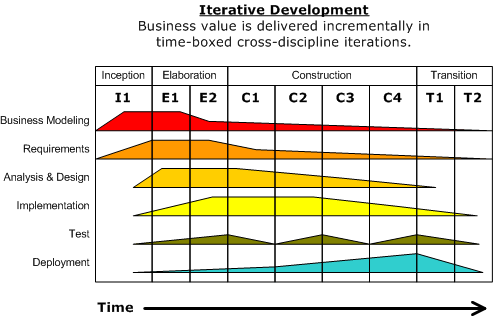
\includegraphics[scale=0.7]{./Figures/RUP.png}
	\caption[Rational Unified Process]
	{Iterative development cycle of Rational Unified Process.}
	\label{fig:RUP}
\end{figure}

Now we have acknowledged some development processes that are commonly used in
the industry for creating software applications. Model Driven Engineering is a
software development methodology that focus on creating and exploiting
models. And by using these models, MDE aims at improving productivity and
quality in a software developments\cite{France2007}. This is achieved by not only to use
models as documentation, but instead use models as the major artifact in a software
development cycle. The idea is to use models at different levels of abstraction
and apply model transformations to automate the implementation of these
models. This will raise the level of abstraction in program and problem
specification. We can divide these models into two main model classes, namely
development models and runtime models. Development models are used as an
abstraction above code level. These models can represent software
requirements, work flow, architecture and software implementation. These
development models are most commonly used in software development processes as a
supplement in developing an application. Runtime models represents executable
systems of a software application. Example of such executable systems are
database operations or computations of data. There has been an increase in MDE
researchers that explore how runtime models can be used to support dynamic
adaptation of systems for a software application\cite{France2007}. The idea for
MDE is to be able to specify these development models as runtime models and
evolve software applications with the use of runtime models and development
models as major artifacts of a development process. 
 
A typical Model Driven Software Engineering (MDSE) scenario is to obtain an
executable software application through model transformations that produce a
more and more detailed version of the application until an executable version is
created. We reach this level of automation by applying model transformations to
models at higher levels of abstraction and producing models that contains a more
detailed description of the software. This highlights one main advantage of a
model driven approach, and that is to bridge the communication gap between
requirements/analysis and implementation\cite{Brown2008}. For a traditional
development process today there is a gap in communication between software
developers and customers\cite{France2007}. Because a customer is usually not an
expert in designing and implementing a software application. A customer can
provide a set of requirements for a software application and take part in
analysing these requirements to make sure that the development team shares the
customers thought of the program. The requirements and analysis can be
specified down to every detail, however a software application might experience
different design choices that leads to a different implementation of the
application compared to what the costumer initially specified. If the visions
of MDE is adopted to a software development process then this could help to
narrow the gap in communication between developers and stakeholders. Because
now we can apply model transformation that changes input models to target
models that represents both the design and the executable implementation of a
software application. We will describe model transformations and their purpose
in model driven engineering in more depths in chapter~\ref{Chapter3}. Models
that are provided at different level of abstractions is less complex than
several thousand lines of implementation code. This represents another benefit
of adopting MDSE into the development process. Because models captures and
organize the understanding of a system that results in a more clear discussions
among team members and new team members. One approach that introduces modeling
at different level of abstraction for including MDSE in a software development
process is the Model Driven Architecture.

\subsection{Model Driven Architecture}
\label{MDA}

Model Driven Architecture (MDA) is an industry architecture developed by the
Object Management Group (OMG) that address the possibility to provide automation
according to models in an application development cycle.
MDA is a proposal for applying the practices of MDE to a system development. This
architecture is a good example to use when we are discussing concepts of MDE,
because of its similarity to a traditional software development process. Since
it has support for standard phases in a software development process such as
analysis, design and implementation. Many organizations have adopted MDA as a
reference framework to include the concepts of MDE. One reason for this is the
importance of OMG for the software industry. MDA is build around many
concepts that OMG has released, such as the OMG specifications the Unified
Modeling Language (UML) and the Meta Object Facility(MOF).

\begin{figure}[H]
	\centering
	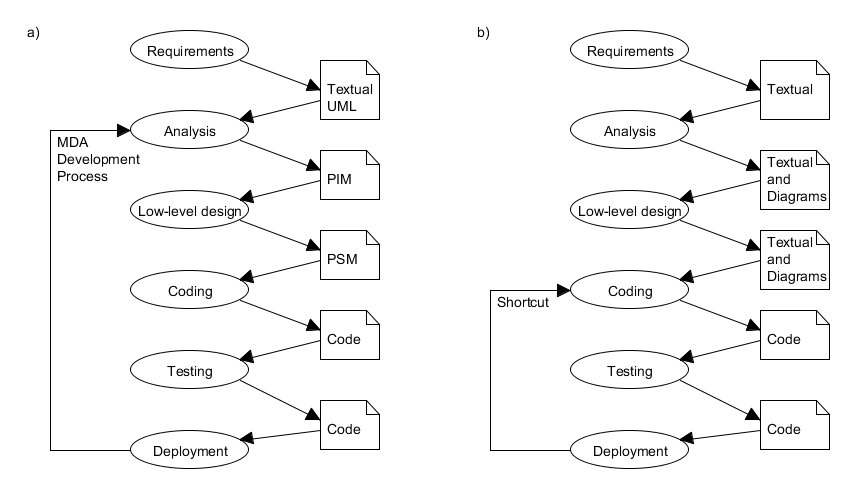
\includegraphics[scale=0.5]{./Figures/MDA.png}
	\caption[Software Development with MDA]
	{a) Model-Driven-Architecture and b) Traditional development process}
	\label{fig:MDA}
\end{figure}

Figure~\ref{fig:MDA} gives a representation of the development process that the
Model Driven Architecture provides and a traditional development process on the
right side.
Both of the approaches have similar starting phases, where a customer presents a
list of requirements for a software application. The process to create
implementation code from the requirements is where a MDE approach to software
development is different. Because for MDA the idea is to use models instead of
text and diagrams for the analysis and design phase. For a traditional
development process these phases usually consist of creating diagrams that
describes different system of the application. In MDA these diagrams or models
are the main artifact for the corresponding phases, instead of just a reference for
developers to use when implementing an application. The architecture then
propose that implementation code is generated based on these models. A
traditional software development process would have iterations for the
implementation and testing to make sure that the application meets the demands
of the customer. This process is continued for every iteration, where
developers continually use the text and diagrams that was created earlier in
the process. The idea for an MDA development process is to provide automation
between models created at each development phase. Instead of going back to the
code and do corrections and modifications on the application a model driven
software development process goes back to analysing the problem and modify the
models accordingly. With the power of automatically changing models from one
phase to another and generate implementation code from the models at the last
level of abstraction.

Figure~\ref{fig:MDA_PLATFORM} provides a representation of the models at the
different layer of abstractions that is part of the Model Driven Architecture. 

\textbf{Computation-Independent Model (CIM)} is the most abstract level of
modeling and is often referred to as a business model or domain model. The
model does not contain any computational implications to how the software
application should behave, but express exactly what the final application
should do. This model remains independent to how a system will be or currently
is implemented and represents the requirements and purpose of the system. A
Computation-Independent Model is often described by using a natural language to
define the requirements for a software application. 

\begin{figure}[H]
	\centering
	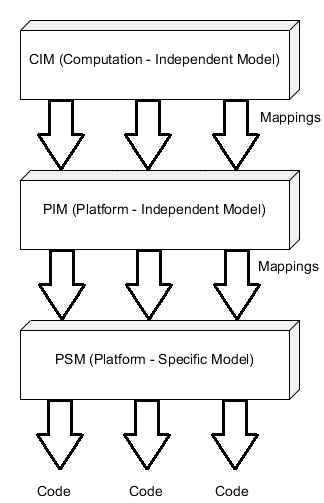
\includegraphics[scale=0.7]{./Figures/MDA_Platforms.png}
	\caption[The three levels of modeling abstraction for MDA]
	{The three levels of modeling abstraction that MDA provides.}
	\label{fig:MDA_PLATFORM}
\end{figure}

\textbf{Platform-Independent Model (PIM)} is the level of abstraction that
describes the behavior and structure of a software application. This model is
platform independent, which means that the technological platform used to
implement the software application is not defined. A Platform-Independent Model
will only address tasks that a software application can perform. These tasks
are part of the context of the business model at the top level of abstraction.

\textbf{Platform-Specific Model (PSM)} is the level of abstraction that contains
all required information for the behavior and structure of a software
application that is linked to a specific technological platform. These specific
platform technologies can be a specific programming language like a general
purpose programming language, a specific operation system or a specific database
technology. The Platform-Specific Model contains all the information that is
required for an actual implementation of the application. 

In MDA, the core activity is the starting phase, which is to analyse the
problem at hand. Requirements are firstly defined and modeled as a CIM or a PIM.
The CIM and PIM provides the solution for the requirements at a very high level
of abstraction. The computation independent level of abstraction we provide
the requirements of a solution without thinking about the actual implementation
of an application. A CIM specifies the workflow of an application and how end
users utilizes the application. For example the model could define the
requirements for a web application that provides a collection of goods that the end users can purchase.
These requirements could specify how an employee performs tasks when a new order
arrives. For the implementation of an application not all of these requirements
are necessary. The purpose of MDA is that models created at
CIM level provides the highest level of abstraction and therefore should be
readable by everyone. In figure~\ref{fig:MDA_PLATFORM} MDA suggest
that new models are created accordingly based on a set of mappings. Models that
is provided at the platform independent abstraction is not concerned with
technologies that should be used for the actual implementation. PSM is more
concerned with describing what tasks an application should perform. But tasks
that an employee should perform, like for example making a shipment ready for
transportation is not defined in a PIM. A platform specific model specifies what
implementation platform and a set of precise descriptions of the technical
details of the corresponding implementation platform. Mapping a model to another
model is essential for applying MDA to a development process. A mapping defines
correspondences between elements of two different models and can be defined
between all different models.

\section{Modeling Languages}

A Modeling language is defined through three core concepts. Regardless if its
either a Domain Specific Modeling Language (DSML) or a General Purpose Modeling
Language (GPML). Figure~\ref{fig:modeling_language} represents the three main
concepts for a modeling language.

\begin{figure}[H]
	\centering
	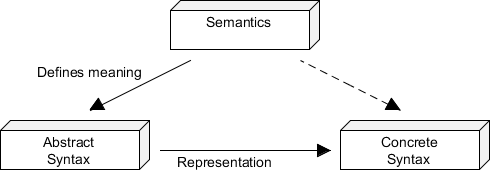
\includegraphics[scale=0.7]{./Figures/modeling_language.png}
	\caption[Main ingredients of a modeling lanugage.]
	{The three main ingredients of a modeling language.}
	\label{fig:modeling_language}
\end{figure}

A modeling language has an abstract and a concrete syntax. The abstract syntax
describes the structure of the modeling language and how modeling elements can
be combined together. The concrete syntax on the other hand describes a specific
representation of the abstract syntax, and can either be a graphical or
textual representation. The semantics of a modeling language describes the
meaning of these modeling elements and the different ways to combine them for
the abstract syntax and indirectly the concrete syntax. We mentioned DSML and
GPML, where these two modeling languages represents one of the main
classification of modeling languages. A modeling language can either be
classified as a domain specific or a general purpose language. DSMLs are
modeling languages that are designed for a specific domain or a concept. While
GPMLs are modeling languages that is applicable for several different domains.
A general purpose language lacks features that are special for a particular
domain. This is one of the strengths for DSLs that is created especially for a
certain domain, and therefore provide more details to a specific domain compared
to a general purpose language. The Unified Modeling Language\cite{UML_SPEC}
(UML) is an example of a general-purpose modeling language that
was accepted in 2000 by the International Organization for Standardization
(ISO) as an industry standard for modeling software systems. UML was initially
developed by Grady Booch, Ivar Jacobsen and James Rumbaugh at Rational Software
in the 1990s. It was later adopted by the Object Management Group in 1997 and
has since this day been continuously developed by the organisation. UML is
often called a general purpose language because it is often referred to as a
suite of languages, since it provides developers and designers with the possibility to
specify applications through several different modeling languages, or diagram
types that UML often is associated with. However, in the book, ``Model-Driven
Software Engineering in Practice'' published by Marco
Brambilla, Jordi Cabot and Manuel Wimmer in 2012, they state the following.
\textit{If we think to the general modeling problem, we can see UML as
a DSL tailored to the specification of (mainly object-oriented) software
systems\cite{Brambilla:MDSE}.} This means that to decide whether UML is a DSL or
a GPL is not a binary choice. But we mostly see UML as a general purpose
modeling language, since it offers a wide variety of modeling languages that
designers and developers can use to specify system abstractions. Whether a
modeling language is classified as a general purpose or a domain specific
modeling language it requires that it is described by an abstract syntax. Both
the abstract syntax and the concrete syntax of a modeling language is
represented as models. Therefore the specification of the abstract syntax is
often referred to as a meta-model. 

\subsection{Meta-modeling}

Models are a major artifact in the concept of model driven engineering (MDE). It
is essential to look at every model as instances of some more abstract model.
And therefore we can define a meta-model as yet another abstraction that
highlights the properties of an instance model. Meta-modeling represents a vital
part of MDE and constitutes the definition of a modeling language. A meta-model
defines the abstract syntax and provides a description of a modeling language.
Another popular definition for describing a meta-modeling is that it is a
``model of models". This definition is both unhelpful and incorrect according
to Steve Cook and Stuart Kent in their paper\cite{Cook2008} published in 2008.
They think that a better definition for a meta-model is that ``it is a model of
the concepts expressed by a modeling language.'' The exact definition of a
meta-model is highly debated amongst MDE researchers\cite{Rutle_thesis}.

\begin{figure}[H]
	\centering
	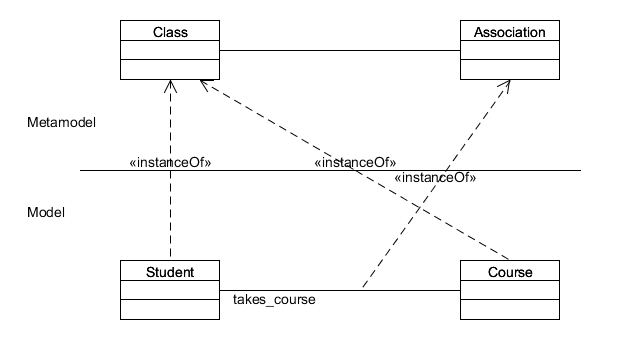
\includegraphics[scale=0.6]{./Figures/SimpleMetamodel.png}
	\caption[Example of a model and meta-model]
	{A simple example of a model and its meta-model.}
	\label{fig:SimpleMeta-model}
\end{figure}

Figure~\ref{fig:SimpleMeta-model} shows a simple example of an instance model
and its corresponding meta-model. This model has two classes, Student and Course, and
a bidirectional association, take course and has students, that relate
these two classes. The model is specified by a meta-model that consists of two
meta-classes Class and Association and an association between them. Both Student
and Course are an instance of the meta-class Class, while the association
between Student and Course are instance of the meta-class Association. The
modeling language that describes this model corresponds to the Unified Modelling
Language.

\subsubsection*{Meta-Object Facility}

The Meta-Object Facility\cite{MOF} (MOF) is an Object Management Group standard
for defining meta-models in MDE. The Object Management Group was in need of a
architecture to define the UML. Through this process of finding a common
platform for UML, OMG designed a four layered architecture that provides a
semi-formal approach to creating meta-models. MOF later became a language for
defining abstract syntax for modeling languages. 

\begin{figure}[H]
	\centering
	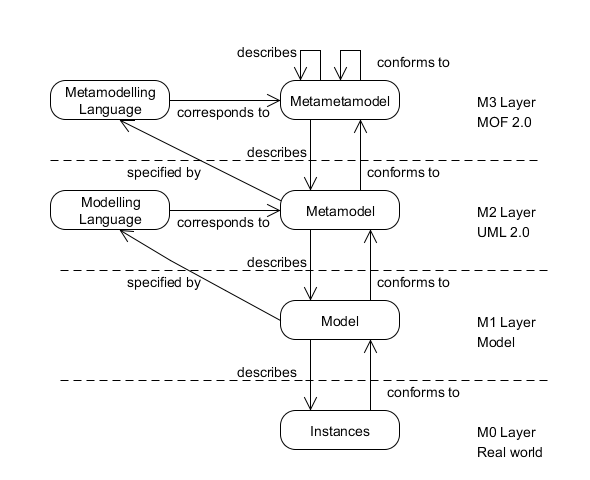
\includegraphics[scale=0.6]{./Figures/MOFLayers.png}
	\caption[Meta Object Facility]
	{Example of Meta Object Facility and its four layers.}
	\label{fig:MOFLayers}
\end{figure}

Figure~\ref{fig:MOFLayers} gives a impression of the four layers that are
available in the Meta-Object Facility. At the top level, M\textsubscript{3},
there is a meta-meta-model called MOF. This meta-meta-model is meant to both
describe it self and conform to itself. MOF is then used to describe meta-models
at the M\textsubscript{2} level. The UML meta-model is an example of such a
meta-model. The idea is that these meta-models are specified by some
meta-modeling language that corresponds to MOF. Models at the M\textsubscript{2}
layer represents the abstract syntax for models created in the M\textsubscript{1} layer. This
layer represents models that are created by some modeling language, like
for example UML. Finally at the M\textsubscript{0} we have an instance model of
a real world object. If we refer to our simple example concerning a model and
its corresponding meta-model in figure~\ref{fig:SimpleMeta-model}. From this
example we can create a real world object of that model, ``Petter Barvik'' takes
a course in Model Transformations. MOF provides meta-modeling architecture where
every modeling element on every layer corresponds to some modeling element
one layer higher. One could say that MOF itself a Domain Specific Language (DSL)
to create meta-models. 
 
\subsection{Constraints}

Constraints impose conditions that modeling elements must satisfy and helps
to define the semantics of a domain specific language. A constraints can be
compared to a Boolean condition. Boolean conditions are either true or false,
while constraints are either satisfied or not satisfied. Including constraints
to modeling elements in the abstract syntax specifies how modeling elements
are presented in an instance model. Modeling elements that are included in the
abstract syntax can have constraints defined on objects, classes, attributes, links,
associations, etc. A constraint is a restriction for how these elements should
behave. Constraints on elements such as those above can be expressed with a
natural language or by a formal language, such as the Object Constraint
Language\cite{OCL} (OCL). The Object Constraint Language (OCL) is a declarative
programming language for describing constraints that applies to UML models.
Before UML became an adopted standard of the Object Management Group (OMG), OCL
was an extension language to UML. Now OCL can be used with any Meta-Object
Facility (MOF) meta-model, including UML. A software developer can in
combination with UML and OCL define the semantics for a modeling
language\cite{Warmer:2003:OCL:861416}.

The difference between object and classes needs to be specified. A class
is often a meta element for an object. This means that a class could be part of
a model that describes an object element, and therefore an object element is
typed by the class element\cite{OO_UML}. Figure~\ref{fig:SimpleMeta-model}
describes the two object elements Student and Course that are an instance of the
meta-element Class.

\begin{figure}[H]
	\centering
	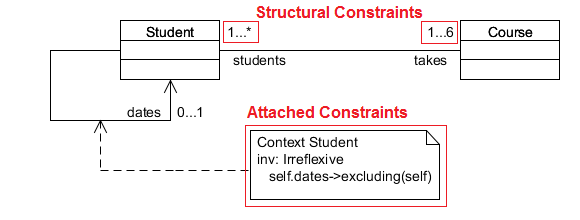
\includegraphics[scale=0.7]{./Figures/Constraints.png}
	\caption[Simple model with constraints]
	{Example of a simple model with attached and structural constraints.}
	\label{fig:Constraints}
\end{figure}

These restrictions on modeling elements can either be a structural constraint or
an attached constraint. These structural constraints are defined in the structure
of the models. In figure~\ref{fig:Constraints} we have extended the model we
introduced in figure~\ref{fig:SimpleMeta-model} with some  modeling elements. We
have created an association that specifies that a student can date other
students. In this model we can see that the model has three multiplicity
constraints that are part of the models structure. A multiplicity constraint for
an association restricts the number of objects that are related to a given
object. From the association constraint on this model we can see that a student
requires to take at least one course and up to a maximum of six courses. The
models restricts a student to not participate in any courses. The second
structural constraint requires a course to have at least one student for
this course to be part of a semester, and the course can have an arbitrary
maximum number of students participating the course. The association dates,
between two students for this model has an attached constraint that is
specified in the declarative language OCL. The general form of an attached
constraint has a context, in this case a Student, that specifies what object the
constraint includes. The attached constraint has a name \textit{``Irreflexive''}
followed by a Boolean OCL expression that explicitly refers to itself. This constraint
specifies that a student is unable to date her or him self. Constraints has a
vital part in model driven engineering to measure the quality and precision of a
model. A model without constraints does not work in practice. In
\textit{The Object Constraint Language: Getting Your Models Ready for
MDA}\cite{Warmer:2003:OCL:861416}, Jos Warmer and Anneke Kleppe states that a
model without constraints would be severely underspecified. Constraints
expressions written in OCL are unambiguous and results in a more precise and
detailed model. If we where to remove both the structural and attached
constraints from figure~\ref{fig:Constraints} then the model is less
informative. There is no understanding on how the objects are related to
one another. 

\section{Language Workbenches}

Language workbenches are tools that lets user specify
their own Domain Specific Language (DSL) and include editing tools for the newly
created language. A workbench should consist of Integrated Development
Environment (IDE) that lets users create their own DSMLs.
Figure~\ref{fig:langauge_workbench} is provided in the paper, \textit{``DPF
Workbench: a multi-level language workbench for MDE"}, that was published by
Yngve Lamo, Xiaoliang Wang, Florian Mantz, {\O}yvind Bech, Anders Sandven and
Adrian Rutle in 2013. The figure presents the intended use of language
workbenches and consist of two phases. The first handles the definition of a
new DSML and the creation of tool support such as code generation, editors,
model transformations, etc. A language workbench is created by a domain expert
in collaboration with an experienced developer. The latter describes the actual
usage of this newly created workbench, where developers can utilize the DSML
environment to create models, generate implementation code, etc. Language
workbenches are a very young field in computer science, and there are many
existing solutions that is open for the public to use. These concepts have the
potential to change the face of programming as we know
it\cite{fowler2010domain}, but the concepts of workbenches are still fresh to
computer science.

\begin{figure}[H]
	\centering
	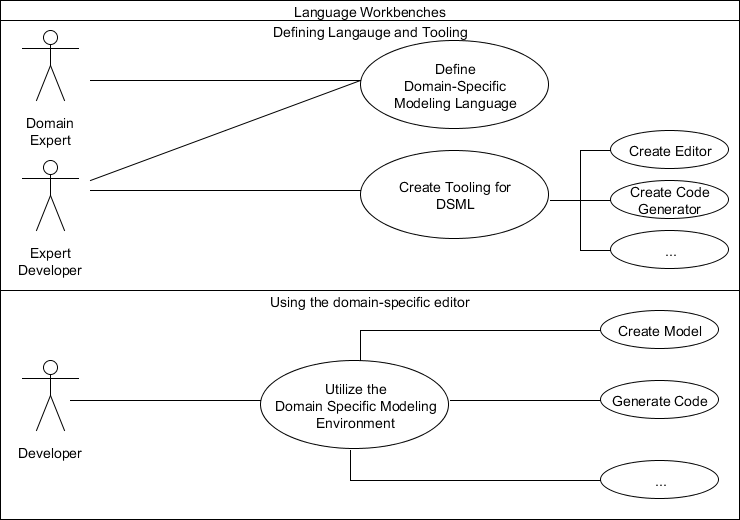
\includegraphics[scale=0.6]{./Figures/langauge_workbehcn.png}
	\caption[Intended use of language workbenches]
	{Intended use of language workbenches.}
	\label{fig:langauge_workbench}
\end{figure}

The concepts behind a language workbench is that the tool does not just provide
the users with an IDE to create DSLs, but also generates a new IDE where this
newly created DSL can be edited. In addition to an IDE that provides creation
and editing of a newly created language a workbench should define support for
code generation, model transformation, model versioning, etc\cite{Lamo2013}.
Figure~\ref{fig:workbench} describes components for a language workbench. Martin
Fowler describes three main parts to defining a new language workbench in his
paper\cite{fowler2005language}:

\begin{figure}[H]
	\centering
	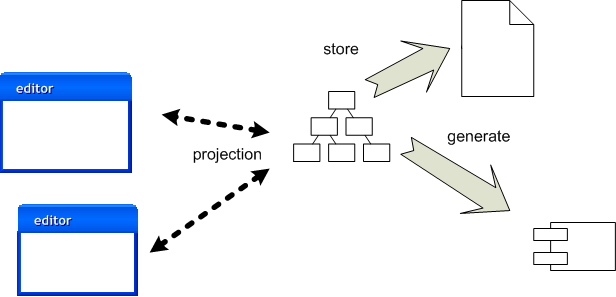
\includegraphics[scale=0.6]{./Figures/workbench.png}
	\caption[Components of language workbenches]
	{Components of language workbenches.}
	\label{fig:workbench}
\end{figure}

\begin{itemize}
  \item The abstract representation for the language.
  \item One or more editing environments for the language.
  \item Defining the semantics behavior of the language. 
\end{itemize}

\subsection{EMF}

Eclipse Modeling Framework is originally based on Meta Object Facility (MOF)
provided by the Object Management Group (OMG). In 2003 EMF designers contributed
to designing the MOF 2.0 version of the standard that was later named Essential
MOF (EMOF). EMF provides the meta-model Ecore that is aligned to EMOF and is a
general purpose modeling language to create modeling languages. Ecore is
essentially a simplified version of class modeling in UML.

\begin{figure}[H]
	\centering
	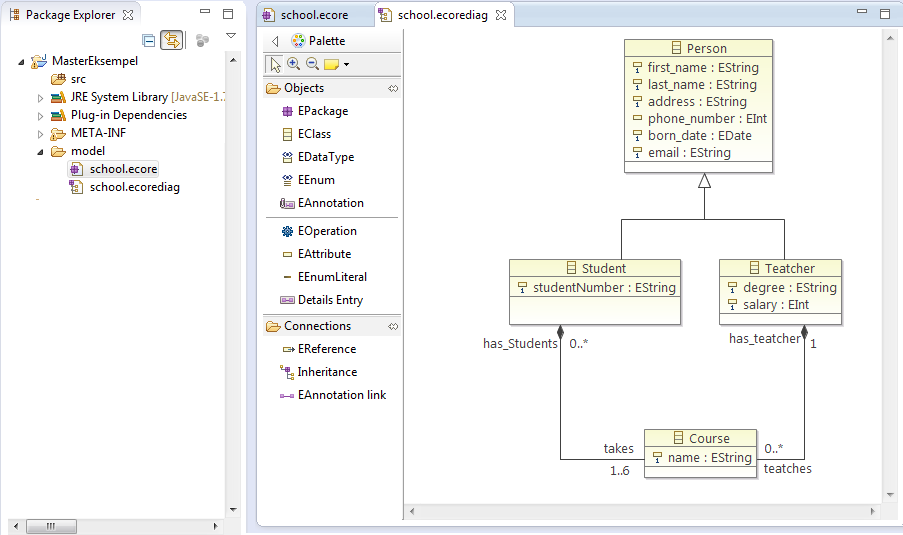
\includegraphics[scale=0.6]{./Figures/EMF_Diagram_Picture.png}
	\caption[Ecore model represented by Ecore Tools]
	{A graphical representation of an Ecore model.}
	\label{fig:EMF_Diagram}
\end{figure}

Figure~\ref{fig:EMF_Diagram} represents an Ecore model that is created from a
graphical editor. This Ecore model conforms to the Ecore meta-model and is the
core language for EMF. The framework provides a two layered approach to
meta-modeling where the user can create a DSL based on the Ecore meta-model.
Based on the DSL the framework provides code generation facilities. Amongst
generating java implementation for the model the framework also provides code
generation for an editor that is based on the DSL. This editor can be used to
create instances of the defined DSL. 

% \subsection{Visual Modeling and Transformation System}

% \begin{figure}[H]
% 	\centering
% 	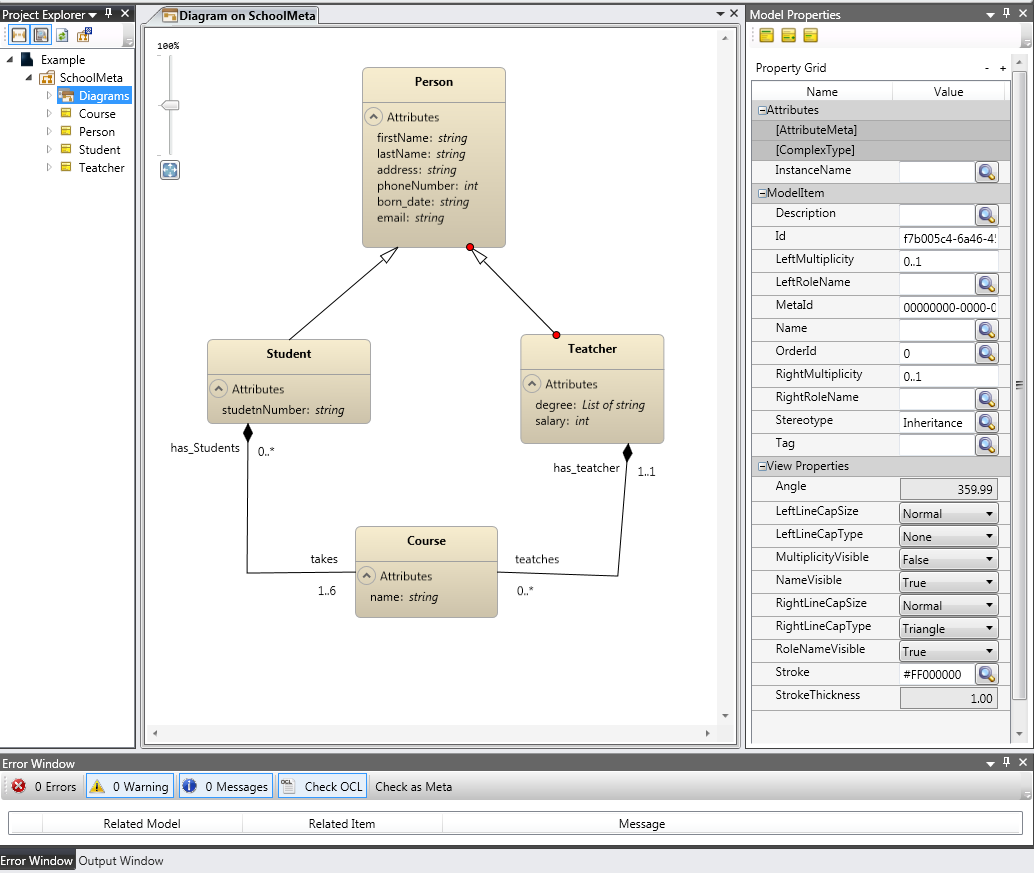
\includegraphics[scale=0.5]{./Figures/VMTS}
% 	\caption[Creating domain specific modeling language in VMTS]
% % 	{Specifying a domain specific modeling language in VMTS.}
% 	\label{fig:VMTS}
% \end{figure}

\section{Diagram Predicate Framework}
\label{sec:DPF}

Diagram Predicate Framework\cite{Rutle_thesis,Rossini_thesis,Lamo2013} (DPF) is
an ongoing research project that was first initiated by Bergen University
Collage and the University of Bergen in Norway 2006. With features likes
meta-modeling, model transformation and model management, DPF aims at
formalising concepts of model-driven engineering. DPF is based on category
theory and graph transformations and is an extension of the Generalised
Sketches\cite{Diskin2003} formalism that was initially developed by Zinovy
Diskin.

In October 2002 Dominique Duval published a paper where he specified that a
specification can be considered as a directed graph with additional structure
in the same way that a theory can be considered as a category with additional
structures\cite{Duval2003}. Generalised Sketches by Zinovy Diskin utilize the
concept of sketches. A sketch, first introduced by Ehresman in 1966, is a
directed graph that provides additional properties, such as colimit, limit and
constraints. DPF utilize these concepts through an diagrammatic approach to
meta-modeling and to facilitate the concepts of MDE. The framework provides the
possibility to define an unlimited layers of meta-modeling. In DPF models are
represented as specifications.

\begin{itemize}
  
\item A \emph{specification $\spec{S}$} = (S,
C\textsuperscript{$\spec{S}$}:$\Sigma$) consist of an underlying graph S and a
set of atomic constraints C\textsuperscript{$\spec{S}$}. 

\item Atomic constraints are specified by predicates from a predefined signature
$\Sigma$.

\item A signature $\Sigma$ = ($\Pi$ \hspace{1 mm}, \hspace{1 mm}$\alpha$)
consist of a collection of predicates. 
  
\end{itemize}

A \emph{specification $\spec{S}$} has an underlying graph S that contains
modeling elements that defines the model structure of the specification. These
modeling elements are always represented as a node or an arrow. However these
nodes and arrows could be specified through several layers of
meta-models or specifications. The \emph{specification $\spec{S}$} also consist
of a set of constraints, these constraints will restrict the model structure of
a new instance model of this specification. Figure~\ref{fig:DPF_Spec} presents a
specification $\spec{S}$\textsubscript{2}, that is defined by an underlying
specification $\spec{S}$\textsubscript{3} and describes a modeling language for
some $\spec{S}$\textsubscript{1} specification. This specification includes two
nodes Condition and Activity, two arrows ChoiceOut and Message and  two sets of
atomic constraints. The first constraint defines that a Condition element has
to be connected to exactly one Activity element for this structure. The second
constraints specifies for this graph structure that an Activity element cannot
be associated with it self. These constraints examples are specified as a
collection of predicates from a predefined signature $\Sigma$. The table in
figure~\ref{fig:DPF_Spec} represent some of the predicates from this
collection. A predicate is represented by an unique symbol $\Pi$, a shape graph
$\alpha$, a proposed visualisation and a semantic interpretation

\begin{figure}[H]
	\centering
	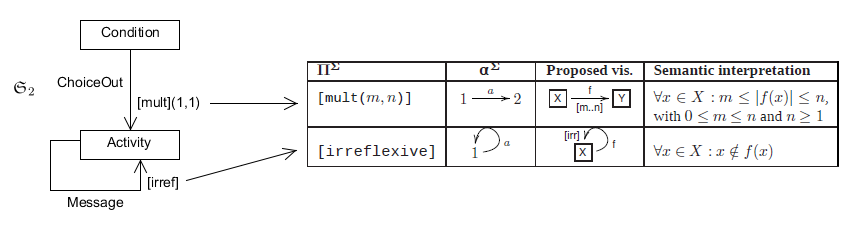
\includegraphics[scale=0.7]{./Figures/DPF_spec_constraints.png}
	\caption[A specification and some predefined diagrammatic predicate attached]
	{A specification $\spec{S}$\textsubscript{2} with some attached predicates.}
	\label{fig:DPF_Spec}
\end{figure}

An instance specification $\spec{S}$\textsubscript{n} that is initialised from
a specification $\spec{S}$\textsubscript{n+1} defines a graph homomorphism
between two underlying graphs. There is a graph homomorphism,
S\textsubscript{n}$\longrightarrow$S\textsubscript{n+1}, between the underlying
graph S\textsubscript{n} of a specification $\spec{S}$\textsubscript{n} and the
underlying graph S\textsubscript{n+1} of
a specification $\spec{S}$\textsubscript{n+1}\cite{Lamo2013}. The graph
homomorphism S\textsubscript{n}$\longrightarrow$S\textsubscript{n+1} must
satisfy a set of atomic constraints, C\textsuperscript{$\spec{S}$} from a
specification $\spec{S}$\textsubscript{n+1}.
Figure~\ref{fig:modeling_formlalism} from Adrian Rutle's dissertation,
 \textit{Diagram Predicate Framework A Formal Approach to
MDE}\cite{Rutle_thesis} that was published in 2010 represents an example of a
specification that is defined by a modeling formalism. 

\begin{figure}[H]
	\centering
	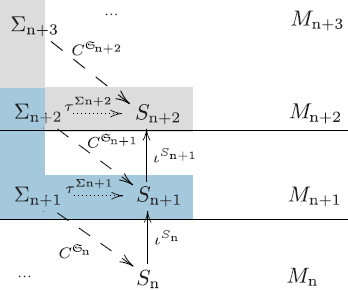
\includegraphics[scale=0.7]{./Figures/modeling_formlalism_adrian.png}
	\caption[Modeling formalism in DPF]
	{Meta-modeling represented as modeling formalism's in DPF.}
	\label{fig:modeling_formlalism}
\end{figure}

Because in DPF a modeling language at a specific abstraction layer is
represented as a modeling formalism.
A modeling formalism in DPF is defined by a set of atomic constraints from a
modeling formalism one abstraction layer higher and a specification that has an
underlying graph and a set of atomic constraints. For example figure~\ref{fig:modeling_formlalism} represents three levels of
abstractions for defining a DSML. The specification $\spec{S}$\textsubscript{n}
that is defined at M\textsubscript{n} layer conforms to the modeling
formalism one layer higher. The modeling formalism consist of a specification
$\spec{S}$\textsubscript{n+1} that has an underlying graph S\textsubscript{n+1}
and a set of predicates Z\textsubscript{n+2}. Together with specification
$\spec{S}$\textsubscript{n+1} a set of predicates Z\textsubscript{n+1} can be
defined to specify a new modeling formalism for lower layer of abstractions. 
modeling formalism\cite{Rutle_thesis}. This defined modeling language, or
modeling formalism provides the abstract syntax that can be used to create a
specification or modeling formalism one abstraction layer lower. What is special
with DPF is that a modeling formalism represents both the abstract syntax for
a specification one abstraction layer lower and the concrete syntax for a
specification one abstraction layer higher. The set of atomic constraints
Z\textsubscript{n+1} provides the semantics and the
specification $\spec{S}$\textsubscript{n+1} provides the abstract syntax for
defining modeling elements in a new specification $\spec{S}$\textsubscript{n}.
Figure~\ref{fig:MOF_vs_DPF} explains the difference between OMG's MOF and DPF's
multi-layered meta-modeling hierarchy.

\begin{figure}[H]
	\centering
	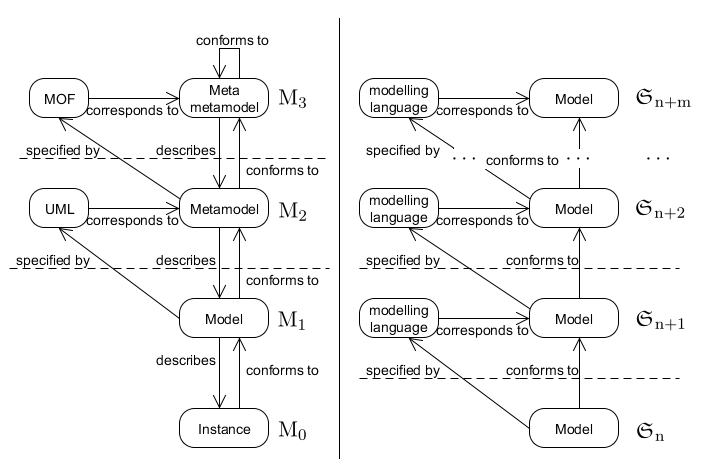
\includegraphics[scale=0.7]{./Figures/MOF_vs_DPF}
	\caption[OMG's layers of meta-modeling and multilayer modeling]
	{OMG's layers of meta-modeling and an arbitrary layer of meta-modeling.}
	\label{fig:MOF_vs_DPF}
\end{figure}

These two sides highlights the differences between DPF and modeling environments
that expand MOF to create modeling languages. While MOF based modeling
environments provides two abstraction layers, DPF on the other hand provides an
unlimited abstraction layers users can interact with. The reason that MOF based
modeling environments provides two layers to interact with is because the
layers M\textsubscript{2} and M\textsubscript{3} are usually part of the
environments internal infrastructure. For example in EMF users can create
models that conforms to the Ecore meta-model. The only meta-model that users of
DPF are unable to interact with is located at the highest abstraction layer. A
specification $\spec{S}$\textsubscript{n+1} is specified by a modeling language
that corresponds to a specification $\spec{S}$\textsubscript{n+2}. But the same
specification $\spec{S}$\textsubscript{n+1} also represents the abstract syntax
for a specification $\spec{S}$\textsubscript{n}. These DPF models automatically
generates a new graphical editor environment provided by the DPF Workbench.

\section{DPF Workbench}

The DPF Workbench provides a modeling environment for DPF and consist of three
main components. These are the ``DPF Model Editor'', the ``DPF Signature Editor''
and the ``DPF Code Generator''. The first two editors provides the modeling
functionality for the DPF Workbench. ``DPF Model Editor'' is used to create and
modify DPF specifications. The ``DPF Signature Editor'' is used as a supplement
to the ``DPF Model Editor''. It provides an editor to construct user defined
predicate signatures. These signatures can then be used to define the semantics
of a DPF specification in the ``DPF Model Editor'' if the predefined predicates
that DPF provides does not suffice. Figure~\ref{fig:DPF_Editor} that is
provided in the article\cite{Lamo2013}, explains how the ``DPF Signature Editor'',
the ``DPF Model Editor'' and a DPF Model is related to each other in the DPF
Workbench over different abstraction layers. The ``DPF Code Generator'' provides
the users with a code generation environment for DPF specifications.  

\begin{figure}[H]
	\centering
	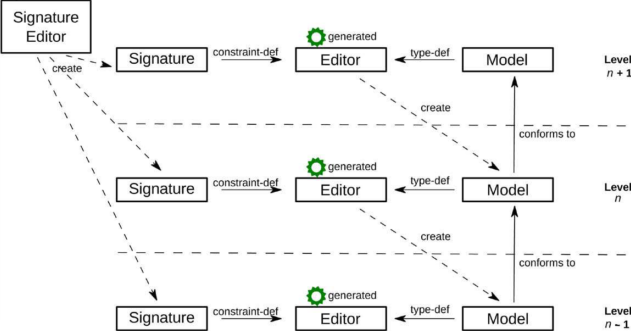
\includegraphics[scale=0.7]{./Figures/DPF_Workbench}
	\caption[DPF Editor in multi-layer meta-modeling hierarchy]
	{Generated DPF Editors in a multi-layer meta-modeling hierarchy.}
	\label{fig:DPF_Editor}
\end{figure}

\subsection*{DPF Model Editor}
The DPF Model Editor is an extension of the Diagram Predicate Framework that
provides an intuitive approach to creating modeling languages and have been created
using several different technologies. In 2011 $\O$yvind Bech published his
master thesis\cite{Bech_thesis} where he designed the implementation of
the DPF Model Editor that is based on the Eclipse Modeling Framework technology.
This first version of the DPF Model Editor has seen several iterations and provides
support for creating domain specific modeling languages.
Figure~\ref{fig:DPF_Editor} explains that a new instance of the DPF Model
Editor is generated for each new model that is created. This means that every
DPF specification has a corresponding editor that provides graphical editing
properties to change the models. For each generated editor we can create a new
DSL one abstraction layer lower that generates a new editor that correspond to
this DSL.

% \subsection*{DPF Signature Editor}
% 
% \subsection*{DPF Code Generator}

%  
% \begin{table}[ht]
% \renewcommand*\arraystretch{1.5}
% \centering
% \begin{tabular}{| c | c | c | c | c | c |}
% \hline
% Tool & Layers & Dia.   & Const.   & Platform & GUI\\
% 	 & 		  & Const. & Language &          & \\
% \hline
% EMF/GMF & 2 & & OCL, EVL, & Java VM & $\surd$ \\
% 		%&  	& & Java      &         & \\
% \hline
% VMTS    & $\infty$ & & OCL & Windows & $\surd$ \\
% \hline
% AToM\textsuperscript{3} & 2 & & OCL, Python & Python, Tk/tcl & $\surd$ \\
% \hline
% GME  & 2 & & OCL & Windows & $\surd$ \\
% \hline
% metaDepth & $\infty$ & & EVL & Java VM & \\
% \hline
% DPF & $\infty$ & $\surd$ & Predefined & Java VM & $\surd$ \\
% 	& 		   &         & validator  &         & \\
% \hline
% 
% \end{tabular}
% \caption{Comparing model transformation tools.}
% \end{table} 
 
% Chapter Template

\chapter{Model Transformation} % Main chapter title

\label{Chapter3} % Change X to a consecutive number; for referencing this
% chapter elsewhere, use \ref{ChapterX}

\lhead{Chapter 3. \emph{Model Transformation}} % Change X to a consecutive 
% number; this is for the header on each page - perhaps a shortened title

%----------------------------------------------------------------------------------------
%	SECTION 1
%----------------------------------------------------------------------------------------

Transformation are a fundamental aspect in computer science and software
engineering. Whenever a computer starts up, transformation of computer systems
and computer programs happens frequently. Take a compiler for instance, it plays
a vital part of a computers internal infrastructure. A compiler is a computer
program that translates source code written in a high-level programming
language into a lower level language, such as an assembly language or machine
code. This means that a computer program written in a general-purpose
programming language, such as Java or C++ would be useless without a compiler,
since the computer's central processing unit (CPU) depends on machine code to be
able to execute a set of instructions. But also computation of primitive data
values and performing operations on data structures such as lists and arrays can
also be viewed as data transformations. When a programming language provides a way
to type these data values or data structures, then a compiler or interpreter can
apply operations to the data accordingly to the type. But when we mention
data representing software artifacts such as a data schema, programs or models,
then transformation approaches 

%-----------------------------------
%	SUBSECTION 1
%-----------------------------------
\section{Basic concepts of model transformation}

The very basic concept of a model transformation on the highest level of
abstraction is to translate one model to another model. This model translation
can either be achieved through an endogenous or an exogenous model
transformation. For an endogenous model transformation we take a source model
expressed in a modeling language and produce a target model expressed in the
same language. While an exogenous model transformation start with a source
model expressed in one modeling language and translate this into a target model
expressed in another modeling language. It is essential that these models
remain consistent, and therefore both the source and target model have to
conform to their corresponding meta-model.

\begin{figure}[H]
  \centering
    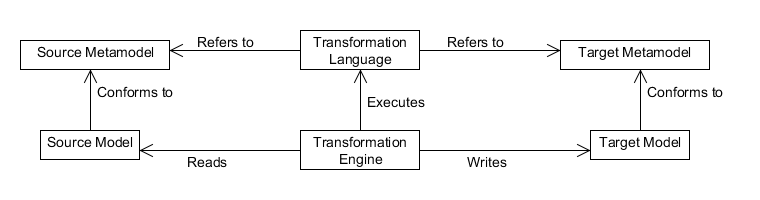
\includegraphics[scale=0.5]{./Figures/BasicTransformation.png}
    \rule{35em}{0.5pt}
  \caption[Basic Model Transformation]
  {The basic concepts behind a model transformation.}
  \label{fig:BasicTransformation}
\end{figure}

Figure~\ref{fig:BasicTransformation} is a representation of the basic concepts
for a model transformation. The two concepts, transformation language and
transformation engine are provided by some model transformation environment.
The main idea behind changing two models are to read a source model and write a
target model. The transformation engine executes a transformation language that
specifies a set of guidelines that express how the target model is constructed.
These guidelines is created from meta-data that are defined in the source and
target meta-model to create an executable environment for the transformation
engine. Where the transformation language use both the source and target
meta-model as a reference point when specifying these guidelines for the source
and target model. The transformation language specifies how a translation
between two models should be applied through the use of these meta-models. Both
meta-models provides some abstract syntax that a transformation language can
utilize to specify a model transformation environment. One aspect behind the
abstract syntax that should be taken into consideration is that the concrete
syntax of the abstract syntax can be either textual or graphical. Traditionally
when we use the concept model, we think of a miniatures, with nodes and
vertexes that are connected with arrows and edges. These miniatures represent a
graphical representation of a model. However a model can also have a textual
representation. Therefore we often say that a model transformation can produce
two different kind of target models. At the highest level of abstraction these
two different target models can either be produced by a Model to Text (M2T)
transformation or a Model to Model (M2M) transformation. A Model to Text
transformation takes a source model and produce implementation code as a target
model. The other approach, Model to Model transformation takes a source model as
an input model and produce a target model. The distinction between these two
categories is that a M2M transformation produce an instance model that conforms
to some meta-model while an M2T produces strings as its target model.

\subsection{Level of Abstractions}

In the beginning of 2006 Tom Mens and Pieter Van Gorp published a paper that
explains different aspects of model transformations. One aspect of model
transformation they mention is the direction through abstraction layers for
endogenous and exogenous model transformations. In their paper they state that
the \textit{``dimensions horizontal versus vertical and endogenous versus
exogenous are truly orthogonal''}\cite{Mens2006}. Horizontal and vertical model
transformation are two categorizes that describes transformations over different
layers of abstraction. In MDE a level of abstraction are represented through
models that are specified by models from higher level of abstractions. For
example a class diagram model that is specified by the UML model. Modeling elements
that are defined for the class diagram model is represented on one level of
abstraction while modeling elements that are defined by the UML model is
represented one abstraction level higher. Table~\ref{tab:directions_mt} from
the paper that Tom Mens and Pieter Van Gorp published describes some examples of
different model transformations over layers of abstraction.

\begin{table}[ht]
\renewcommand*\arraystretch{1.2}
\centering
\begin{tabular}{| c | c | c |}
\hline

& Horizontal Transformation & Vertical Transformation \\ [0.5ex] 
\hline
Endogenous Transformation & Refactoring & Formal refinement \\ [0.5ex] 
Exogenous Transformation & Language migration & Code generation \\ [0.5ex]
 
\hline
\end{tabular}
\caption{Example model transformations.}
\label{tab:directions_mt}
\end{table} 

We discussed previous in this sections that changing a model to another model 
can either be applied by an exogenous or an endogenous model transformation.
But when we consider these two types of model transformation we can also express
that a model transformation is vertically or horizontally translated amongst
abstraction layers. For a vertical model transformation a target model is
translated according to models that are specified on a higher abstraction level,
while a horizontal model transformation translates a model to a different
abstraction layered hierarchy. The table above express that that we can have
for example endogenous model transformations that provides refactoring or
formal refinement of models. These two example transformations are applied
differently concerning abstraction layers. Refactoring is an example of a
horizontal model transformation that applies changes to a model expressed in
some modeling language, and since this is an endogenous model transformation we
can safely assume that the abstraction level is the same before and after the
transformation is applied. A specific model refactoring example is the Pull Up
Attribute\cite{Henshin_2010} that moves a common attribute from a subclass of a
given class to this class. Language migration is another example of a horizontal
model transformation, and is an exogenous model transformation that produces a
model expressed in a different modeling language compared to the source model.
A classic example of a language migration is to translate a class diagram to a
relation database model. This example has become more or less a benchmark for
model transformation tools and provides a transformation for a DSL that is
specified through a abstraction layer hierarchy to a DSL that is specified
through another abstraction layer hierarchy. The reason for mentioning that an
abstraction layer is part of a hierarchy is because there exist solutions for
creating a domain specific modeling languages over an arbitrary layers of
abstractions, such as Diagram Predicate Framework\cite{Lamo2013} (DPF),
metaDepth\cite{de2010deep} or Visual Modeling and Transformation
System\cite{levendovszky2005systematic} (VMTS). Compared to these the
Eclipse Modeling Framework (EMF), that provides a two layered approach to
specifying a DSL, will always apply an exogenous model transformation to the
same abstraction layer hierarchy. EMF creates a DSML based on the Meta Object
Facility and therefore provides the user the possibility to define a DSML
as a meta-model and create an instance model of this DSML meta-model. While the
three other tools mention provides an n-layer meta-modeling environment to
specify a DSL. This means that a source DSL might only be described in one
meta-model while a target DSL might have been specified through several layers
of meta-modeling. Regardless of how many abstraction layers a DSL is defined
over for a source and a target model, the model transformation is provided
horizontally. Code generation is an example of a model transformation that
vertically translates through layers of abstraction and is usually the final
model that is produced in a model driven development cycle. Code generation is a
Model to Text transformation that translates a source model that is described by
a DSL and produce a target model that usually is described by a general purpose
programming language, such as Java or C++. Figure~\ref{fig:vertical_horizontal}
represents both a vertical model transformation and a horizontal model
transformation. We can see that the vertical model transformation example
represents a small portion of the MDA approach to software development, where
implementation code is generated from a collection of platform specific models.
The horizontal model transformation example provides a different example to
model transformations, that is mering models into another model and is
convenient for synchronizing models.

\begin{figure}[H]
  \centering
    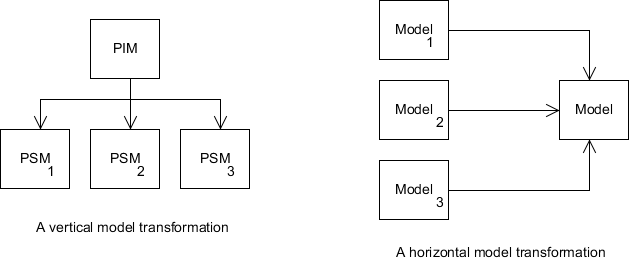
\includegraphics[scale=0.8]{./Figures/vertical_horizontal.png}
    \rule{35em}{0.5pt}
  \caption[Vertical and Horizontal model transformations]
  {Vertical and horizontal model transformations.}
  \label{fig:vertical_horizontal}
\end{figure}

The other provided example is a vertical model transformation that presents the
an example of an endogenous model transformation, that is refinement of a model.
If we do not consider the transformation that produces code, since this is an
exogenous model transformation. The three model types that MDA provides
can be viewed as a endogenous model transformation that provides a model that
is gradually refined into executable implementation code, by going through
refinement steps that add more details to the model. For example when mapping a
platform-independent model to a platform-specific model. Like we discussed in
section~\ref{MDA} a PIM describes the behavior and structure of an application
while a PSM describes all the information a specific technological platform
requires to implement the behavior and structure of this application. 

\section{Model Transformations in MDE}

Model transformations are in the center of Model Driven Engineering.
The vision for MDE is to increase automation of models between level of
abstractions. This vision is achieved through the use of model transformations.
Either if it is to use a model to text approach to generate source code, or by
transforming a model to another model where both models concrete syntax are
specified by an abstract syntax that a meta-model provides. A model driven
approach to software development thrives to keep a level of abstraction on the models for
as long as possible through translating these models. And therefore model
transformations are essential to be able to deploy model driven engineering in a
software development process. The principles behind OMG's Model Driven
Architecture utilize the concepts behind model transformation to a full extend. 
Figure~\ref{fig:MDE_MDA_MT} gives a representation of how MDA wishes to
facilitate the use of models and model transformations in a software
development. The figure was published in Kim Letkeman article, ``Comparing and
merging UML models in IBM Rational Software
Architect''\cite{letkeman2005comparing} in October 2010.

\begin{figure}[H]
  \centering
    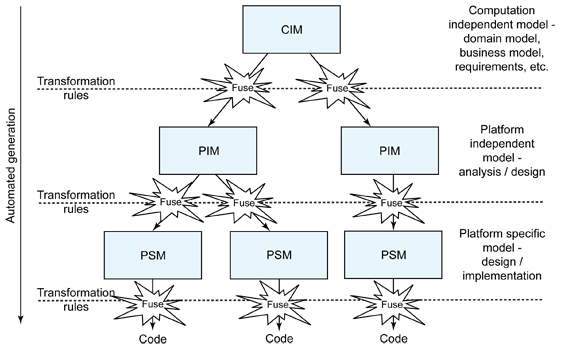
\includegraphics[scale=0.8]{./Figures/MDA_MDE.png}
    \rule{35em}{0.5pt}
  \caption[Model Transformations in MDA]
  				{Model Transformations in Model Driven Architecture.}
  \label{fig:MDE_MDA_MT}
\end{figure}

We can see the different level of abstractions that the architecture provides
and how to translate between abstractions. Remember what we discussed in
section~\ref{MDA} that the architecture represents a software design approach
for developing software applications. Where it expands the requirements of
a software application into models and at the last level of abstraction the
architecture provides implementation code for the application. The code that is
generated most likely requires some additional work by developers, but a major
part of the implementation code is generated through the use of models.
Figure~\ref{fig:MDE_MDA_MT} explains that a set of transformations are required
for a model to fuse to another model, or said differently, for a model to be
integrated into another model. These transformation rules, that specifies how a model from
a high level of abstraction is translated to a model on a lower level of
abstraction, provides a development process that produce implementation code
through automatically generating models on different levels of abstraction.
Models and model transformations are equally important for MDE to be applied in
a software development process. Without model transformations models would only
represent an abstraction of a system. This means by utilizing model
transformations in a software development cycle, models can evolve into
executable implementation code by translating through different level of
abstractions. 



%-----------------------------------
%	SUBSECTION 2
%-----------------------------------

\section{Classification of a model transformation}

In March 2006 Krzysztof Czarnecki and Simon Helsen published a domain analysis
to existing model transformation approaches\cite{Czarnecki2006}. A domain
analysis represents information on software system that share a common set of
features for a given domain\cite{FODA,Prieto-Diaz1990}, in this case the domain
is model transformations. This section is based on the ideas and results from
Czarnecki and Helsen's report. In their paper they presents the result by using
feature diagrams, that provides a terminology and representation of the design
choices for existing model transformation approaches. These feature diagram does
not only represent model to model transformation approaches, but also consider
the design choices for model to text transformation approaches. For the purpose
of this thesis we will only address the model to model approaches in Czarnecki
and Helsen's survey on model transformations. However it is important to
address that at top level, we can divide model transformations into to
categories, namely model to text and model to model transformations. The major
difference between these categories are that model to model transformations
generate a target model as an instance of the targets meta-model. While the
target of a model to text transformation are string sequences. Model to text
transformation are also often referred to as model to code transformation since
a collection of strings can be source code that corresponds to some programming
language. In this section we also consider the taxonomy of model
transformation\cite{Mens2006} that was published by Tom Mens and Pieter Van Gorp
in 2006. 

\begin{figure}[H]
  \centering
    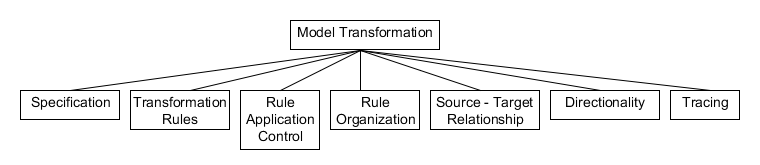
\includegraphics[scale=0.7]{./Figures/Model_Transformation_Survey.png}
    \rule{35em}{0.5pt}
  \caption[Domain Analysis of Model Transformations]
  				{A domain analysis of model transformations\cite{Czarnecki2006}.}
  \label{fig:Model_Transformation_Survey}
\end{figure}

Figure~\ref{fig:Model_Transformation_Survey} shows the feature diagram at top
level of a model transformation, where each subnode represents a major aspect
of model transformations. These major aspects of a model transformation can
give a better understanding on the different parts that a model transformation
provides. A model transformation requires that aspects from
figure~\ref{fig:Model_Transformation_Survey} is implemented in some manner.
Because the categories represents parts of a model transformation that in its
own way

%\subsection{Specification}

\subsection{Transformation Rules}

\begin{figure}[H]
  \centering
    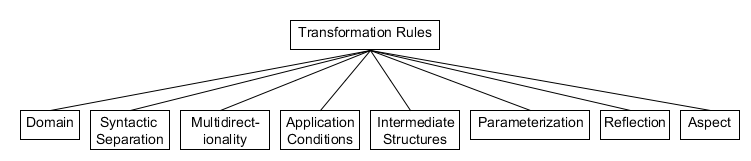
\includegraphics[scale=0.7]{./Figures/TransformationRules.png}
    \rule{35em}{0.5pt}
  \caption[Feature diagram for transformation rules]
  {Features for transformation rules.}
  \label{fig:TransformationRules}
\end{figure}

For a model transformation to be able to translate a model to another model it
needs a set of guidelines on how to achieve this. Therefore a model
transformation has a set of transformation rules that specifies how a target
model is produced. A transformation rule usually defines two special patterns.
One pattern represents a searching pattern while the other pattern represents
the part that is produced.  An obvious example of such rules are the rewrite
rules, that provides a left hand side (LHS) and a right hand side(RHS) where
both sides represents some user created patterns that are considered when a
transformation engine applies a corresponding transformation rule. But a
function that implements some transformation steps can also be seen as a
transformation rule. Regardless if the concrete syntax is either textual or
graphical, the users have to specify a pattern that is used to locate matches
and a pattern that is used to replace these matches with a result.

\textbf{Domain}

A transformation rule is specified by certain domains. These domains are
responsible of accessing either the source or target model for each
corresponding rule. A domain represents both the part that is used to find
matching patterns in a source model and the part that produces a target model.
For example for a classic rewriting rule we would have one domain for the LHS
and one domain for the RHS of the rule. 

\begin{figure}[H]
  \centering
    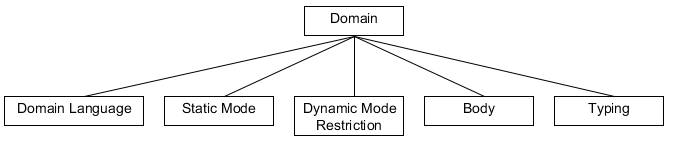
\includegraphics[scale=0.7]{./Figures/Domain_2.png}
    \rule{35em}{0.5pt}
  \caption[Feature diagram a domain]
  {Features for a domain.}
  \label{fig:Domain}
\end{figure}

Figure~\ref{fig:Domain} gives a representation of what a domain contains. A
domain is provided with a \textbf{domain language}. The domain language
represents how we can structure the domains. In the context of model
transformation tools that translates models that utilize the Model Driven
Architecture this domain language would have form of a meta-model expressed in
the Meta Object Facility. The domain language express what language we use to
define the abstract syntax for both the source and target model. \textbf{Static
mode} determines if a domain represents a searching part, a create target part, 
or as both. The classic rewrite rules has a source domain that represents the
LHS and a target domain that represents the RHS. Transformation rules that can
be applied in both directions assumes all domains to be both a source and a
target domain. \textbf{Dynamic mode restriction} concerns model transformation
tools that provides rules in multiple directions, that means that the source
and target model can act as both a source or target model depending on what
direction a transformation occurs. For these rules a domain can be restricted to
act as a source domain, and not as a target domain. A \textbf{body} determines
the actual pattern for a domain. This pattern has a certain structure, where the
pattern for example can represents graphs or strings. This pattern has a
provided abstract or concrete syntax. The abstract syntax describes what
modeling elements a certain pattern can contain while the concrete syntax
determines if the modeling elements are textual or graphical. The body part of a
domain can also contain logic that express computations and constraints on
modeling elements. \textbf{Typing} determines the typing of the contents of a
body. Patterns can either be untyped, syntactically typed or semantically typed.
For syntactically typing modeling elements that are part of a pattern is
associated with a meta-model element.  

\textbf{Syntactic Separation}

Some approaches to model transformation includes syntactic separation of
accessing models. These model transformation approaches clearly separates on
what models a transformation rules operates. For example in rewrite rules the
LHS operates on the source model while the RHS operates on the target model.
Some model transformation approaches might not have any distinctive separation,
like for example an model transformation implemented as a Java program. 

\textbf{Multi-directionality}

Multi-directionality determines if model transformation approach provides
transformation rules to be applied in different directions. This is convenient
when synchronizing models over model transformations for example. Model
transformation approaches that supports applying rules in both directions are
usually defined over a domain that is both a source and a target.


\textbf{Application Conditions}

\textbf{Intermediate Structures}

Some model transformation approaches requires intermediate structures when
executing a set of transformation rules. These structures are usually only
used as a supplement when applying a set of transformation rules. One
example of an intermediate structure is a traceable link. These traceable links
usually has a corresponding meta-model that is required to be included in a
model transformation environment. Some approaches to model transformation rely
on this intermediate structure to be able to translate a model. An example to
this is that this traceable link is created after a rule is applied to prevent
this rule for locating the exact same match next time it is applied. 

\textbf{Parameterization}

Parameterization allow for passing values to a transformation rule. For example
we can pass data types, for example modeling elements to a transformation rule.
We can then apply changes to a transformation rule with these provided
parameters and at the same time use the same data types in other
transformation rules.

\textbf{Reflection}

\textbf{Aspect}



\subsection{Rule Application Control}

This section can be divided into two sub categories, namely locating matches for
a transformation rules and how these rules are be applied. Locating a matching
pattern in a source model is rarely controlled by the users. The different
model transformation languages utilizes optimized searching algorithms to
locate these matches, where a rule has to be applied to a specific location in
a source model. Usually there are more then one exact match for each rule, and
therefore a transformation engine has to consider that there are several
matches for a specific search pattern in a source model. There are multiple
different search algorithms for locating these matches, but these search
algorithms often have a common strategy to determining the application
locations. The locate matches strategies could be applied deterministically or
non-deterministically for example. It is important to differentiate between a
strategy and a search algorithm. A strategy implies how an algorithm for
locating matches is executed. An algorithm that is applied by a deterministic
strategy, given a particular source model, will always produce the same output.
For example for directed graphs a deterministic strategy could exploit some
graph traversal algorithms, such as Breadth-first search\cite{Dasgupta2006}
(BFS) or Depth-first\cite{Dasgupta2006} search (DFS). An algorithm that are
executed with a non-deterministic strategy on the other hand can experience
different behaviors on different runs. An example of a non-deterministic
strategy is \textit{one-point} application\cite{Czarnecki2006} and
\textit{concurrent} application. A \textit{one-point} application applies a
rule to a non-deterministically location in a source model. This means that a
rule will search for matches at random locations within a given source scope.
While a \textit{concurrent} application applies a rule to all matching
locations at the same time. 

Before a matching pattern can be located in a source model a model
transformation environment has to have a mechanism that schedules these
transformation rules. Some model transformation tools provides the user with the
possibility to explicitly decide when transformation rules are applied. The
scheduling of transformation rules can be divided into implicit or explicit rule
scheduling. For an implicit rule scheduling mechanism the user are not given any
control over how transformation rules are applied, that is controlled by the
tool it self. Explicitly controlling the rule schedule can be achieved either
internal or external. Internal rule scheduling allows a transformation rule to
invoke other transformation rules, for example lazy rules in ATL. External
rule scheduling provides a mechanism that can include transformation rules and
execute these by some scheduling logic, for example sequentially executing a
collection of transformation rules. We can also select specific rules and
execute these accordingly. This is achieved by providing a scheduling mechanism
with a explicit condition that specifies how the transformation rules is
applied. This condition could for example specify that we should apply rules
according in a certain priority. A scheduling mechanism is then provided
with rules that is applied in priority over other rules. Now we have seen that a
scheduling mechanism can be defined explicitly or implicitly by the users and
can have conditions that determines if the rules should be applied in a certain
order. Model transformation tools also have scheduling mechanisms that provides
the possibility to iterate through a set of rules. What we mean by iterating
through a set of rules is that a model transformation tools applies a
transformation rule until there are no more matches. These rule iteration
scheduling mechanisms include recursion, looping and a fixed number of
iterations.

The available model transformation tools provides different solutions to both
locating matches and defining rule scheduling mechanisms. Usually the users are
given more freedom to defining the rule scheduling mechanism compared to
locating matches.

\subsection{Rule Organization}

This feature represents how the rules are organized and if they are easy to
reuse. The rules are usually represented as a collection of rules, where these
rules could either be represented in some source code or by some tree based
editor. Some model transformation approaches offer a modular approach to rule
organizing. This means that the rules are contained in a module and are
therefore easy to reuse. This gives the users the possibility to import these
modules and use them in other modules. This modular approach to creating
transformation rules can implement lazy rules, and lazy rules are transformation
rules that can be integrated in other rules. These rules are highly reusable and
can be used in any other module. In graph based model transformations rules are
in most cases organized into a set of rules, where each rule is not available
for other rules to use. This is because a transformation rule expressed in an
algebraic approach to model transformation has the pattern and the replacement
graph. And by adding a new rule with a new pattern graph and replacement graph
will probably result in a transformation rule that search for matches that was
not intended. 

\subsection{Source - Target Relationship}

How can a model transformation environment distinguish if a model
transformation is an endogenous or exogenous model transformation? This is
achieved by specifying how a source model and target model are related to one
another. These source and target models can relate to a meta-model for example.
Both the source and target model could be described by the same modeling
language. This specifies that a translation between source and target model are
an endogenous model transformation. And as we described in earlier in this
section is that an endogenous model transformation translates one model written
in one modeling language and produces a model written in the same modeling
language. One aspect of this source-target relationship is that the source and
target model are independent of each other. The model transformation
environment is responsible to read and write these models, and to make sure that
these models remain consistent. One could say that the target model are
implicit depending on a source model, since a model transformation requires a
source model to translate accordingly. The model transformation language creates
transformation rules based on the corresponding meta-models that describes both
the source and target model. And therefore administrate how these models relate
to one another through these transformation rules. If the source and target
models are written or modelled by using two different modeling languages, then
we have an exogenous model transformation, and the relationship between the
models should be adapted accordingly.

The source and target model can also in some cases be one and the same model,
Model transformations that are applied one and the same model are called
in-place model transformations. In AGG the source and target model are always
the same model, and therefore AGG only supports in-place update of a model.
The older versions of Atlas Transformation Language (ATL) requires that a new
target model, that is separated from a source model is created when applying a
model transformation. Creating a new model as a target model for a model
transformation specifies that this is an out-place change to a model. However
since January 2013 ATL support in-place transformations through a refining
mode. Other approaches offers support for both in-place or out-place updates
and lets the users specify how the models should be updated. These out-place
model transformations could either be changes made to an existing model or by
creating a new model. QVT Relations and Henshin is an example of approaches to
these model transformations. Henshin does implicitly deliver an in-place model
transformation environment, that allows for in-place update of models. But
explicitly, when using the Henshin API, one could programmatically set up
Henshin to do out-place changes to a model.

\subsection{Directionality}

This section describes that a model transformation environment can translate a
model in multiple direction. We can distinguish the direction model
transformations to either be unidirectional or multidirectional. An
unidirectional model transformation has one source model that translates to a
target model or updates a target model. What we then can do is change the source
model and source meta-model with the target model and target meta-model. But
this model transformation is not multidirectional, since we have to apply two
model transformation to achieve this. A multidirectional model transformation
can translate in different direction, regardless of source and target
meta-model. This is especially convenient for model synchronising, where we can
translate in multiple directions. 

\subsection{Tracing}

Some model transformation environment has support for tracing of model
elements. Tracing works like a fingerprint in a model transformation and
has an unique link between elements. A traceable link between source and target
elements is a link between mapped elements when a model transformation is
executed and provides information between the relationship between source
element and its corresponding target elements. The traceable link is stored in
memory for the duration it takes to execute a set of transformation rules. A
traceable link is specified when creating the transformation rules and requires
source and target elements. When there is a match in a transformation rule, a
new traceable link is created between a matched source element and all
corresponding target elements. These traceable links is very convenient when
analysing and debugging a model transformation. Because now there is tracing on
source and target elements on each time a transformation rule finds a match in
the source model.

How traceable links are used across transformation tools varies. In Henshin, ATL
and QVT these traceable links are handled automatically. For Henshin the user
can use Henshin Trace model to create traceable links. The trace model consists
of a single class Trace with a source and target reference. The user can then
create this trace element together with the transformation rules to relate
source and target models. ATL has an implicit tracing mechanism that specifies
relationships between the source element and its corresponding target elements
by using a native type called ASMTransientLink\cite{Wagelaar}. For every time a
transformation rule is matched to a source element, one ASMTransientLink is
created. To this transient link the name of the transformation rule provided
together with the source element and the target elements. These links are added
to a collection that has all the transient links and stored internally for ATL.
This means that the users of ATL cannot access these links after a model
transformation has finished executing. However, as shown by Andr\'{e}s Yie and
Dennis Wagelaar\cite{Wagelaar}, that gaining access to these ATL traces can be
done explicitly by creating transformation rules that generates a tracing
model based on the internal tracing information provided by ATL. In AGG
traceable links are created as any other modeling element. Where the user can
specify a node and two arrows between source and target meta-element in the type
graph. 

%----------------------------------------------------------------------------------------
%	SECTION 2
%----------------------------------------------------------------------------------------

\section{Graph based Approach to Model Transformations} 
\label{sec:graph_based}

One common approach to model transformations is by graph transformations,
also referred to as graph rewriting. Graph rewriting can be implemented with
an algebraic approach, which is based on Category Theory. Before we go into
detail about graph transformation, we should quickly describe the concepts of
Category Theory\cite{Herrlich1973,Barr1990}. Category theory can be used to
formalize mathematical or software theory's at a high level of abstraction. In
2006 Steve Awodey published a second edition of the book, Category Theory,
where he stated,

``Just as group theory is the abstraction of the idea of a system of
permutations of a set or symmetries of a geometric object, category theory
arises from the idea of a system of functions among some
objects\cite{Awodey2006}.''

\begin{figure}[H]
	\centering
	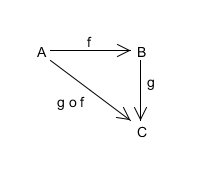
\includegraphics[scale=0.7]{./Figures/categoryTheory.png}
	\caption[Category Theory]
	{Collection of objects A,B and C.}
	\label{fig:categoryTheory}
\end{figure}

Category Theory can be used as a supplement to explain the theoretical aspects
behind a problem or solution. A category consists of a collections of
objects and functions. In figure~\ref{fig:categoryTheory} we have a collection
of objects A, B, C and arrows f, g, g $\circ$ f. The figure describe that
there is a connection between the two objects A and B. This connection
indicates that there are some association between two objects. For this case
this means that function f is defined in A and the values of this function are
in B. When the objects represents graphs, then these connections between objects
are often referred to as morphisms between graphs or graph morphisms. Morphisms
are pair of maps which commute with source and target\cite{Brown2008}.
Figure~\ref{fig:categoryTheory} has three sets of graph morphisms, f : A
$\longrightarrow$ B, g : B $\longrightarrow$ C and g $\circ$ f : A
$\longrightarrow$ C. The last set of graph morphisms, g $\circ$ f indicates that
there is a composite function between A and C. This basically means that if
C is a function g of B and B is a function f of A, then C is the result of a
function between C and A. 

For the purpose of this thesis the collection of objects represents graphs the
arrows represents morphisms. A graph contains a collection of nodes and edges.
A graph is undirected when there is no distinction between two nodes associated
with an edge or it is a directed graph if an edge has a direction between two
nodes. This means that each node is represented as a source and a target node
for an edge. A directed graph L can be defined by L = \{
N\textsubscript{L}, E\textsubscript{L}, source\textsubscript{L},
target\textsubscript{L} \}. N\textsubscript{L} represents the collection of
nodes and E\textsubscript{L} represents the collection of edges that are
included for the directed graph. The third and forth elements,
source\textsubscript{L} and target\textsubscript{L}, are functions that
retrieves the source and target node for an edge. This collection of nodes and
edges in a graph L can result in an excact match in another graph G. The
morphism between these two graphs are called homomorphism.

\subsubsection*{Graph Homomorphism}

When a graph that has a mapping of nodes and edges in another graph, then there
is a graph homomorphism between these two graphs.

\begin{figure}[H]
	\centering
	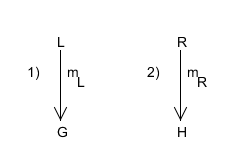
\includegraphics[scale=0.7]{./Figures/GraphHomomorphism.png}
	\caption[Basic concepts of graph homomorphism]
	{Two sets of graph homomorphism of graph L in G and R in H}
	\label{fig:graphHomomorphism}
\end{figure}

Figure~\ref{fig:graphHomomorphism} has two graph homomorphisms
\mbox{L$\xrightarrow{m\textsubscript{L}}$G} and 
\mbox{R$\xrightarrow{m\textsubscript{R}}$H}. Now if we consider the first
example, if there is to be a valid graph homomorphism between graph L and G,
then the collection of nodes and edges in L has to be mapped to nodes and edges
in G. If both graphs L and G are directed graphs we can safely assume that the
definition of graph L in the last paragraph is also true for graph G =\{
N\textsubscript{G}, E\textsubscript{G}, source\textsubscript{G},
target\textsubscript{G} \}. For a graph homomorphism m\textsubscript{L} from the
graph L to the graph G, \mbox{L$\xrightarrow{m\textsubscript{L}}$G}, there is a
mapping m\textsubscript{L} : N\textsubscript{L} $\longrightarrow$
N\textsubscript{G} from the set of nodes in graph L to the set of nodes in
graph G and a mapping mapping m\textsubscript{L} : E\textsubscript{L}
$\longrightarrow$E \textsubscript{G} from the set of edges in graph L to the
set of edges in graph G that preserve both source and target nodes. This means
that there is a mapping from a source node in G that is equal to a source node
in L and a target node in G is equal to a target node in L. 

\subsection{The Algebraic Approach}
This approach are based on the concepts of composing graphs, modelled
by pushouts of graphs and graph morphisms. This pushout approach comes in
different variants, and we will look at two of these, namely the
double-pushout (DPO) approach and the single pushout (SPO)
approach\cite{Loewe1997,Ehrig1997}.

Historically, the first of the algebraic approaches to graph
transformations, the double-pushout, was first introduced at the Technical
University of Berlin in the early seventies by H. Ehrig, M. Pfender and H.J.
Schneider\cite{INSPEC:606170}. They tried to generalize Chromsky grammars from
strings to graphs. This allowed to define a graph rewriting step by the use of
two gluing constructions. And by applying a graph rewriting step for the
double-pushout approach is a pair of morphisms in the category of graphs where
the arrows represents total graph morphisms, \mbox{L $\longleftarrow$
\ K $\longrightarrow$ R}. This is true for each application rule in a graph
transformation for the double-pushout approach. Where the graph K represents the
common part and the two morphisms \mbox{L $\longleftarrow$ \ K} and \mbox{K
$\longrightarrow$ R} use the algebraic construction, pushout to apply an
application rule for a rewriting step. Hence the name double pushout and the use
of two rewriting conditions.

\subsection{Transformation Rules}
For a transformation language to be able to execute graph
transformations a set of application rules needs to be defined. Through these
rules, a transformation interpreter can act accordingly. These rules can have
many names, and are often referred to as productions or applications. For graph
transformations, there can be an arbitrary number of rules. Its truly up to the
users how they want to translate a language and how many rules that is needed
to acquire this. Each rule consists of a left hand side (LHS) and a right hand
side (RHS), also often referred to as pattern graph and replacement graph. The
pattern graph represents a subgraph of the model that is going to be translated,
namely the host graph. For these productions to execute, there is an application
control mechanism that administrates the execution ordering of transformation
rules. 

\subsection{Application Control}
In graph transformation, there has to be a control mechanism that
administrates these productions. These control mechanisms are also called
transformation units. These units controls the order that the transformation
rules are executed. The most basic transformation unit is a rule itself which
corresponds to a single application of that rule. But in most cases, a
transformation unit will have to control several rule applications. 

\subsection{Execution of rules}
The basic idea for graph transformation for both the double-pushout
approach and the single pushout approach is to apply an application rule
\mbox{r: L $\longrightarrow$ R}. Where the rule represents a single rewriting
step for graph transformations and L represents the left hand side of the rule and R
represents the right hand side of the rule.

\begin{figure}[H]
	\centering
	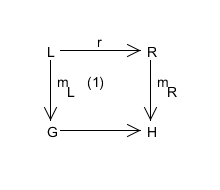
\includegraphics[scale=0.7]{./Figures/Single_Pushout.png}
	\caption[Idea of graph transformation]
	{The basic idea for graph transformation by applying a rule r.}
	\label{fig:GraphTransformationGeneral}
\end{figure}

A production rule r, \mbox{G$\xrightarrow{r,m}$G'} indicates a direct
derivation to a derived graph G'. In
figure~\ref{fig:GraphTransformationGeneral}, the graph G' is created by
applying a single pushout for a transformatin rule r. If there is a match m of
nodes and arrows for a subgraph L in a host graph G, Then this indicates a
graph homomorphism, mapping elements from the subgraph to the host graph in
such a way that the graphical structure in G is preserved. For each rule r,
there are some algebraic approaches to how we can achieve G'. At this moment
there are four approaches, the double-pushout approach (DPO) \cite{Loewe1997}, the
single-pushout approach (SPO) \cite{Ehrig1997}, the
sesqui-pushout\cite{Corradini2006} and the pullback approach\cite{Bauderon}.
Where the two most common approaches used in graph transformation tools are the
DPO and the SPO approach. There is one major aspect that separate these two
approaches, and that is that the DPO approach has an application condition.

\begin{figure}[H]
	\centering
	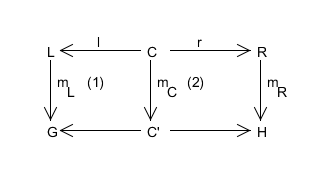
\includegraphics[scale=0.7]{./Figures/Double_Pushout.png}
	\caption[The Double Pushout approach]
	{Principles behind the double pushout approach.}
	\label{fig:DPO}
\end{figure}

\noindent This application condition, named the gluing condition\cite{Loewe1997}
consists of two parts. Namely the dangling condition and identification
condition. From figure~\ref{fig:DPO}, the dangling condition requires that if
the transformation rule p specifies the deletion of a node in G, then it must also
specify the deletion of all incoming and outgoing edges of this node in G. By
applying this condition, we can be sure that there are no dangling edges after
deleting a node in G. The identification condition requires that every element
of G that should be deleted by applying a transformation rule p is only present
once in L for each transformation rule p. 

A single transformation rule p in the DPO approach is given by a pair of graph
homomorphisms from a common graph C. This common graph C is formed by taking
elements that are present in both L (LHS) and R (LHS) of a transformation rule
p. The graph G' are created from the graph G, by deleting all elements that is
matched from the pattern graph L, but none in C. To avoid dangling edges,
the gluing condition must be satisfied before deleting these elements. This is
the first part (1) of the DPO approach, namely the deletion of elements. The
second part (2) is insertion of elements. From here we create a graph H off all
nodes and arrows from the replacement graph R that is not presented in the
common graph C. The DPO approach has the possibility to preserve elements from
translating from the pattern graph L and the replacement graph R with the help
of a common graph C.

For the SPO approach on the other hand, deletion has priority over preservation.
Figure~\ref{fig:GraphTransformationGeneral} is a representation of the practices
of the SPO approach. Where nodes that are present in the pattern graph L but not
the replacement graph R are deleted. And the incoming and outgoing edges of the
deleted nodes that are not present in the replacement graph R is deleted.

\begin{figure}[H]
	\centering
	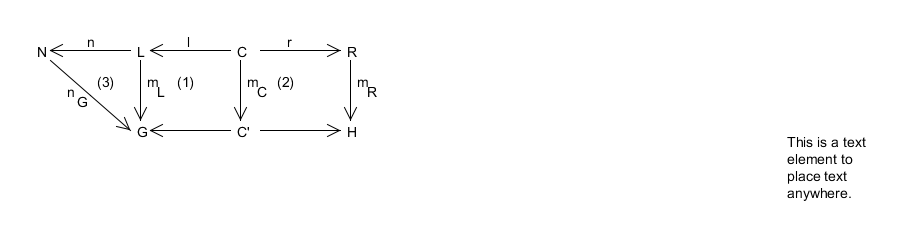
\includegraphics[scale=0.7]{./Figures/Double_Pushout_NAC.png}
	\caption[The Double Pushout approach with NAC]
	{Double pushout approach with negative application condition.}
	\label{fig:DPO_NAC}
\end{figure}

\begin{figure}[H]
	\centering
	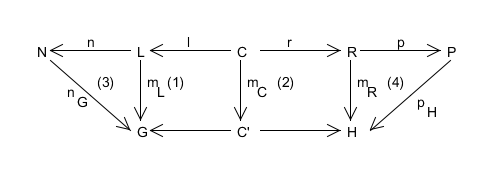
\includegraphics[scale=0.7]{./Figures/Double_Pushout_PAC.png}
	\caption[The Double Pushout approach with PAC]
	{Double pushout approach with positive application condition.}
	\label{fig:DPO_NAC}
\end{figure}

%\section{Hybrid based approach to Model Transformations}

%A hybrid bases approach to model transformation 




% Chapter Template

\chapter{Problem Specification} % Main chapter title

\label{Chapter4} % Change X to a consecutive number; for referencing this chapter elsewhere, use \ref{ChapterX}

\lhead{Chapter 4. \emph{Problem Specification}} % Change X to a consecutive
% number; this is for the header on each page - perhaps a shortened title

%----------------------------------------------------------------------------------------
%	SECTION 1
%----------------------------------------------------------------------------------------

\section{Problem Specification}
\label{problem}

The DPF Workbench already includes support for model transformations. However,
the framework does not have support for transforming a model between different
modeling langauges. One of DPF's strengths is that it is possible to formally
define a Domain Specific Modeling Language by defining multiple levels of
meta-models. What we want to do is to include tool support for the DPF Workbench
that change a model from one meta-modeling hierarchy to another meta-modeling
hierarchy regardless of the source models abstraction layer. This leads to the
main question for this thesis.

\begin{itemize}
  
  \item Can we include tool support for model to model transformations for the
  DPF Workbench that translates a model specified over a modeling hierarchy to a
  model specified over another modeling hierarchy?

\end{itemize}

The solution to this is not written in stone, and there are several approaches
to how we can solve this specific problem. The tool requires some implementation
but there are several existing approaches available that provides model
transformations as we mentioned in section~\ref{tooling}. DPF specifications are
basically graphs, more specific, they are directed graphs. This means that a
DPF specification consist of a set of nodes, arrows and two functions that
preserves the source and target node. This makes a graph based approach to model
transformations convenient, but we should also consider other approaches to
model transformations. 

\begin{itemize}
  
  \item Can we integrate an existing model transformation environment with the
  Diagram Predicate Framework Workbench?

\end{itemize}

We want to introduce the DPF Workbench with tool support that includes model
transformations. This has already been successfully introduced to the workbench
environment in Anders Sandven\cite{Sandven_thesis}'s master thesis. In his
thesis he describe how he integrated a M2T transformation environment to the DPF
Workbench. He integrated a model transformation environment, Xpand\cite{Xpand}
that provides a template based approach to Model2Text transformation. For this
thesis however, we want to verify that we can successfully introduce a model
transformation environment that supports translation between different DSML's.
But first we have to find a applicable environment that can be integrated with
the DPF Workbench. In section~\ref{tools} we will explore three different
model transformation tools that supports both exogenous and endogenous model
transformations. One aspect of model transformations that is required to
translate specifications in DPF is a set of transformation rules that describes
how a target model is produced. This leads to a problem for the DPF, because a
transformation rule requires modeling elements from some abstract syntax to
specify a structural pattern that is used to locate matches in a source model. 

\begin{itemize}  

  \item How can we include the abstract syntax of a modeling language that is
  specified to a corresponding linguistic meta-model and an corresponding 
  ontological meta-model for a single transformation rule.

\end{itemize}

In 2007 Ralf Gitzel, Ingo Ott and Martin Schader published a paper where they
amongst other subjects discuss the difference between Linguistic and
Ontological meta-modeling. They provide a definition between the two, 
\textit{``Linguistic metamodeling uses a metamodel to describe a language syntax
without a concrete real-world mapping. Ontological metamodeling uses metamodels
to describe domain-specific hierarchies"}\cite{gitzel2007ontological}. As it is,
the MOF 2.4.1 standard does not allow for more than a four layered
meta-modeling. DPF has an Ecore specified meta-model that describes the
language syntax and potentially unlimited layers of meta-models that describes the
domain-specific hierarchy. Figure~\ref{fig:core_metamodel} gives a
representation on how specifications are related and regardless of abstraction
layer every specification $\spec{S}$\textsubscript{1\ldots n} conforms to one
common meta-model.

\begin{figure}[H]
	\centering
	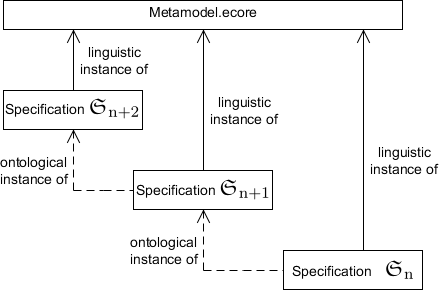
\includegraphics[scale=0.7]{./Figures/metamodelSpecification_1.png}
	\caption[Specification relationship with core meta-model]
	{Relationship between layers of DPF specifications.}
	\label{fig:core_metamodel}
\end{figure}

This model is the linguistic meta-model that DPF provides to describe the
abstract syntax for every single specification created by the DPF Model Editor.
However, other than consisting of an underlying graph and a set of constraints,
a DPF specification $\spec{S}$\textsubscript{n} is also an instance of another
specification$\spec{S}$\textsubscript{n+1}, and this is where it gets
challenging. Because in the DPF Workbench a specification model
$\spec{S}$\textsubscript{n} is created as an instance from a specification model
$\spec{S}$\textsubscript{n+1}. We can describe these specification models as
ontological meta-models, since these models describes a domain specific modeling
language through an arbitrary hierarchy of models. This is where we have to find
a work around for our solution, because model transformation environments that
utilize Ecore based models does not allow Ecore instance models to represent
abstract syntax. This could serve a potential problem when integrating the model
transformation environment with DPF. Modeling elements that DPF provides are
created as nodes and arrows from an Ecore based meta-model, but are at the same
time created according to modeling elements one abstraction layer higher.

We will discuss how we address and approach these problems in the next
chapter. But first we will look at some related work to model transformations.
We have considered the tools, The Attributed Graph Grammar
System\cite{Taentzer2004} (AGG) and Henshin\cite{Henshin_2010} that provides a
graph based approach to model transformation. We have also worked with ATLAS
Transformation Language\cite{ATL_USERMAN} (ATL), that provides a mixture of
model transformation techniques and is therefore often referred to as a hybrid
approach to model transformation. Through working with these three tools we can
find a model transformation environment that is best suited to be integrated
with the DPF Workbench.

\section{Three different model transformation environments}
\label{tools}

These model transformation tools use different approaches to how model
transformations are applied. We have looked at tools that implement classical
rewriting steps that utilizes the theory behind graph transformations and tools
that does this differently. For this survey we have tackled a specific
exogenous model transformation example, that translates an instance model of
UML's activity diagram to an instance model of a Petri
Nets\cite{jensen2007coloured} model. The next two figures provides the abstract
syntax of the two corresponding languages. These figures are represented as
Ecore models, that is EMF's interpretation of OMG's MOF. It is convenient to
represent these meta-model as Ecore models since both Henshin and ATL specify
transformation rules according to such models. First we will quickly describe
the corresponding abstract syntax for the two models before we consider the
first model transformation tool.

\begin{figure}[H]
	\centering
	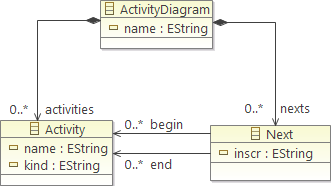
\includegraphics[scale=0.7]{./Figures/ActivityMetamodel.png}
	\caption[Abstract syntax of the source model]
	{Abstract syntax of the source model for this test case.}
	\label{fig:activity_metamodel}
\end{figure}

The abstract syntax for the source model has an arbitrary number of
activities and next elements. Figure~\ref{fig:activity_metamodel} describes that an activity
element can have a name and a kind. The next element can have an inscription
and provides the property to either begin or end activities. The collection of
activities and next elements are provided by a specific activity diagram that.

\begin{figure}[H]
	\centering
	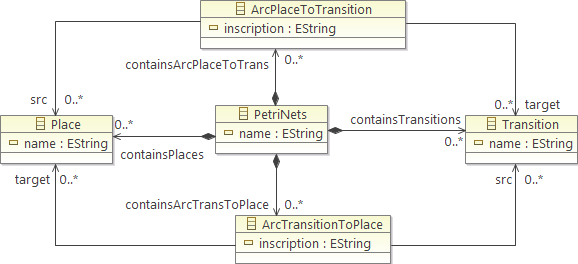
\includegraphics[scale=0.7]{./Figures/PetriNetsMetamodel.png}
	\caption[Abstract syntax of the target model]
	{Abstract syntax of the target model for this test case.}
	\label{fig:petrinet_metamodel}
\end{figure}

The abstract syntax for the target model consist of places and transitions. A
Petri net instance must have a place connected to a transition or the other way
around, but a Petri net model can never have two of the same types connected.
For this test case we defined two nodes that specify if a connection is between
a place and a transition or a transition and a place. Note that these two
meta-models are a simplified version of the abstract syntax. For this test case
we are more concerned with how the different model transformation environments
refers to the abstract syntax for the transformation rules. For each tool, if it
is either a graphical editor or a textual editor, we discuss how to edit
transformation rules, which is relevant for how we want to design a
transformation tool for the DPF Workbench. We then consider how the different
tools defines the abstract syntax for both the source and target model. Next we
specify how transformation rules are created and if the tool provides any
application control for these rules. We finish up by mentioning how the tool
applies this model transformation. In section~\ref{tool_choice} we consider the
model transformation environment that can be integrated and provides a viable
model transformation technology that works with the DPF Workbench.

\subsection{The Attributed Graph Grammar System}

AGG is a general development environment for algebraic graph
transformation systems that provide a graphical editor for creating
and modifying graphs. The editor provides a graphical user-interface with
several visual editors for applying the principles of graph transformations. AGG
also provide an interpreter and a set of validation tools. The system is an
ongoing research activity of the graph grammar group at TU Berlin and started
in 1997.

\subsubsection*{Graphical Editor}
The graphical editor of AGG, represented in figure~\ref{fig:AGGScreen}, has
several functions to help the user to define model transformations. In the top
left corner of the graphical user-interface is a tree based editor that provides
a set of transformation rules, type graphs, and host graphs. The host graph
represents both the source and target model in a model transformation, and the
type graph represents the abstract syntax for the modeling languages. The
source-target relationship of the host graph is one and the same, but we will
discuss this in future sections, but for the purpose of this thesis we will
refer to the host graph as the source graph.

Each transformation rule has two visual editors, representing the left
(LHS) and the right hand side (RHS), or the pattern and the replacement graph.
In the tree based editor it is also possible to attach application conditions to
transformation rules. This is convenient if the user wants to specify
constraints that restricts the pattern or replacement graph to be applied
accordingly to the specific application condition.

Type graphs are described more in depths in the next section, but roughly said,
the type graph defines modeling elements that can be used to create the source
graph and is similar to how Ecore defines meta-models for EMF. The users can
now create model instances that represents the concrete syntax of a specific
modeling language. This representation of the abstract syntax are represented
in a source and corresponds to its concurrent type graph.

The transformation rules can be extended with Java expressions. This means that
the users can use Java primitives such as strings, integers or float numbers to
form the pattern graph or the left hand side of the rule. However, the users
can only bind attributes that are in a corresponding type graph.

Figure~\ref{fig:AGGScreen} also represents some node elements and association
elements. These are meta elements that are initialized in the type graph and
are used to model the source graph, the different transformation rules and
application conditions. The node elements and association elements also
describes the semantics of the type graph. Note that both the node elements and
association elements in the figure has been scaled up for the purpose of this
paper.

\begin{figure}[H]
  \centering
    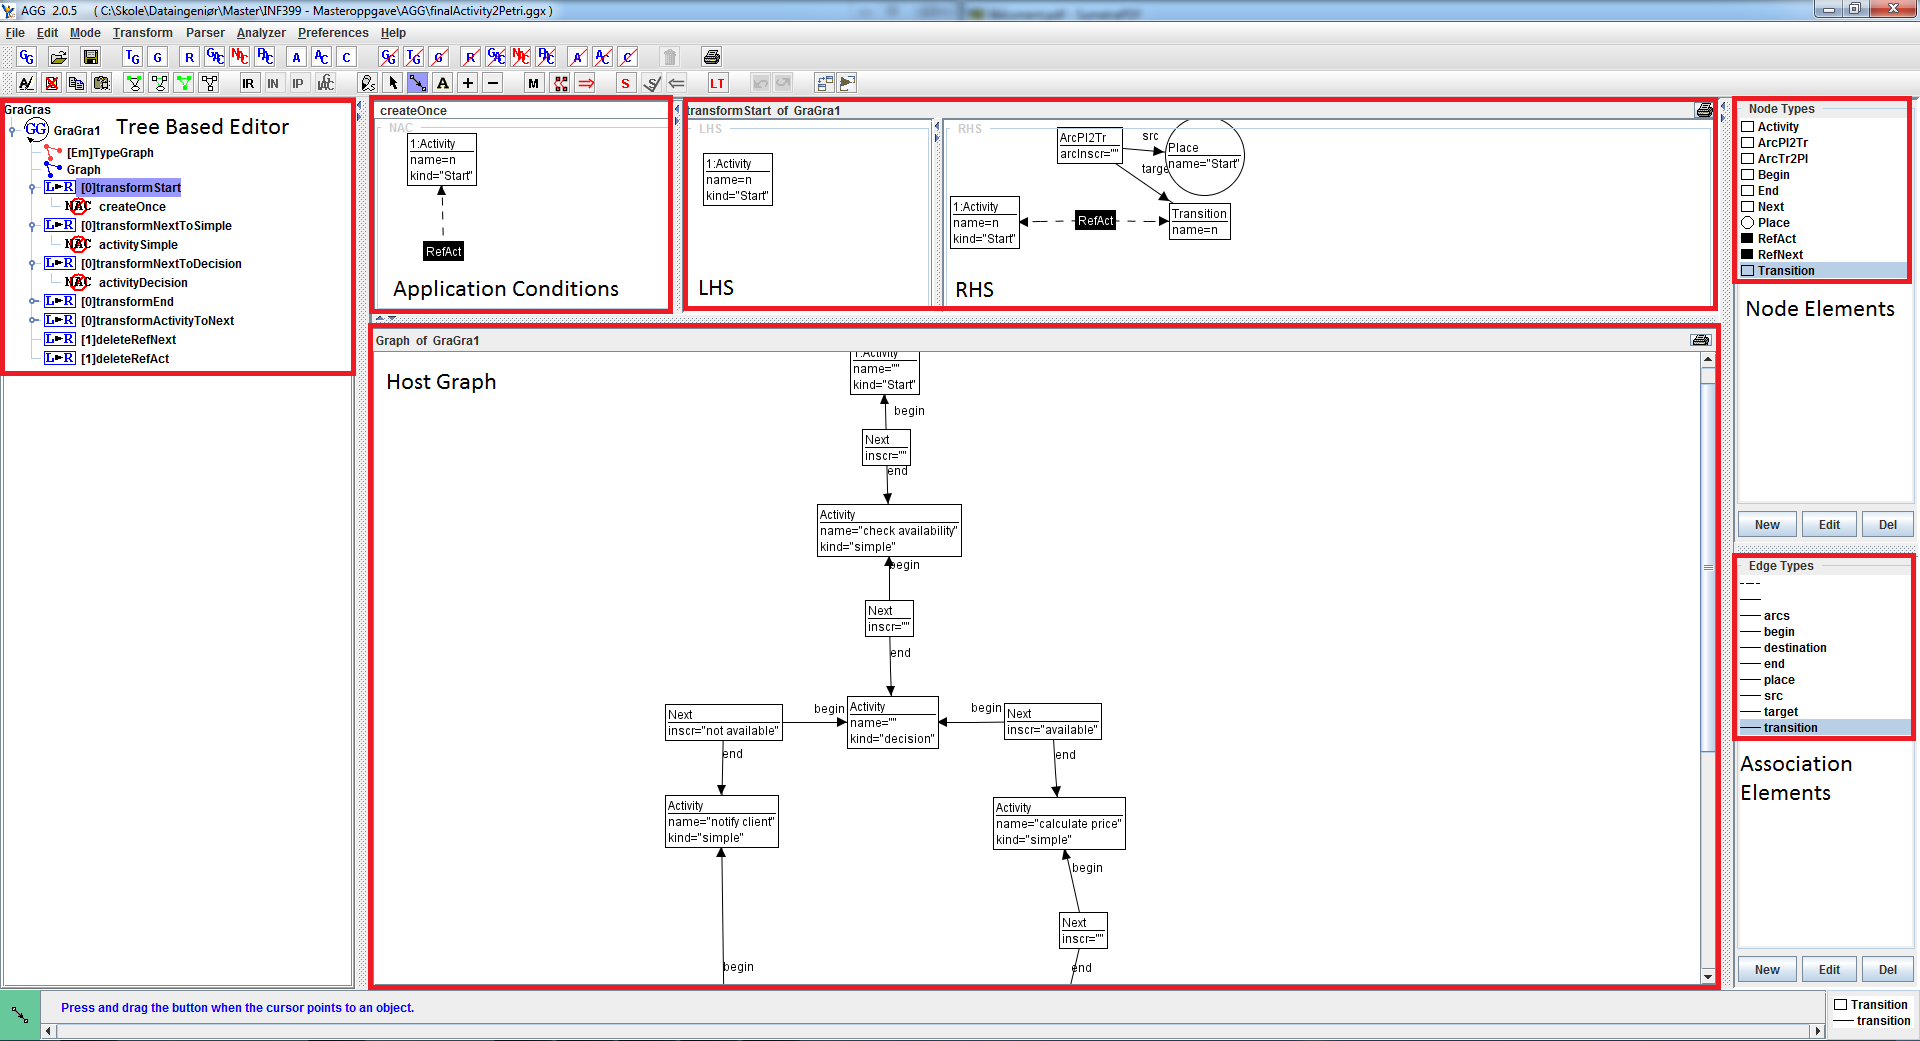
\includegraphics[scale=0.3]{figures/AGGscreen.png}
    \rule{35em}{0.5pt}
  \caption[Graphical Editor for AGG]
  {A model transformation for the AGG Editor.}
  \label{fig:AGGScreen}
\end{figure}

\subsubsection*{Defining Meta-models}

Before the source graphs can be created, we have to specify the modeling
language for the source model and the target model. In AGG both the source and the
target meta-model are defined in one common type graph. The type graph
represents the abstract syntax for both the source and target model. If we want
to prepare an AGG graph for a model transformation, we create a type graph with
references between source modeling elements and target modeling elements. AGG is
unaware of the relationship between these modeling elements unless we explicitly
initialize them. The relationship between source and target modeling elements in
the abstract syntax has two major purposes for an exogenous model
transformation. The relationship specifies how source modeling elements
correspond to target modeling elements and determines upon execution of
transformation rules that a matched pattern is only found once. 

\begin{figure}[H]
	\centering
	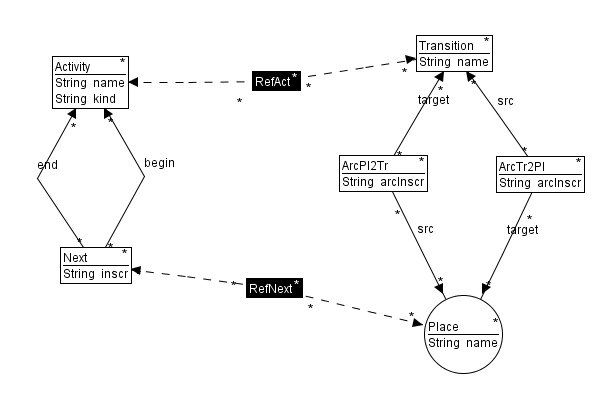
\includegraphics[scale=0.7]{figures/AggTypeGraph.png}
	\rule{35em}{0.5pt}
	\caption[Type graph in AGG]
	{Type graph for activity diagram and Petri Net in AGG.}
	\label{fig:AggTypeGraph}
\end{figure}

Figure~\ref{fig:AggTypeGraph} represents the type graph for our test case. The
abstract syntax contains nodes and arrows that include a structural multiplicity
constraint. The user defines nodes and arrows for each meta element for both
the source and target model. This is achieved by using either the Edge Type
Editor or Node Type Editor and are editors that correspond to either a node or
an edge. The nodes and edges are given names and graphical properties such as
colors or shapes. Nodes represents modeling elements from the two modeling
languages while arrows represents the associations between these modeling
elements. In the type graph we want to distinguish between associations and
correspondences, and therefore we represent a correspondence between a source
and target modeling element as a dashed arrow. The dashed arrow has the same
properties as the association arrow between nodes, but the graphical
representation is different. This makes the concrete syntax in the source graph
easier to read when we are applying the transformation rules. In
figure~\ref{fig:AggTypeGraph} we can see that a RefAct node is defined and is
connected between the activity element and the transition element. The same
initialisation is defined between the next element and the place element. This
reference edge specifies that there is a correspondence between Activity and
Transition element and between Next and Place. For this type graphs there is a
structural multiplicity constraint for the nodes and edges. This means that
there can be an arbitrary, or a zero to many number of instances of these nodes
and edges in the source graph.

\subsubsection*{Defining Transformation Rules}
\label{sec:AGG_rules}
Now the type graph has been initialised and the instance graph of the
source model has been created. But to be able to translate to a target model,
we need to create a set of transformation rules. A transformation rule is
defined with an unique name, an empty LHS graph and an empty RHS graph. 

\begin{figure}[H]
	\centering
	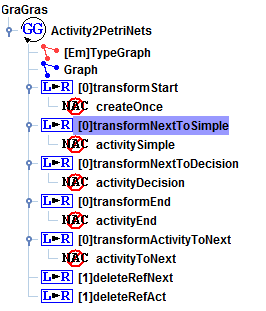
\includegraphics[scale=0.7]{figures/AGGTreeBasedEditor.png}
	\rule{35em}{0.5pt}
	\caption[Tree based editor in AGG]
	{Tree based editor for transformation rules.}
	\label{fig:AGGTreeBasedEditor}
\end{figure}

Whenever changes are made in the two graphs, AGG checks if the LHS or the RHS
conforms to the type graph. The user is unable to insert elements in the two
graphs that are not initialised in the type graph and the users are not allowed
by AGG to create associations between nodes that are not initialised in the type
graph. This is how AGG keep the source and target models consistent. In
figure~\ref{fig:AGGTreeBasedEditor} we can see the tree based editor in AGG,
that provides the type graph, the source graph and a list of transformation
rules. When a new rule is created, both the LHS and the RHS are initialised. The
users can then specify a graph structure that forms the LSH graph that AGG use
to locate matching patterns in a source graph. The RHS graph represents the
graph structure that the transformation system produces for each located match.
AGG provides two visual editors for these corresponding graphs. However, there
is also a graph that represents the intersection between the LHS and the RHS. In
AGG this graph is edited by creating similar modeling elements in both the LHS
and RHS graph and map these modeling elements with each other. 


\begin{figure}[H]
	\centering
	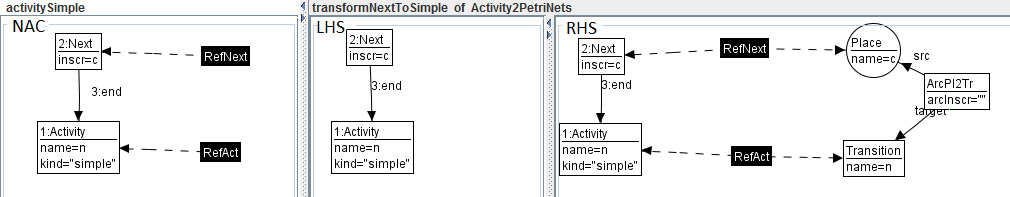
\includegraphics[scale=0.5]{figures/LHSvsRHSAGG.png}
	\rule{35em}{0.5pt}
	\caption[Representation of a rule in AGG]
	{The LHS and RHS of a rule and a NAC attached.}
	\label{fig:LHSvsRHSAGG}
\end{figure}

Figure~\ref{fig:LHSvsRHSAGG} is a representation of the rule
transformNextToSimple, with the LHS and the RHS graph. The LHS contains the
graph structure that is used to locate matches while the RHS contains the
graph structure that replaces the located matching pattern. For this rule the
modeling elements that are represented in the LHS are also part of the graph
structure in the RHS graph. Modeling elements that are part of both the LHS and
RHS graph can be mapped together to specify for a transformation engine that
these modeling elements defines a graph structure that is an intersection
between the LHS and the RHS graph. In section~\ref{sec:graph_based} we
introduced the concepts of single and double pushout of graphs for graph based
model transformation tools. A double pushout of graphs includes this
intersection graph for a transformation rule that makes it possible to preserve
modeling elements that is part of both the LHS and the RHS. Modeling elements
that is defined in the LHS graph and not the RHS graph are removed when the AGG
transformation engine applies a transformation rule. For example the
transformation rule in figure~\ref{fig:LHSvsRHSAGG} locates the graph structure
that the LHS defines in a source graph and inserts a new graph structure that
the RHS defines in the source graph. This transformation rule will not remove
any modeling elements once applied since we have specified that the modeling
elements that is part of the LHS graph are also part of the RHS graph. A rule
can also specify application conditions that can either be a Positive
Application Condition (PAC) or a Negative Application Condition (NAC).
Figure~\ref{fig:LHSvsRHSAGG} has a NAC, activitySimple that makes sure that the
LHS of the rule is translated only once for each pattern match found in the
source graph. This is because for each applied transformation rule we preserve
the LHS graph structure and therefore is a potential match the next time the
transformation rule is applied. However, the negative application condition
requires that the matching pattern should not contain any references and
therefore is not a valid matching pattern. Through the use of these application
conditions, the users can create restrictions to how each transformation rule
should handle matching patterns in the source graph. A transformation rule
can have multiple application conditions attached.

\subsubsection*{Application Control for the Transformation Rules}

In subsection~\ref{sec:app_control} we specified that the application control of
a model transformation handles the location of matches and rule application
control. Locating matches in AGG are designed by some non-deterministic search
algorithms that the users have no control over. AGG does however provide the
users with the possibility to explicitly specify how the transformation rules
are applied. By default, the transformation rules are applied
non-deterministically. This means that there are no pattern to how the
transformation rules are applied and the transformation rules can be applied
differently on different runs. This option is quite useful if the set of
transformation rules are independent of each other. AGG also provides other
ways of applying rules such as applying rules by layers or by sequences. When
the transformation is set to be applied by rule layers, then AGG introduce
the users with an integer that specify transformation rules on different layers.
This layer number will range from 0 \ldots n, where the lowest number is the
first layer and therefore the has first priority. If there are rules with
the same layer number, then these rules will be internally applied
non-deterministically. If the rules are applied by sequence then the rules will
be applied from the first element in the tree based editor and applying the rest
of the rules in sequence.

\subsubsection*{Translating the Source Graph}

In section~\ref{sec:AGG_rules} we described that when applying a transformation
rule a matching pattern is located in the source graph and a graph structure
from the RHS is inserted in the source graph. This is special source models in
AGG, because the source graph in AGG represents both the source model and the
target model in a model transformation. AGG's transformation system provides an
in-place model transformation directly on the source graph. An exogenous model
transformation that is specified in AGG usually include all located matches in
the translated graph structure for each transformation rules. These modeling
elements that represents the abstract syntax of the source model can then be
removed through a set of transformation rules after the modeling elements
that correspond to the abstract syntax of the target model is translated. This
means that for an exogenous model transformation we should be careful when
applying the transformation rules non-deterministically. The user can now
either press Start Transformation or do the transformation one step at the
time. For the first option AGG will apply one rule at the time until there are
no more matching patterns located in the source graph. When AGG cannot find
any more matches, the host graph is either correctly translated or there are
errors in the rules. The user can also execute the transformation step by step.
This will give the user the same result as the first option, but now the user
can do one match at the time for each rule. AGG utilize both the single and
double pushout approach when executing a transformation
rule\cite{Taentzer2004}. Like we discussed in section~\ref{sec:graph_based} the
single pushout approach removes the graph structure from the LHS and inserts the
graph structure from the RHS in the source graph. If the rules specifies an
intersection graph between the LHS and RHS graph then the double pushout
technique is used. AGG's transformation engine interpret a transformation rule
and applies the transformation rule accordingly. Another model transformation
environment that similar to AGG utilizes the concepts of graph transformations
is Henshin.

\subsection{The Henshin Project}

The Henshin project\cite{Henshin} provides a transformation
language and a tool environment for defining model transformations for the
Eclipse Modeling Framework. The Henshin project is part of the Eclipse Model
Framework Technology (EMFT). EMFT acts as an EMF subproject for new
technologies that extends and utilize EMF. The Henshin Editor was initially
developed in a student project at Technical University of Berlin in 2010, and
extended in the bachelor thesis \cite{JohannSchmidt} published by Johann Schmidt
and the master thesis \cite{AngelineWarning} published by Angeline Warning.
The Henshin project provides a transformation language based on graph
transformations that supports both endogenous and exogenous model
transformations. With the help of a graphical editor, Henshin provides the user
with an intuitive approach to defining transformation rules. The Henshin tool
environment provides a transformation engine, several editors and a state space
generator.

\subsubsection*{Graphical Editor}
Henshin model transformation environment is integrated as a plugin for the
Eclipse Integrated Development Environment\cite{Eclipse} and provides a
graphical editor to create and modify transformation rules. 

The users start out with using the Eclipse wizard to create an empty Henshin
document. The Henshin document is based on the commonly known Extensible Markup
Language (XML)\cite{XML}. If applicable a Henshin diagram file can be created
based on the Henshin file that gives the users an intuitive approach to
creating transformation rules.

The Henshin transformation file is represented in a tree based editor called
the Henshin Model Editor. Figure~\ref{fig:Henshin_TreeEditor} represents the
editor that contains a list of transformation rules. These transformation rules
are included under a Module element that represents the root element for a
Henshin model transformation. For this specific example there are two external
Ecore models included in the editor, more specifically the source and target
meta-models. These meta-models are created based on the EMF standard for
creating models and are independent of each other. Please note that a Henshin
model transformation can include 0 \ldots n models and therefore is not
restricted to have exact one source and one target meta-model.

\begin{figure}[H]
	\centering
	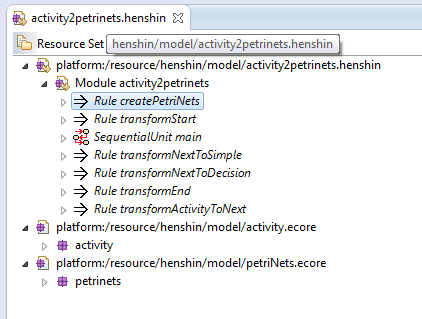
\includegraphics[scale=0.7]{figures/Henshin_TreeEdtiro.png}
	\rule{35em}{0.5pt}
	\caption[The Henshin Model Editor]
	{Tree Based Editor for rules in Henshin.}
	\label{fig:Henshin_TreeEditor}
\end{figure}

\subsubsection*{Defining Meta-models}

The Henshin language requires a source and a target meta-model to be able to
perform model transformations. The target meta-model can either be the same as
the source meta-model or defined in another modeling language. Either way, before
the users can start creating transformation rules, the meta-models has
to be defined. To define these meta-models, Henshin utilizes Ecore, that is
provided by the Eclipse Modeling Framework\cite{Steinberg2009}. Ecore models
can either be created using a tree based editor, called Sample Ecore Model
Editor or by using a graphical editor. While the graphical editor is optional,
the tree based editor is mandatory for creating Ecore models, since this
represents the Ecore model.

Initially the user has to create an EPackage element in the newly created Ecore
model. Henshin interpret instances of this EPackage as EObjects and is what
Henshin searches for when the user want to import an Ecore model. This EPackage
element can have several child elements, like for example EClass, EEnum and
EData type. For this specific example we only needed the EClass element to
create the nodes for the meta-models. For each EClass element the users can
specify an EReference that connects two EClass elements. This means that an
EReference element defines relations between the nodes for the meta-models. To
give an EClass element properties, the user can create an EAttribute element.
This element can be typed, either by a predefined list of types or by defining
user created EData types. For the purpose of this case study we only needed to
name the different nodes and therefore we only needed the data type EString.
Through the use of these Ecore elements, we can create the two meta-models from
figure~\ref{fig:activity_metamodel} and figure~\ref{fig:petrinet_metamodel} that
was previously presented in this chapter. 


\subsubsection*{Defining Transformation Rules}

Now we have defined the source and target meta-model, and imported
both of the meta-models EPackages. We can now use elements from the two
meta-models to create transformation rules in the Henshin transformation
language. In Henshin, objects are referred to as nodes and links between objects
as edges. From the meta-models these nodes represents the EClass elements and
edges is a EReference between these EClass elements. A collection of these
nodes and edges defines a graph structure. Each transformation rule in Henshin
specifies two graphs that represent the LHS and the RHS. Note that the
graphical editor provides an integrated view to creating transformation. And
therefore Henshin handles assignment of modeling elements to the LHS and the
RHS through the use of stereotypes. Figure~\ref{fig:HenshinScreen} represents a
visualization of the graphical syntax and includes a transformation rule,
``transformSimpleActivity''. On the right side there is a palette that contains
Henshin modeling elements and different EPackages. The first two EPackages
represents modeling elements for the source and target meta-model. The Henshin
Trace Model provides support for including traceable links for exogenous model
transformations in Henshin. The Henshin Trace model provides a traceable link
that keeps track of the translated elements during a transformation. This model
consist of a single class Trace, that has two references called source and
target. These references are of type EObject and therefore can refer to any EMF
object. The Trace model is generic and therefore supports creation of traceable
links between any Ecore models.

\begin{figure}[H]
	\centering
	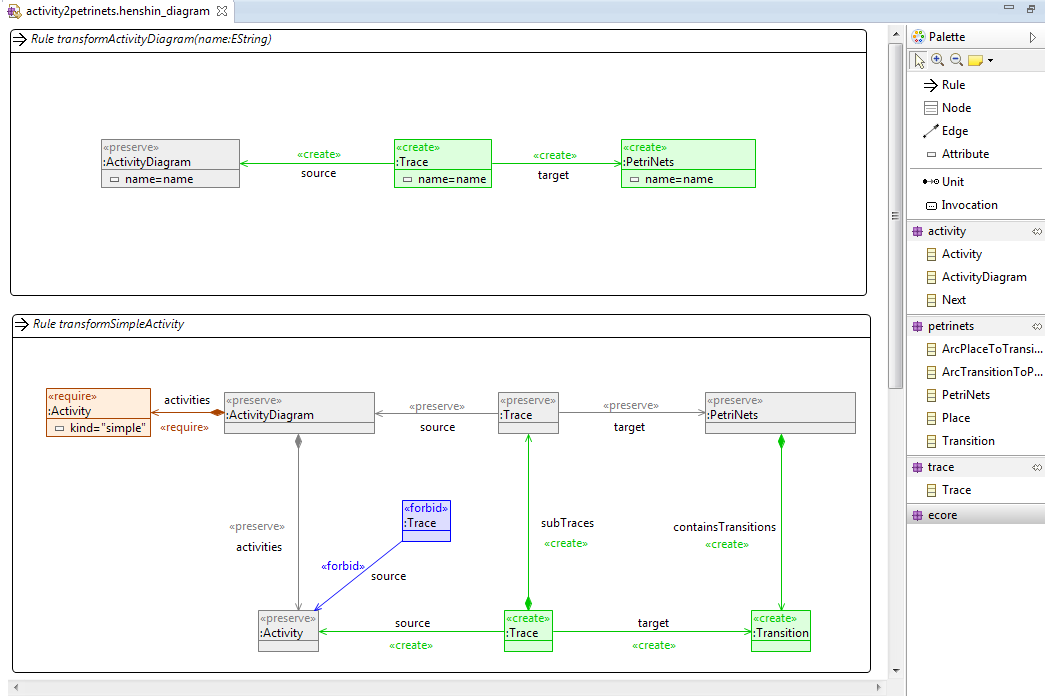
\includegraphics[scale=0.6]{figures/henshin_scren_2}
	\rule{35em}{0.5pt}
	\caption[The Henshin graphical editor]
	{A rules represented in the Henshin graphical editor.}
	\label{fig:HenshinScreen}
\end{figure}


The Node, Edge and Attribute modeling elements are used to define the different
transformation rules in Henshin. A new transformation rule in Henshin always
have to start with creation of a new Rule element. Inside this Rule element the
users are free to create nodes, and connect these nodes with edges. The nodes
and edges defines a graph structure that is used to either locate matches in a
source model or translate target modeling elements. Henshin makes sure that
these nodes and edges conforms to their corresponding meta-models. Note that the
Node and Edge modeling elements are special for Henshin and are used to create
the content of the transformation rules. The Node element has a type that
correspond to an EClass while the Edge element has a type that correspond to an
EReference. Note that the Ecore models that are represented in
figure~\ref{fig:HenshinScreen} has a list of modeling elements that are typed by
EClass. These modeling elements are a shortcut for Henshin to create nodes and
creates a Henshin node with the corresponding type. The Attribute element can be
used if attributes are defined for the classes that are imported. We will come
back to the Unit element in the next section. Henshin distinguish if nodes,
edges or attributes are part of the LHS and the RHS through the use of
predefined stereotypes, or action types. Based on these action types Henshin
automatically specifies if these modeling elements defines a graph structure
that is used to locate matches in a source model or produce modeling elements
for a target model. If the action type consist of the sequence ``create'',
Henshin knows that this element should be part of the replacement graph, or the
RHS. While on the other side, the sequence ``delete'' should be part of the
pattern graph, or the LHS. The ``preserve'' sequence is a bit more special,
because nodes or edges in Henshin that is specified by this action type should
be part of both the LHS graph and the RHS graph. This is done by putting the
preserve element in both graphs and then create a mapping between these two
elements to inform the Henshin Interpreter that this represents the same
element. Henshin also has support for application conditions. The action types
``forbid'' and ``require'' are used for defining Negative Application
Conditions (NACs) and Positive Application Conditions (PACs). These actions are
supported for nodes, edges and attributes. The example rule in
figure~\ref{fig:HenshinScreen} use four of these action types. The modeling
elements in gray represents modeling elements that are part of both the RHS and
the LHS graph, while the modeling elements in green are specified in the RHS
graph. This specific transformation rule will locate a matching pattern in a
source model that is described by an Activity modeling element. The positive
application condition specifies that Henshin only should locate matches that is
of kind ``simple''. The negative application condition specifies that a
located match that is described by the Activity class should not have a
traceable link. The NAC specifies that the transformation engine does not locate
duplicate matching patterns. The first time a match is located a traceable link
is established. Now this specific match is no more a valid match since the NAC
forbids the transformation engine to locate matches that already has established
a traceable link to this modeling element. Note that we have a Trace and a
PetriNets that is both a preserve modeling element. This is because these two
are already translated by another transformation rule.

\subsubsection*{Application Control for the Transformation Rules}
Transformation units are used to administrate the different transformation
rules. Henshin provides several different units with different properties.
Note that a transformation rule is also a transformation unit. This means that
it is unnecessary to create a unit in Henshin if our model transformation only
consist of one transformation rule. But if there are more than one 
transformation rule there has to be a control mechanism that determines how
these transformation rules should be applied. An Independent Unit is applies
rules non-deterministically and is a good solution if the order of applying the
transformation rules is not important. But if the transformation rules requires
a very strict pattern and are dependent of other rules, then a sequential unit
are a safe way to apply rules. The sequential unit forces the Henshin
transformation engine to apply rules in a sequenital order.
Figure~\ref{fig:SequentialUnitHenshin} is an example of a sequential unit
that will start applying rules at the black circle and follow the arrow
through each given rule until it is finished.  

\begin{figure}[H]
	\centering
	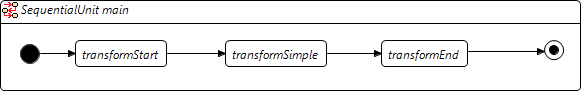
\includegraphics[scale=0.7]{figures/SequentialUnitHenshin_1.png}
	\rule{35em}{0.5pt}
	\caption[A Sequential Unit in Henshin]
	{A SequentialUnit main that contains a sequence of rules.}
	\label{fig:SequentialUnitHenshin}
\end{figure}

If applicable a transformation unit can also consist of other units, for example
if the user want to either iterate or loop through a transformation rules. The
previous section described an example of a rule in
figure~\ref{fig:HenshinScreen}. The sequential unit above the
``transformSimple'' represents a LoopUnit while the ``transformStart'' and
``transformEnd'' represents a single rule. The loop unit applies a single
transformation rule until there are no more matches found in a source model.
This is convenient for the rule, ``transformSimpleActivity'' since we specified
that the rule should only locate matches where there exist no traceable link.
Henshin also has two other units that can administrate transformation rules,
namely ConditionalUnit and PriorityUnit. The ConditionalUnit follows a if-else
pattern, and is used if the user want Henshin to choose between other units.

\subsubsection*{Translating the instance model}

Now that we have defined the source and target meta-model, created a set of
transformation rules and initialized a control mechanism for these rules it is
time to apply the transformation rules. For Henshin there is two ways to do
this. In Henshin the default engine for executing model transformation is the
Henshin interpreter. This interpreter can be invoked either by using the a
Eclipse wizard or programmatically using the Henshin API. 

Using the Eclipse wizard is done by opening the Henshin file in the Henshin
Model Editor and right clicking the root object and locate apply transformation.
This will open a wizard where the user can choose a transformation unit. This
will either be a single transformation rule or some transformation unit that
applies all other units and rules. The user also has to select the instance
model and can explicitly set parameters for the rules if this is applicable. If
the parameter is set to Ignore then the interpreter will automatically match the
parameter. Now the user has two choices, the first choice is to preview the
result of the model transformation. This will either show the user a new window
with the modifications to the model or a message that the rule or unit could not
be applied. If the user press Transform instead of Preview, the model will be
transformed and saved.

The interpreter can also be invoked programmatically, either as an
Eclipse based application or as a simple Java application. Henshin provides a
API that lets the users invoke the interpreter through the use of Java code.
There is a class HenshinResourceSet that lets the user load and save models and
transformations. When the instance model and Henshin module is loaded into the
resource set, the transformation can be applied through the use of the Henshin
Engine class. This is where Henshin finds and translates matches found in the
instance graph. The user also has to specify the main transformation unit from
the Henshin module. Both the engine and the unit can be loaded into the
UnitApplication class. And this class has a method called execute that lets the
user execute the model transformation. If the transformation was executed
without errors, then the instance model can be saved with the translated
changes. The Henshin API lets other users use the power of Henshin in their own
program.

\subsection{ATL Transformation Language}

ATL\cite{ATL} (ATL Transformation Language) is a model transformation
language and is an implementation of the QVT\cite{QVT} standard. It
provides ways to produce a set of target models from a set of source models.
ATL is maintained by OBEO\cite{OBEO} and AtlanMod\cite{ATLANMod} and was first
initiated by the AtlanMod team, previously called the ATLAS Group, located at
the University of Nantes in France. The initial version of ATL was created In
2004, where ATL became part of the Eclipse Generative Modeling Technologies
(GMT) \cite{GMT}. The goal of GMT is to produce a set of research tools in the
area of Model Driven Software Development. The ATL Integrated Development
Environment (IDE) was later promoted for the Eclipse M2M project in January
2007.

There are developed several tools that has support for a declarative
approach to model transformation. For the purpose of this paper, we will explain
this approach with the focus around the Atlas Transformation Language (ATL).
ATL is a hybrid model transformation approach, that is a transformation
language that combines other model to model transformation approaches. For
example, ATL provides transformation rules that can be either fully declarative
or fully imperative or a mixture of both. 

\begin{figure}[H]
	\centering
	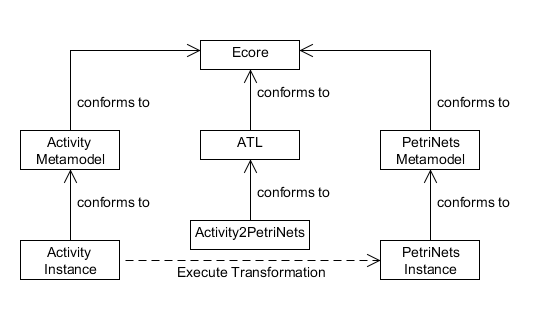
\includegraphics[scale=0.55]{figures/ATL.png}
	\rule{35em}{0.5pt}
	\caption[Model transformation for Atlas transformation language]
	{Model transformation process for Activity2PetriNets.}
	\label{fig:ATL}
\end{figure}

Figure~\ref{fig:ATL} gives us an idea of how the ATL transformation from an activity
diagram to Petri net are handled. We want to generate a instance of PetriNets,
that conforms to its own meta-model. This is generated from a source
model, Activity Instance, that conforms to its respective meta-model.
The created transformation Activity2PetriNets is expressed in the ATL
transformation  language, that conforms to its own meta-model. These three
meta-models conform to the meta-model Ecore. So this makes Ecore a metameta-model
to represent the meta-models of Activity, ATL and PetriNets.

ATL has to be configured properly before the user can execute a model
transformation. In this configuration both the location of the source and target
meta-model has to be specified. The user also has to specify what instance model
that should be translated. And lastly the user has to create a new file that can
be specified as the target instance model for the ATL run configuration. The
user can then initiate the transformation by running this as an ATL
transformation.


\subsubsection*{Textual editor}

ATL can be compared to a programming language, because it is
basically a transformation language that provides a concrete textual syntax. ATL
is a text based transformation language, and is build around the Object
Constraint Language (OCL) \cite{OCL} with some additional predefined functions.
ATL transformations is stored in a file extension called ``.atl'' These ATL
files can contain different kind of ATL units and are defined in its own
distinct ATL file. These different ATL units are ATL modules, ATL queries and
ATL libraries. Libraries can be used to create independent ATL libraries that
can be imported to different types of ATL units. The module unit specifies the
different application rules for a  model transformation. And the Queries are
used when the users want to compute primitive values from the source models.

Now that we have specified these three ATL units, we can describe shortly how
we can use the ATL transformation language to create model to model
transformations. For our case study, we only need the ATL modules. An ATL module
corresponds to a model to model transformation. This unit enables developers to
specify the way to produce a set of target models from a set of source models.
The source and target models of an ATL module must be consistent with their
respective meta-models. 

\subsubsection*{Defining Meta-models}

Defining meta-models for the ATL language is defined by the modeling language
Ecore. Since defining the meta-models are defined similar as Henshin, see
chapter 4.2 for more details. 

At first, the user start out with a blank ATL file. Since we are working in
the ATL Integrated Development Environment for Eclipse, we want to start the
document with defining the path to the source and the target meta-model. The
reason for doing this is to achieve auto completion from elements defined in the
Ecore meta-models. This is convenient for the users when creating transformation
rules.  

\begin{figure}[H]
	\centering
	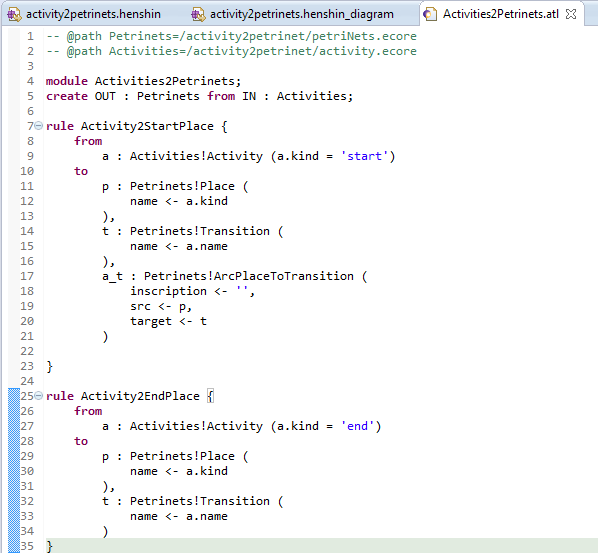
\includegraphics[scale=0.5]{figures/ATLScreen.png}
	\caption[Simple rules for ATL]
	{Two simple rules for Activity2PetriNets in ATL.}
	\label{fig:ATL_Screen}
\end{figure}

Next the file is composed of four different elements. The first element is the
header section, where the user can give the module a name and name the variables
corresponding from the source and target models. The module name has to be
identical to the name of the ATL file.

We also need to specify the source and the target meta-model. From
figure~\ref{fig:ATL_Screen} we can see that the target meta-model is initialised 
with the keyword create, and the source meta-model is initialised using the
keyword from. The user can also import some existing libraries if needed. This
import section is however optional. Importing meta-models are handled a bit
differently in ATL compared to Henshin. In ATL the meta-models are imported
explicitly while in Henhsin they are imported implicitly before they can be used
in modifying the transformation rules. For ATL the user has to configure where
both the source and the target meta-model are located through a configuration
page. 

The next element is a set of rules that defines how the target models are
generated from the source models. These rules are used to implicitly match
source elements and produce target elements. In figure~\ref{fig:ATL_Screen} we
have examples of two rules, namely the rule for transforming the start activity
and the rule for transforming the end activity. We can see that for each rule we
specify what we want to translate from and what we want to translate to. We will
describe transformation rules in more details in the next section.

The last element in a ATL module is a set of helper functions. This collection
of helpers can be compared to Java methods. These helper methods can be used to
make the transformation rules easier to read for example.

\subsubsection*{Transformation Rules}

A rule in ATL describes how a target model should be generated from a source
model. In ATL there are three kinds of rules, the type matched rules and the
lazy rules are both fully declarative while the called rules are imperative.
These rules has an input pattern and an output pattern. The input pattern can
have a list of source model elements that is part of a rule in ATL by defining
several input pattern elements. Each input pattern element has to have a
mandatory type that corresponds to a metaclass defined in some meta-model. Each
rule corresponding input pattern can also specify optional conditions that are
expressed as OCL expressions. Both the type and an optional condition specifies
which elements from the source model that is matched for each rule. The output
pattern defines how the target model elements are created from the input model. 

\textbf{The matched rules} provides an declarative approach to
creating transformation rules in ATL. The users can specify from which kinds of
source elements the target elements can be generated from and how the generated
target elements should be initialized. A matched rule finds a match according to
the type of source model element and generate target model elements from these
matches. A new matched rule is defined by the keyword ``rule'' and has two
mandatory and two optional sections. The mandatory sections specifies the input
pattern and the output pattern while in the first optional section the users can
declare and initialize local variables. Note that these variables can only be
used in the scope of each rule. The second optional section includes an
imperative section The type that is introduced in the input pattern conforms to
a meta-element in a meta-model of the source model. This rule will then generate
target elements according to each match in the source model.

Figure~\ref{fig:ATL_Example} shows a simple rule, Activity2StartPlace that wants
to translate Activity source elements to some target elements. This rule
specifies the keyword \textit{from} for the input pattern and \textit{to} for
the output pattern. For this example we want to find matches for one source
element that is of type Activity that conforms to the meta-model Activities. We
also provide additional properties for this input source element, where we only
want to find matches that conforms to the type Activity and has the name
``start''. The rule specifies that we want to generate three target
pattern elements p, t and a\textunderscore t from this matching type. These
generated target elements conforms to the meta-model Petrinets and specifies
that these generated types should generate attributes from the source
pattern element. The generated target model elements is initialized with
attributes from the matched source pattern element. 

\begin{figure}[H]
	\centering
	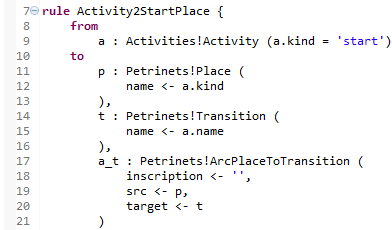
\includegraphics[scale=0.7]{figures/ATL_Example.png}
	\caption[Example of a matched rule in ATL]
	{An example of a matched rule in ATL.}
	\label{fig:ATL_Example}
\end{figure}

If applicable the users can add an optional condition for each rule to check for
certain matches for this input element. This condition is expressed as an OCL
expression and gives the user the possibility to restrict the searches of the
source elements. 

The second type ATL rules are \textbf{Lazy rules}. These lazy rules will
never be applied when a model transformation in the Atlas Transformation
Language is executed. These lazy rules can only be applied to a model
transformation when they are called from another of the two rules. These lazy
rules are created similar to the matched rules.

The third and final type for an ATL rule is called \textbf{Called rules}. A
called rule has to be called from an imperative section from either a match rule or
from another called rule. A called rule is created similar to a matched rule,
namely with a \textit{rule} keyword. One thing that is special with a called
rule is that it does not have to match source elements from the source model.

\subsubsection*{Execution of an ATL transformation}

Figure~\ref{fig:ATL_Execution} describes the architecture of the transformation
language. From the figure we can see that we have an association between EMF and
Ecore models. This are the meta-models that are expressed using EMF's Ecore
model. These meta-models are then translated through a model handler that
compiles these Ecore models to the ATL Virtual Machine. Where these meta-models
can be used both in creating ATL programs and in ATL's internal interpreter. The
ATL compiler translates the ATL file into a new ASM assembler file, that ATL can
use to launch a model transformation. This assembler file contains the
compiled code of the corresponding ATL file.

\begin{figure}[H]
	\centering
	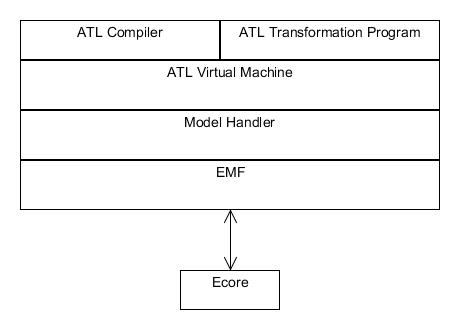
\includegraphics[scale=0.6]{figures/ATL_Execution.png}
	\caption[Internal infrastructure for ATL]
	{Internal infrastructure of for ATL.}
	\label{fig:ATL_Execution}
\end{figure}

The default semantics for executing a set of transformation rules specified in
ATL can be described in three phases. See ATL User Manual\cite{ATL_USERMAN} for
more information.

The first phase is an initialization phase. This phase consist of amongst other
things to initialize the trace model and the module of the ATL transformation.
The trace model in ATL has one important function, and that is to create a
trace link that points to the matched source input elements and the
corresponding generated target output elements. The trace model in ATL works as
an implicit tracing mechanism that specifies relationships between the source
element and its corresponding target elements by using a native type called
ASMTransientLink\cite{Wagelaar}. For every time a transformation rule is
matched to a source element, one ASMTransientLink is created. To this transient
link the name of the transformation rule provided together with the source
element and the target elements. These links are added to a collection that is
stored internally for ATL. This means that the users of ATL cannot access these
links after a model transformation has finished executing. However, as shown by
Andr\'{e}s Yie and Dennis Wagelaar\cite{Wagelaar}, that gaining access to these
ATL traces can be done explicitly by creating transformation rules that
generates a tracing model based on the internal tracing information provided by ATL.

The next phase consist of finding matches in the source pattern of the matched
rules. This is done by the ATL transformation engine that searches for valid
matches. A match is valid when all input pattern elements are found amongst
the source model elements and any OCL expression for that matched rule is valid.
The transformation engine also allocates the target model elements based on the
declared output pattern into memory. At this point the target model elements are
only allocated, they are initialized in the final phase. For each match found,
there is created a trace link that has a source link to the matched source
elements and a target link to the generated target elements. The generated
target elements are not given any attributes or properties in this phase. This
phase create target elements from matches found, and create a trace link between
them.

The final phase of for executing an ATL module is to initialize the target model
elements. At this stage each allocated target model element are given
attributes and features that corresponds to the matched rule. The ATL
transformation engine now use the trace links to determine the matched source
elements and the generated target elements. This operation is called
resolveTemp, that returns the reference from the target model elements that
where generated in the second phase and to the corresponding source model
element. Now that these three phases is finished the ATL transformation engine
can execute the imperative code sections defined for the module. 

\section{Model transformation environment for DPF}
\label{tool_choice}

After working with the three model transformation environments in the previous
section we decided to try and integrate Henshin with DPF. In this section we
will describe why Henshin is the better choice of the three considered
environments to integrate with DPF. Henshin\cite{Henshin_2010,Henshin} is a
relatively new installment in the world of model transformations. The
environment was initially created three years ago, in 2010 and is marked as an
Eclipse Incubation project. The purpose of the incubation phase is to establish
a fully functioning open-source project. In theory an integration of Henshin
with the DPF should be possible, since Henshin applies model transformations
based on Ecore models and DPF models are basically represented as Ecore
models. This presents a problem with integrating AGG with DPF. In EMF the root
of all modeling objects is an EObject that has no references to a Java Object. 
AGG could also be integrated with DPF, but the problem is that this would
require an extensive amount of manual coding. We could use AGG as a general
purpose graph transformation engine in a java applications. We would have to
create the source model as an AGG graph and a type graph based on the source and
target modeling formalism that DPF provides. AGG provides an API that
conveniently let us create type graphs, source graphs, transformation rules and
application conditions.
 
\begin{figure}[H]
	\centering
	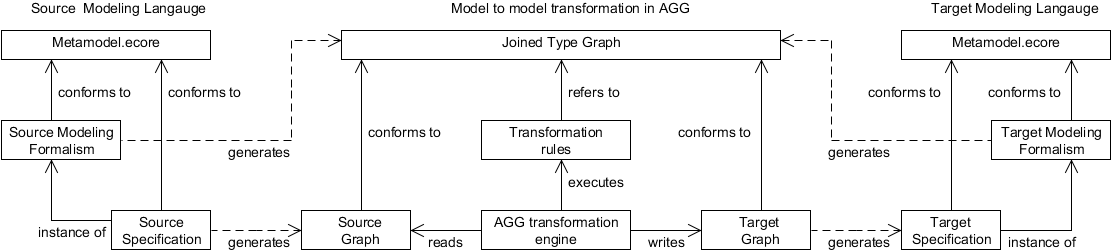
\includegraphics[scale=0.52]{figures/AGG_solution.png}
	\caption[Proposed solution for integration of AGG]
	{Proposed solution for integration of AGG with the DPF Workbench.}
	\label{fig:AGG_Solution}
\end{figure}

Figure~\ref{fig:AGG_Solution} represents a proposed solution how to integrate
AGG together with a DPF transformation tool. The figure represents a source
modeling formalism on the left side, a target modeling formalism on the right
side and a model to model transformation done with AGG in the middle. The
figure informs us that we have to generate four models to be able to do this in
AGG. First we create the abstract syntax for an AGG source graphs by generating
a joined type graph from a source modeling formalism and target modeling
formalism. Then we have to generate the source input specification into a source
graph that at the same time conforms to the joined type graph. Note that we do
not mention the transformation rules since we have to generate these regardless
of what model transformation environment we integrate with the DPF workbench.
After the AGG transformation engine have executed the transformation rules we
have to generate a target specification based on the produced target graph. This
leads to some potential problems. The program that generates a source graph and
a target specification has to be solid and not contain any flaws. Another
problem is to keep the models consistent throughout the model transformation.
How can we be certain that the target graph is consistent with the target
specification? It is easy to loose consistency when changing a model manually
from a target graph to a target specification. We could use AGG to do this, but
that leads to many potentially factors that could go wrong. With Henshin and
ATL we are not required to do anything extra with these models. Since both
environments has support for including Ecore models as meta-models and requires
an instance model of an Ecore model as a source model to apply a model
transformation. Therefore AGG can be integrated with EMF with some additional
work, but Henshin and ATL is a more viable choice for DPF, since we can use
this Metamodel.ecore as a meta-model and the source specification as input
model directly in the other two environments. 

Now we need to decide if we want to try and integrate the hybrid model
transformation environment, ATL or the graph based model transformation
environment, Henshin. In section~\ref{sec:DPF} we discussed that a DPF model is
an extension of the Generalised Sketches formalism which is basically a directed
graph. Then a specification consist of a set of nodes, edges and two functions
that preserve a source and a target node for all edges. A model transformation
in Henshin is based on the concepts of graph transformations and category
theory. We can then be certain that Henshin can interpret a source specification
as a directed graph. Henshin transformation is also based on the two graph
transformation styles single (SPO) and double pushout (DPO) that we discussed in
section~\ref{sec:graph_based}. And we recall that the DPO approach provides a
dangling condition that ensures that a model transformation does not result in
any edges that are missing a source or a target node. We want to create a tool
for the DPF workbench that provides the following. 

\begin{itemize}

\item \textit{Concrete Graphical Syntax}. We want to be able to create
transformation rules based on graphical syntax that the DPF Editor provides.

\item \textit{Generic}. We want our tool to work for an arbitrary source and
target meta-model regardless of abstraction layer. 

\end{itemize}

The tool is required to create a set of transformation rules based on some
model transformation language and we want these transformation rules to be
generic. This means that we create a set of transformation rules based on an
arbitrary source and target meta-model. The only aspect of these meta-models
that is consistent is that they contain a list of nodes and arrows. This means
that regardless of abstraction layer a specification is specified by a set of
nodes and arrows. The reason for why we decided to try and integrate Henshin
within the DPF workbench is provided in the three items underneath. 

\begin{enumerate}

\item We want to create a tool that use a simplified version of the DPF Editor
to create transformation rules that provides a concrete graphical syntax. DPF
models are already based on category theory and provides a graphical syntax. 

\item Through the use of the Henshin meta-model we can generate a set of
transformation rules that are based on the abstract syntax of the source and
target specification. We can define a set of transformation rules in Henshin
as a java application with the help of the API that Henshin provides. 

\item We can utilize the concepts around graph transformation that provides a
left hand side, a right hand side and an intersection graph. Through these three
graphs we can in Henshin use the single or double pushout approach when applying
a set of transformation rules. 

\end{enumerate}

The problem with integrating Henshin with DPF is that Henshin is based on the
EMF technology, and therefore utilize OMG's MOF. Henshin supports out of the
box model transformation that translate instance models that conforms to an
Ecore based meta-model. These instance models provides the concrete syntax of a
modeling language and are described by a corresponding meta-model that
represents the abstract syntax. This meta-model is provided accordingly to the
second layer of the Meta-Object Facility. This means that Henshin provides model
transformation according to EMF's two layered modeling environment. DPF on the
other hand provides initialisation of a potential endless hierarchy of
meta-modeling, and therefore does not match the steps MOF provides to create
the abstract syntax for a Domain Specific Language. We know that a
transformation rule in Henshin requires references to meta-modeling elements
from a source meta-model and a target meta-model. What makes a DPF
specification special is that it is an instance model of both an Ecore based
meta-model and another specification. This means that a specifications concrete
syntax is typed by the abstract syntax of a specification that is one
abstraction layer higher. In DPF we can create an arbitrary level of
meta-models and therefore two different Domain Specific Modeling Language can
be defined over a different abstraction layer hierarchy. The Henshin
environment has strict guidelines on how models are imported and used. These
models are required to be created accordingly to the Ecore model provided by
EMF. Henshin can then utilize these models to create a graph pattern that
structure both the LHS and the RHS graph of a transformation rule. Now the LHS
graph contains a graph structure that is is used by the transformation engine
to locate matches in an instance model that conforms to the specified Ecore
model.

For our tool we can structure a set of transformation rules in Henshin based on 
this common meta-model, \textit{Metamodel.ecore} that all specifications
$\spec{S}$\textsubscript{1\ldots n} conforms to. We have to threat all
specifications similar if we want the tool to provide a generic model to model
transformation. The challenge with integrating Henshin in a language workbench
that provides meta-modeling at arbitrary layers of abstraction is not in the
source specification we want to translate, but in the instance specification
that the source specification corresponds to. This proves to be a problem for
Henshin, because we cannot import an instance model of an Ecore based meta-model
into the Henshin model transformation environment. We can do changes to an
instance model by using Henshin, but the transformation language can only
import and utilize models that conforms to the Ecore meta-model. To solve this
for DPF specifications we expand transformation rules in Henshin with
application conditions. This means that we restrict the LHS graph to locate
matching modeling elements in an instance source specification based on the
abstract syntax that another specification provides. The next chapter provides
an explanation on how we integrated Henshin for a transformation tool that
provides model to model transformations for the DPF workbench.





%----------------------------------------------------------------------------------------
%	SECTION 2
%----------------------------------------------------------------------------------------

 
%% Chapter Template

\chapter{Related Work} % Main chapter title

\label{Chapter5} % Change X to a consecutive number; for referencing this chapter elsewhere, use \ref{ChapterX}

\lhead{Chapter 5. \emph{Related Work}} % Change X to a consecutive
% number; this is for the header on each page - perhaps a shortened title

\section{The Attributed Graph Grammar System}

AGG is a general development environment for algebraic graph
transformation systems. AGG is provided with a graphical editor for creating
and modifying graphs. The editor provides a graphical user-interface with
several visual editors for applying the principles of graph transformation. It
also has an interpreter and a set of validation tools. AGG is ongoing research
activity of the graph grammar group at TU Berlin. The work on AGG started in 1997.

\subsection{Graphical Editor}
The graphical editor of AGG, represented in
figure~\ref{fig:AGGScreen}, has several functions to help the user to define
model transformations. In the top left corner of the graphical user-interface
is a tree based editor for defining rules and grammar. This tree based editor
also contains the type graphs and the host graphs. Where the host graph
represents some input model for a model transformation.

Each application rule has two visual editors, representing the left
(LHS) and the right hand side (RHS), or the pattern and the replacement graph.
In the tree based editor containing rules and grammars it is possible to give
rules application conditions. This is convenient if the user wants to have
constrains for the pattern or the replacement graph.

In the tree based visual editor it is also possible to define host
graphs and type graphs. Type graphs is described more in depths in the next
section, but roughly said, the type graph defines elements that can be used in
the host graph. Type graphs defines the abstract models for the host graph and
is similar to how Ecore defines metamodels  for EMF and the Meta Object
Facility (MOF)\cite{MOF}, that is a language for defining abstract syntax of
modeling languages. The users can now create instances from these type graphs.
These instances represents the host graphs and corresponds to its concurrent
type graph.

For the application rules, the user can extend the attributes with Java
expressions. This means that the users can use Java primitives such as strings,
integers or float numbers to form the pattern graph or the left hand side of
the rule. The user cannot bind attributes that is not initialised in the type graph.

In figure~\ref{fig:AGGScreen} there are some node elements and association
elements to the right side of the figure. These are meta elements that are
initialized in the type graph. These meta elements are used to create the host
graph, the different transformation rules and application conditions. The host
graph is not consistent with the type graph, since these meta elements are
initialized in the type graph. Its worth mentioning that both the
node elements and association elements in the figure has been scaled up for the
purpose of this paper.

\begin{figure}[H]
	\centering
	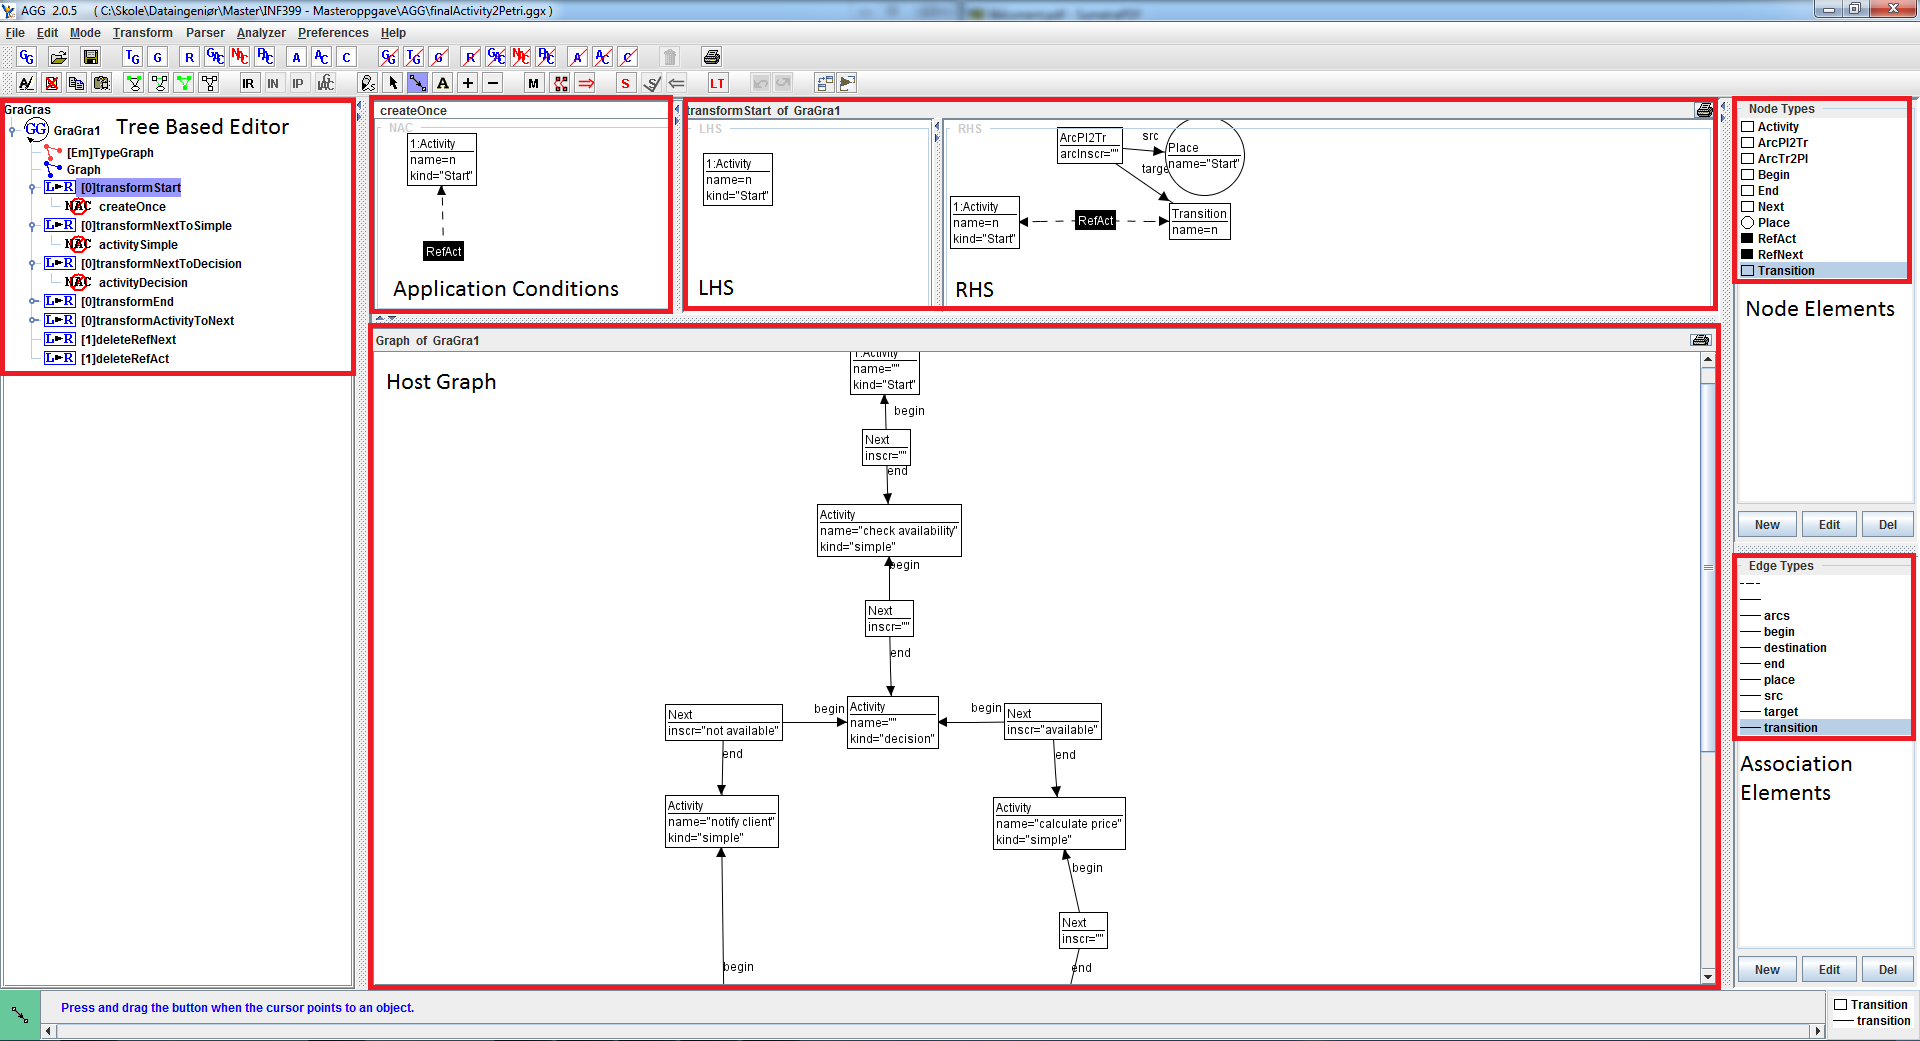
\includegraphics[scale=0.3]{figures/AGGscreen.png}
	\caption[Graphical Editor for AGG]
	{A model transformation for the AGG Editor.}
	\label{fig:AGGScreen}
\end{figure}

\subsection{Defining Metamodels}

Before the host graphs can be created, we have to initialise the AGG
tool with the metamodels. In AGG both the source and the target metamodel are
defined in a common type graph. This type graph represents the abstract syntax
for the host graph. If we want to prepare an AGG graph for a transformation, we
create a single type graph with references between elements of both source and
target metamodel. This way, when the application rules is executed, we can
choose to keep both the source graph and the references between these elements.
The references and source graph can be deleted through a cycle of transformation rules.

\begin{figure}[H]
	\centering
	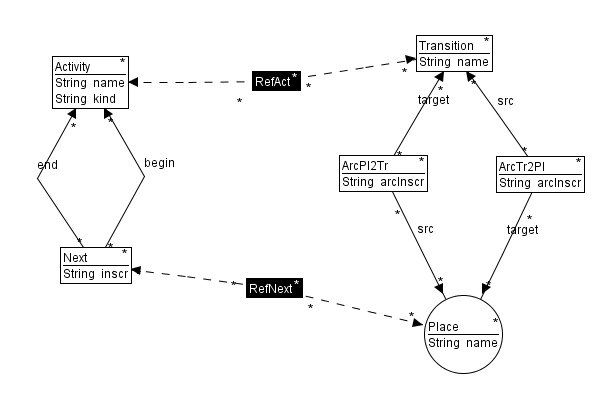
\includegraphics[scale=0.7]{figures/AggTypeGraph.png}
	\caption[Type graph in AGG]
	{Type graph for activity diagram and Petri net in AGG.}
	\label{fig:AggTypeGraph}
\end{figure}

For the type graph, the user must define nodes and arrows for each meta
element for both the source and target model. These nodes and arrows can also
have attributes. Nodes represents elements from the two modelling languages and
arrows represents the associations between these elements. In the type graph we
want to distinguish between associations and references, and therefore we
represent references as a dashed edge. These dashed edges are not given any
attributes, and that is because we want these edges to represent what the
targeted element was translated from. From figure~\ref{fig:AggTypeGraph} we can
see that a RefAct node is defined and is connected between the activity
element and the transition element. The same initialisation is defined between
the next element and the place element. For AGG type graphs there is a
multiplier condition for the edges. This means that there can be an arbitrary,
or a zero to many number of instances of these relations in the host graph.

\subsection{Defining Transformation Rules}
Now the type graph has been initialised and the instance graph of the
source model has been created. But to be able to translate to a target model,
we need to create a set of transformation rules. A transformation rule
require an unique name and a LHS graph and a RHS graph. 

\begin{figure}[H]
	\centering
	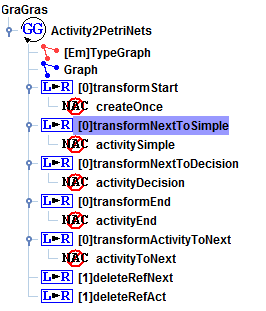
\includegraphics[scale=0.7]{figures/AGGTreeBasedEditor.png}
	\caption[Tree based editor in AGG]
	{Tree based editor for transformation rules.}
	\label{fig:AGGTreeBasedEditor}
\end{figure}

Whenever changes are made in the two graphs, AGG checks if the LHS or the RHS
conforms to the type graph. The user is unable to insert elements in the two
graphs that are not initialised in the type graph and the users are not allowed
by AGG to create associations between nodes that are not initialised in the type
graph. This is how AGG keep the source and target model consistent. In
figure~\ref{fig:AGGTreeBasedEditor} we can see the tree based editor in AGG,
that provides the type graph, the host graph and a list of application rules.
When a new application rule is created, both the LHS and the RHS of this new
rule is initialised. The users can then insert elements in both the LHS and the
RHS depending on how the source model should be translated. 

\begin{figure}[H]
	\centering
	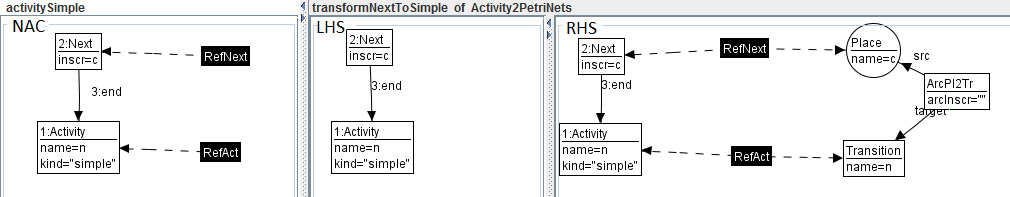
\includegraphics[scale=0.5]{figures/LHSvsRHSAGG.png}
	\caption[Representation of a rule in AGG]
	{The LHS and RHS of a rule and a NAC attached.}
	\label{fig:LHSvsRHSAGG}
\end{figure}

Figure~\ref{fig:LHSvsRHSAGG} is a representation of the rule
transformNextToSimple, with both the LHS and the RHS. Each rule can also
contain application conditions. These can either be Positive Application
Conditions (PAC) or Negative Application Conditions (NAC).
Figure~\ref{fig:LHSvsRHSAGG} has a NAC, activitySimple that makes sure that the
LHS of the rule is translated only once for each pattern match found in the
host graph. Through the use of these application conditions, the users can
create restrictions to how each transformation rule should handle pattern match
in the host graph. Each transformation rule can have multiple application
conditions attached.

\subsection{Administrating Transformation Rules}

By default, the control mechanism for administrating the transformation rules
are set to deterministically. This means that the transformation rules are
executed at random. This option is quite useful if the set of transformation
rules are independent of each other. AGG also provides other ways of applying
rules. These are transformation by applying rule layer or by sequences. When the
transformation is set to be applied by rule layers, then the user can add a
number to the different rules. This layer number will range from 0 \ldots n,
where the lowest number is the first layer and therefore the has first
priority. If there are many rules with the same layer number, then these rules
will be internally transformed deterministically. If the rules are applied
by sequence then the rules will be applied from the first element in the tree
based editor and applying the rest of the rules in sequence.

\subsection{Translating the Host Graph}

Now that we have defined the type graph and created the rules it is time to try
and translate the host graph. The preferred option on how the rules should be
applied has also been set. The user can now either press Start Transformation or
do the transformation one step at the time. When the user use the first option
AGG will apply one rule at the time until there is no more matches to be found.
When AGG cannot find any more matches, the host graph is either correctly
translated or there are errors in the rules. 

The user can also execute the transformation step by step. This will give the
user the same result as the first option, but now the user can do one match at
the time for each rule. 

\section{The Henshin Project}

The Henshin project\cite{Henshin} provides a model transformation
language and an editor for defining model transformations for the Eclipse
Modelling Framework \cite{Steinberg2009}. The Henshin project provides a
transformation language that has support for both endogenous and exogenous
model transformations and a provided graphical syntax. With the help of a
graphical editor, it provides the user with an intuitive way of representing
transformation rules. The Henshin Editor is build on the Eclipse Modelling
Framework and is integrated as an Eclipse plugin. The Henshin Editor was first
developed in a student project at Technical University of Berlin in 2010, and
extended in the bachelor thesis \cite{JohannSchmidt} of Johann Schmidt and the
master thesis \cite{AngelineWarning} of Angeline Warning.

\subsection{Graphical Editor}
Henshin model transformation language is a plugin for the Eclipse
Integrated Development Environment\cite{Eclipse}. The Henshin project provides
the users with a graphical editor to create and modify model to model
transformations. 

The users start out with using the Eclipse wizard to create an empty Henshin
document. The Henshin document is based on the commonly known Extensible Markup
Language (XML)\cite{XML}. If applicable a Henshin diagram file can be created
based on the Henshin file. This gives the users an intuitive approach to
creating model transformation rules.

The Henshin transformation file is represented in a tree based editor in
Eclipse called Henshin Model Editor. In this tree based editor it is possible
to include metamodels for both the source and the target model, represented in
figure~\ref{fig:Henshin_TreeEditor}. This figure represents the Henshin
Model Editor, where the different transformation rules for this case study is
presented. From this figure we can see that there is a Module element called
activity2Petrinets. This Module element will always be the root element for a
Henshin model transformation. This Module element contains all the user created
rules for performing a model transformation in Henshin. There is also two
external Ecore models included in the editor, more specifically the two
metamodels. These metamodels are created based on the EMF standard for creating
models and are independent of one and another.

\begin{figure}[H]
	\centering
	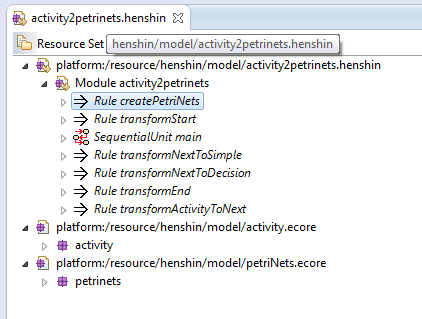
\includegraphics[scale=0.7]{figures/Henshin_TreeEdtiro.png}
	\caption[The Henshin Model Editor]
	{Tree Based Editor for rules in Henshin.}
	\label{fig:Henshin_TreeEditor}
\end{figure}

\subsection{Defining Metamodels}

The Henshin language requires a source and a target metamodel to be able to
perform model transformations. The target metamodel can either be the same as
the source metamodel or defined in another modelling language. Either way, before
the users can start creating transformation rules, the metamodels has
to be defined. To define these metamodels, Henshin use Ecore, that is
provided with the Eclipse Modeling Framework\cite{Steinberg2009}. Ecore models
can either be created using a tree based editor, called Sample Ecore Model
Editor or by using a graphical editor. While the graphical editor is optional,
the tree based editor is mandatory for creating Ecore models, since this is the
actual Ecore model. 

First the user has to create an EPackage element in the newly created Ecore
model. This EPackage is what Henshin searches for when the user want to import
an Ecore model. This EPackage element can have several child elements, like for
example EClass, EEnum and EData type. For our case study we only needed the
EClass element to create the nodes for the metamodels. And for each EClass
element the users can create EReference elements that can be connected with
other EClass elements. This means that an EReference element defines relations
between the nodes for the metamodels. To give an EClass element properties, the
user can create an EAttribute element. This element can be typed, either by a
predefined list of types or by defining user created EData types. For the
purpose of this case study we only needed to name the different nodes and
therefore we only needed the data type EString. Through the use of these Ecore
elements, we can create the two metamodels from
figure~\ref{fig:ActivityMetamodel} and figure~\ref{fig:PetriNetsMetamodel} from
problem specification in the first chapter.


\subsection{Defining Transformation Rules}

Now we have defined the source and target metamodel, and imported
both of the metamodels EPackages into the henshin model. We can now use elements
from the two metamodels to create transformation rules in the henshin model
language. In Henshin, objects are referred to as nodes and links between objects
as edges. From the metamodels these nodes represents the EClass elements and
edges is a EReference between these EClass elements. A collection of these nodes
and edges form a graph. This graph is what represent a transformation rule in
Henshin. It is also possible to define variables for each rule. These variables
can then be used to pass along attributes amongst nodes inside the
graph. 

Each transformation rule in Henshin will have two graph assigned.
These two graphs represent the LHS and the RHS of the rule. One thing that is worth mentioning is
that when working with the graphical editor, these graphs are unavailable for
the users to create or modify. Henshin handles assign the LHS and the RHS
through the use of stereotypes. Each rule can be represented as a graph in the
graphical editor. Figure~\ref{fig:HenshinScreen} is a visualization of the
graphical syntax of a specific transformation rule in Henshin.

\begin{figure}[H]
	\centering
	\includegraphics[scale=0.5]{figures/Henshin_Screen.png}
	\caption[The Henshin graphical editor]
	{A model transformation in the Henshin graphical editor}
	\label{fig:HenshinScreen}
\end{figure}

This rule is responsible for handling the start element for an activity.
On the right side there is a palette that contains Henshin elements and
different EPackages. The first two EPackages contains elements from the
metamodels we created. The next two EPackages are other models that can
be imported into Henshin. The Henshin Trace model is an EMF model that is used
to keep track of the translated elements during the transformation. This model
consist of a single class Trace, that has two references called source and
target. These references are of type EObject and therefore can refer to any EMF
object. This trace object can be used for all imported models used
in Henshin, since these models has to be defined from the Ecore model. Through
the use of the elements in the palette on right side of the window, the users
can create and modify elements. 
The Rule, Node, Edge and Attribute elements are used to define the different
transformation rules in Henshin. A new transformation rule in Henshin always
have to start with creating a new Rule element. Inside this Rule element the
users are free to create nodes, and connect these nodes with edges. At
all time Henshin makes sure that the created nodes and edges conform to their
corresponding models. The Attribute element can be used if attributes are
defined for the classes that are imported. The Unit element we will come back to
in the next section.

Henshin distinguish elements between the LHS and the RHS through the
use of predefined stereotypes, or action types. Henshin automatically delegates
these elements to the RHS or the LHS from these action types. If the action type
consist of the sequence <<create>>, Henshin knows that this element should be
part of the replacement graph, or the RHS. While on the other side, the sequence
<<delete>> should be part of the pattern graph, or the LHS. The <<preserve>>
sequence is a bit more special, because nodes or edges in Henshin that is of
this action type should be part of both the LHS graph and the RHS graph. This is
done by putting the preserve element in both graphs and then create a mapping
between these two elements to inform the Henshin Interpreter that this is the
same element.

Henshin also has support for application conditions. The action types <<forbid>>
and <<require>> are used for defining Negative Application Conditions (NACs)
and Positive Application Conditions (PACs). These actions are supported for
nodes, edges and attributes. Figure~\ref{fig:HenshinAction} is a representation
of how the users can choose amongst these action types.  

\begin{figure}[H]
	\centering
	\includegraphics[scale=0.5]{figures/Henshin_Action.png}
	\caption[Action type for Henshin]
	{Action types for a Node.}
	\label{fig:HenshinAction}
\end{figure}

The ``Multi-node`` is a very special Henshin action type. This Henshin
feature gives the users the possibility to create nested multi-rules. This
concept used to be defined as an amalgamation unit in Henshin, but this feature
was changed to give users the opportunity to create rules inside rules. A
multi-rule action type would then be changed to <<create*>>, where the star
informs Henshin that this is a multi-rule. The Path option gives the users
the opportunity to give name this multi-rule. Multi-rule can be very useful if
there is a pattern in the instance graph that is matched more than once. The
users can then use this nested multi-rule concept to match and apply this rule
as often as possible.

\subsection{Transformation Units}
Transformation units in Henshin are used to administrate the different
transformation rules. There are several different units in Henshin that all have
different properties. It is important to mention that a rule is a unit,
since it inherits from a unit in the Henshin metamodel. This means that it is
unnecessary to create a unit in Henshin if our model transformation only
consist of one transformation rule. But if there are defined several
transformation rules there has to be a control mechanism that determines how
these transformation rules should be applied. A Independent Unit is a good
solution if the order of applying the transformation rules is not important.
But if the transformation rules follows a very strict pattern and are dependent
of other rules, then a sequential unit are a safe way to apply rules. The
sequential unit forces Henshin to apply rules in a given order.
Figure~\ref{fig:SequentialUnitHenshin} is an example of a sequential unit
that will start applying rules at the black circle and follow the arrow
through each given rule until it is finished.  

\begin{figure}[H]
	\centering
	\includegraphics[scale=0.5]{figures/SequentialUnitHenshin.png}
	\caption[A Sequential Unit in Henshin]
	{A SequentialUnit main that contains a sequence of rules.}
	\label{fig:SequentialUnitHenshin}
\end{figure}

If applicable a transformation unit can also consist of other units, for example
if the user want to either iterate or loop through a transformation rules. This
can also be done with the use of a multi-rule, but in some cases this can only
be done by a LoopUnit or a IterateUnit. Henshin also has two other units that
can administrate transformation rules, namely ConditionalUnit and PriorityUnit.
The ConditionalUnit follows a if-else pattern, and is used if the user want
Henshin to choose between other units. 

\subsection{Translating the instance model}

Now that we have defined the source and target metamodel, created a set of
transformation rules and initialized a control mechanism for these rules it is
time to apply this transformation. For Henshin there is two ways to do this. In
Henshin the default engine for executing model transformation is the Henshin
interpreter. This interpreter can be invoked either by using the a Eclipse wizard
or programmatically using the Henshin API. 

Using the Eclipse wizard this is done by opening the Henshin file in the Henshin
Model Editor and right clicking the root object and locate apply transformation.
This will open a wizard where the user can choose a transformation unit. This
will either be a single transformation rule or some transformation unit that
applies all other units and rules. The user also has to select the instance
model and can explicitly set parameters for the rules if this is applicable. If
the parameter is set to Ignore then the interpreter will automatically match the
parameter. Now the user has two choices, the first choice is to preview the
result of the model transformation. This will either show the user a new window
with the modifications to the model or a message that the rule or unit could not
be applied. If the user press Transform instead of Preview, the model will be
transformed and saved.

The interpreter can also be invoked programmatically, either as an IApplication
in Eclipse or as a simple Java application. Henshin provides a API that lets the
users invoke the interpreter through the use of Java code. There is a class
HenshinResourceSet that lets the user load and save models and transformations.
When the instance model and Henshin module is loaded into the resource set, the
transformation can be applied through the use of the Henshin Engine class. This
is where Henshin finds and translates matches found in the instance graph. The
user also has to specify the main transformation unit from the Henshin module.
Both the engine and the unit can be loaded into the UnitApplication class. And
this class has a method called execute that lets the user execute the model
transformation. If the transformation was executed without errors, then the
instance model can be saved with the translated changes. The Henshin API lets
other users use the power of Henshin in their own program.

\section{ATL Transformation Language}

ATL\cite{ATL} (ATL Transformation Language) is a model transformation
language and is an answer to the QVT\cite{QVT} standard. It
provides ways to produce a set of target models from a set of source models.
ATL is developed on top of the Eclipse platform and is one of three
transformation engines provided by the Model to Model Transformation (MMT)
project\cite{MMT}. The MMT project hosts Model to Model Transformation
languages. These transformations are executed by transformation engines that are
plugged into the Eclipse Modeling infrastructure. MMT is a sub project of the
top level Eclipse Modeling Project\cite{EMP}. ATL is maintained by
OBEO\cite{OBEO} and AtlanMod\cite{ATLANMod} and was first initiated by the
AtlanMod team, previously called the ATLAS Group, located at the University of
Nantes in France. The initial version of ATL was created In 2004, where ATL
became part of the Eclipse Generative Modeling Technologies (GMT) \cite{GMT}.
The goal of GMT is to produce a set of research tools in the area of Model
Driven Software Development. The ATL Integrated Development Environment (IDE)
was later promoted for the Eclipse M2M project in January 2007.

\subsection{Textual editor}

ATL can be compared to a programming language, because it is
basically a transformation language. ATL is a text based transformation
language, and is build around the Object Constraint Language (OCL) \cite{OCL}
with some additional predefined functions. ATL transformations is stored in a
file extension called ``.atl'' These ATL files can contain different kind of
ATL units and are defined in its own distinct ATL file. These different ATL
units are ATL modules, ATL queries and ATL libraries. Libraries can be used to
create independent ATL libraries that can be imported to different types of ATL
units. The module unit specifies the different application rules for a  model
transformation. And the Queries are used when the users want to compute
primitive values from the source models.

Now that we have specified these three ATL units, we can describe shortly how
we can use the ATL transformation language to create model to model
transformations. For our case study, we only need the ATL modules. An ATL module
corresponds to a model to model transformation. This unit enables developers to
specify the way to produce a set of target models from a set of source models.
The source and target models of an ATL module must be consistent with their
respective metamodels. 

\subsection{Defining Metamodels}

Defining metamodels for the ATL language is defined by the modelling language
Ecore. Since defining the metamodels are defined the same way as Henshin, see
chapter 4.2.

At first, the user start out with a blank ATL file. Since we are working in
the ATL Integrated Development Environment for Eclipse, we want to start the
document with defining the path to the source and the target metamodel. The
reason for doing this is to achieve auto completion from elements defined in the
Ecore metamodels. This is convenient for the users when creating transformation
rules.  

\begin{figure}[H]
	\centering
	\includegraphics[scale=0.5]{figures/ATLScreen.png}
	\caption[ATL Textual Editor]
	{Two simple rules represented in ATL.}
	\label{fig:ATL_Screen}
\end{figure}

Next the file is composed of four different elements. The first element is the
header section, where the user can give the module a name and name the variables
corresponding from the source and target models. The module name has to be
identical to the name of the ATL file.

We also need to specify the source and the target metamodel. From
figure~\ref{fig:ATL_Screen} we can see that the target metamodel is initialised 
with the keyword create, and the source metamodel is initialised using the
keyword from. The user can also import some existing libraries if needed. This
import section is however optional. Importing metamodels are handled a bit
differently in ATL compared to Henshin. In ATL the metamodels are imported
explicitly while in Henhsin they are imported implicitly before they can be used
in modifying the transformation rules. For ATL the user has to configure where
both the source and the target metamodel are located through a configuration
page. 

\subsection{Defining Application Rules}

The next element is a set of rules that defines how the target models are
generated from the source models. These rules are used to implicitly match
source elements and produce target elements. In figure~\ref{fig:ATL_Screen} we
have examples of two rules, namely the rule for transforming the start activity
and the rule for transforming the end activity. We can see that for each rule we
specify what we want to translate from and what we want to translate to. 

The last element in a ATL module is a set of helper functions. This collection
of helpers can be compared to Java methods. These helper methods can be used to
make the transformation rules easier to read for example.

\subsection{Translating the instance model}

\begin{figure}[H]
	\centering
	\includegraphics[scale=0.5]{figures/ATL.png}
	\caption[Model Transformation process for ATL]
	{Model transformation process for Activity2PetriNets.}
	\label{fig:ATL}
\end{figure}

Figure~\ref{fig:ATL} gives us an idea of how the ATL transformation from an activity
diagram to Petri net are handled. We want to generate a model PetriNets
instance, that conforms to the metamodel PetriNets. This is generated from a
source model, Activity Instance, that conforms to its respective metamodel.
The created transformation Activity2PetriNets is expressed in the ATL
transformation  language, that conforms to its own metamodel. These three
metamodels conform to the metamodel Ecore. So this makes Ecore a metametamodel
to represent the metamodels of Activity, ATL and PetriNets.

ATL has to be configured properly before the user can initiate a model
transformation. In this configuration both the location of the source and target
metamodel has to be specified. The user also has to specify what instance model
that should be translated. And lastly the user has to create a new file that can
be specified as the target instance model for the ATL run configuration. The
user can then initiate the transformation by running this as an ATL
transformation.
 
% Chapter Template

\chapter{Problem Solution} % Main chapter title

\label{Chapter5} % Change X to a consecutive number; for referencing this chapter elsewhere, use \ref{ChapterX}

\lhead{Chapter 5. \emph{Problem Solution}} % Change X to a consecutive
% number; this is for the header on each page - perhaps a shortened title

%----------------------------------------------------------------------------------------
%	SECTION 1
%---------------------------------------------------------------------------------------- 
\section{Integrate Henshin with DPF}
\label{integrate_henshin}

DPF is a a framework where it is possible to create arbitrary levels of
meta-models. That gives the users the freedom to define a well formed domain
specific modeling language and to define constraints for each specification at
each level of meta-modeling. The framework provides the possibility to define
specifications that specify underlying specifications. Where each specification
$\spec{S}$\textsubscript{n+1} defines the abstract syntax for a specification
$\spec{S}$\textsubscript{n}. For DPF to be a framework that follows the visions
of model driven engineering it needs to have support for automation of
specifications over different levels of abstraction. It already has support for
some cases of model transformations. There is one natural model transformation
for DPF when specifying a new specification. A new specification will always be
specified by a modeling language that corresponds to a specification
$\spec{S}$\textsubscript{n+1}. These specification may either be a user created
specification or the default specification provided by the framework, that
conforms to it self. The creation of a new specification can be viewed as the
first support for automation over levels of abstraction for models that the
Diagram Predicate Framework povides. In 2012 Anders Sandven published his
master thesis\cite{Sandven_thesis}, where he implemented support for generating
source code with the DPF Editor. DPF does not provide support for applying an
exogenous model transformation to a specification described in one domain
specific modeling language to a model expressed in another domain specific
modeling language. To achieve this we want to integrate Henshin transformation
language\cite{Arendt2010} to the framework. 

\begin{figure}[H]
	\centering
	\includegraphics[scale=0.7]{./Figures/TransformationSolutionBasic.png}
	\caption[Integrating Henshin with DPF]
	{Using Henshin transformation language to translate a specification
	$\spec{S}$\textsubscript{n}.}
	\label{fig:Simple_Solution}
\end{figure}


Figure~\ref{fig:Simple_Solution} explains how we want to integrate the Henshin
model transformation language with the Diagram Predicate Framework. Henshin
provides a transformation language and a transformation engine. We
use the Henshin transformation engine to read an instance specification
$\spec{S}$\textsubscript{n} and write an instance specification
$\spec{S}$\textsubscript{m}. To achieve this the transformation engine executes
a set of transformation rules written in the Henshin Transformation Language.
These transformation rules refers to the abstract syntax for the
specification $\spec{S}$\textsubscript{n+1} and specification
$\spec{S}$\textsubscript{m+1} that the source and target model are typed over.


\begin{figure}[H]
	\centering
	\includegraphics[scale=0.65]{./Figures/flowchart_v2.png}
	\caption[Work flow for the solution]
	{Progressively work flow for the problem solution.}
	\label{fig:work_flow_solution}
\end{figure}

Figure~\ref{fig:work_flow_solution} provides a diagram that describes how the
editor goes from creating transformation rules to executing them. We can see
that this diagram is extended from the previous
figure~\ref{fig:Simple_Solution}. At the first step we still have to provide a
source specification $\spec{S}$\textsubscript{n+1} and a target specification
$\spec{S}$\textsubscript{m+1} that is specified by the DPF Editor. The figure
then explains that step 5 use the Henshin transformation engine that reads a
specification $\spec{S}$\textsubscript{n} and writes a specification
$\spec{S}$\textsubscript{m}. But before we can apply the actual transformation
we have to consider how the Transformation Editor provides a set of
transformation rules. Step 2 consist of creating a new transformation model that
is represented in the Transformation Editor. At the same time references to a
source modeling formalism $\spec{S}$\textsubscript{n+1} and a target modeling
formalism $\spec{S}$\textsubscript{m+1} is specified in one common type
specification. An empty correspondence graph is also generated. Step 3 focus
on creating the transformation rules through defining a set of productions that
refers to domain specific modeling elements. At the same time the correspondence
between source and target modeling elements has to be initialized. In step 4 we
generate a set of Henshin Transformation Rules from these productions and
capture the correspondence between objects by specifying traceable links. In the
final step we can apply these transformation rules to a Henshin transformation
engine. However, processing Henshin transformation rules from modeling
formalisms proved to be a challenge. 



%----------------------------------------------------------------------------------------
%	SECTION 2
%----------------------------------------------------------------------------------------

\section{Henshin meta-model}
\label{sec:henshin_meta}

The Henshin transformation language provides a meta-model that is an EMF based
model and uses the Ecore meta-model for typing purposes\cite{Arendt2010}. Since
this model is created based on EMF we know that EMF will generate interfaces and
a factory that we can utilize to implement Henshin transformation rules in Java.
We can specify a pattern graph and a replacement graph for each transformation
rule based on the factory class that Henshin provides. In the following we
will address what elements a transformation rule in Henshin consist of based on
the Henshin meta-model for a transformation rule represented in
figure~\ref{fig:Henshin_metamodel}. The figure is obteined from a paper that
Thorsten Arendt, Enrico Biermann, Stefan Jurack, Christian Krause, and Gabriele
Taentzer published in 2010 on the Henshin transformation language where they
provide the meta-model for defining a single transformation
rule\cite{Arendt2010}.

\begin{figure}[H]
	\centering
	\includegraphics[scale=0.8]{./Figures/Henshin_metamodel.png}
	\caption[Henshin meta-model for a transformation rule]
	{Henshin meta-model for a transformation rule.}
	\label{fig:Henshin_metamodel}
\end{figure}

A \textbf{Rule} in Henshin represents a transformation rule that has a name,
a description and three properties. The first property disables or enables the
transformation rule, while the two other properties lets the user enable or
disable injective matching and the check dangling condition. The rule class
works as the root for all other elements that are represented in 
figure~\ref{fig:Henshin_metamodel}. A new rule defines a left hand side and a
right hand side \textbf{Graph}. The content of the LHS graph represents the
model pattern used to locate matches in an instance graph while the RHS
represents the model pattern that is created. The LHS and RHS graph is formed by
creating nodes and edges. Nodes refers to objects in an instance graph and
edges refer to references between objects. An edge has a source and a target
node, while a node can have a collection of incoming and outgoing edges. The
nodes can also have a set of attributes attached. Nodes, edges and attributes
all have two common properties, and the first one is that they all have a type.

\begin{figure}[H]
	\centering
	\includegraphics[scale=0.60]{./Figures/Node_edge_attribute.png}
	\caption[Henshin relationship with Ecore]
	{A simplified subset of the Ecore meta-model.}
	\label{fig:henshin_ecore}
\end{figure}

Figure~\ref{fig:henshin_ecore} represents a small fraction of the Ecore
meta-model and how Henshin modeling elements are typed by either an EClass,
EReference or EAttribute. For example a Node that is typed by a specific EClass
will only be matched to objects of this type in an instance graph. These nodes
and edges are represented under a graph and form a pattern. Together with the
LHS and the RHS these patterns is either used to find matching patterns in a
source model or to create the corresponding pattern for a target model. The
second property that these three have in common is that they have an action
type. Action types are predefined stereotypes for Henshin and specifies how
these three Henshin modeling elements of a graph in Henshin behaves when
applying a transformation rule. An action type could specify if a graph element
is part of an application condition, the replacement graph, the pattern graph
or an intersection graph. A \textbf{Mapping} is how Henshin specifies if nodes
are part of this intersection graph, and that is nodes that are part of both
the LHS and the RHS graph. This means that these objects should be part of the
matching pattern, but should not be deleted. A mapping has two properties,
namely an origin and an image. The origin property refers to a given node from
the LHS grph, while the image property specify a mapping to a node in the RHS
graph. So far we have a rule that can have two graphs and a set of mappings. 

A rule can also specify application conditions that determines where a specific
rule could be applied. These application conditions are defined in the
\textbf{Formula} class and is a child of a graph. This formula can either be an
u-nary logical operation, a binary logical operation or a nested condition. The
first logical operation operates on a single operand while the second operates on two
operands, where these operands are represented as a conditional statement that
is either true or false. A rule can be applied to a instance graph if and only
if all application conditions are valid. We can basically have a unlimited
nested formulas in Henshin, since a binary formula can have a right and left
\textbf{Formula}, that can again be of type binary formula. Henshin however is
only concerned with if this formula is valid or invalid when a transformation
rule is applied. A nested condition is required if we want to have nodes that
are part of the LHS graphs or the common graph, that is the intersection of the
LHS and RHS graph. A nested condition provides a graph and a set of mappings to
elements that are part of the LHS or common graph. This graph is child of
a nested condition and contains nodes, edges and attributes that form a
structural pattern that specifies an application condition. We can observe that
transformation rules can have several number of application conditions. A
binary formula can be of type \textbf{Or} or \textbf{And} and provides the
possibility to nest other binary formulas. If the structure of a binary formula
is the latter, then all the application conditions from both the right and left
formula has to be be valid for a transformation rule to be applied to a
instance graph.

\section{DPF Transformation Editor}

With the Eclipse Modeling Framework we created an Eclipse plugin where users can
create and modify transformation rules. Figure~\ref{fig:transform_metamodel}
provides the structural data model that we use to generate code for the model
implementation and the plugin implementation. The two classes Transform and
Production are the two domain classes that together defines this domain specific
modeling language that lets users create transformation rules. The Transform
class represent the Transformation Editor and has a source meta-model and a
target meta-model, that corresponds to a source specification and a target
specification. If these two models are the same model, then the model
transformation is an endogenous model transformation and if the models are
different, then we have an exogenous model transformation. We also have the file
location on the storage unit for the source and target meta-model. The rules
represents a collection of the transformation rules. These rules are typed by a
Production and represent one single transformation rule. A transformation
rule has a name and contains a graph that is stored internally for each rule.
This graph contains a pattern of nodes and arrows that the user can edit to
form a LHS graph and a RHS graph. A single Production also has several
collections that contains nodes and arrows. These collections are utilized by
Henshin to generate transformation rules. 

\begin{figure}[H]
	\centering
	\includegraphics[scale=0.8]{./Figures/transform_metamodel_ecore.png}
	\caption[Model for the Transformation Editor]
	{The domain model to create a DPF model transformation editor.}
	\label{fig:transform_metamodel}
\end{figure}

The user has to invoke the file creation wizard for the Transformation Editor.
Other than choosing a project folder and a name for this new editor file, the
user has to specify what model is the source meta-model and what model is the
target meta-model. If the user do not specify a target meta-model then the file
creation wizard will interpret this as an endogenous model transformation.

The Transformation Editor plugin has two editors that users can interact with.
The first is the master editor for the plugin and contains a list of the
transformation rules, where users can create, read, update and delete rules. The
second editor is administrated by the master editor, and each time a new
transformation rule is chosen, a simple version of the DPF editor is opened
with its corresponding transformation rule. This editor is created from the 
Graphical Editing Framework (GEF) and is a graphical editor that includes a
palette. This palette is the same palette that is used in the DPF Model Editor
and contains modeling elements from the source meta-model and the target
meta-model.

\begin{figure}[H]
	\centering
	\includegraphics[scale=0.7]{./Figures/left_common_right.png}
	\caption[The three subgraphs for a transformation rule.]
	{Three subgraphs for each transformation rule in the editor.}
	\label{fig:lists_editor}
\end{figure}

These nodes and arrows are used to create the internal graph for each
corresponding rule. For each rule the users can uniquely map nodes and arrows to
three subgraphs represented as lists. Figure~\ref{fig:lists_editor} represents
the left, right and common subgraphs, where each corresponding subgraph
has a list of nodes and arrows. Each subgraph represents a different part of a
transformation rule according to graph transformation. The left subgraph
represents the LHS graph of a rule, while the right subgraph represents the RHS
graph. The common subgraph represents the intersection between the pattern
graph and the replacement graph. It is vital for the model transformation to
work that all the nodes and arrows are mapped to one of these three graphs.
This is entirely up to the user, because the nodes and arrows from the LHS
graph have to be created in such a way that the graph can be matched in an
instance graph.

Now that a list of transformation rules has been specified the user has to
initialise the model transformation environment. This is done through three
steps. 

\begin{enumerate}

\item \textbf{Generate Correspondence Graph.} The first thing the user has to
initialise a graph that contains the correspondence objects. This is important since
Henshin cannot foresee how modeling elements from the source model are related
to modeling elements from the target model. This relation has to be specified
before we can create the Henshin model transformation environment. 

\item \textbf{Generate Henshin Rules.} Before we can use the Henshin model
transformation language we have to provide a module that contains a set of transformation
rules. And to achieve this we have to translate our transformation rules we
create in the editor into Henshin executable rules. 

\item \textbf{Apply Model Transformation.} After the user has created a
correspondence graph that bind objects from source and target model and
translated transformation rules from the editor to Henshin executable
transformation rules. We can now apply the transformation rules through
programmatically invoking the Henshin interpreter.

\end{enumerate}


\section{Generate Correspondence Graph}

The Henshin transformation language refers to modeling elements from a source
specification and a target specification when creating transformation rules. But
we have to define how modeling elements from a source model is translated to a
target model. Henshin is unable to figure out how source modeling elements are
related to target modeling elements unless this is provided explicitly. We can
create a new DPF model that presents all the nodes and arrows from the source
meta-model and target meta-model as nodes.
Figure~\ref{fig:Solution_CorrespondanceObjects} express how we want to implement
this for our model transformation environment.

\begin{figure}[H]
	\centering
	\includegraphics[scale=0.7]{./Figures/TransformationSolution_Correspond.png}
	\caption[Specification for the correspondence objects]
	{The solution expanded with a specification for the correspondence objects.}
	\label{fig:Solution_CorrespondanceObjects}
\end{figure}

Now we have a created a new DPF model contains a list of nodes for all node and
arrow types from the source specification $\spec{S}$\textsubscript{n+1} and
target specification $\spec{S}$\textsubscript{m+1}. We then provide a new
modeling element that is a bridge element between a source and target modeling
element. We can specify an arbitrary number of these elements that binds nodes
and arrows from a source model to nodes and arrows from a target model. This DPF
model specify the correspondence graph between source and target meta-models. We
can now refer to this DPF model when creating Henshin transformation rules to
extract the corresponding objects. We can also do this explicitly when creating
the transformation rules in the Transformation Editor by modeling a new trace
object that is represents a trace between a source modeling element and a
target modeling element. We use this trace object or the correspondence graph to
determine how we translate a DPF model. We create a trace object that has a
source reference to every matching node and arrow that the transformation engine
can locate and a target reference to the created nodes and arrows. The next
section will address these traceable links in more detail together with how we
generate Henshin transformation rules. 


\section{Generate Henshin Rules}

We utilize the meta-model represented in figure~\ref{fig:Henshin_metamodel} to
create transformation rules in Henshin.  We use the factory that is provided by
EMF for Henshin model transformations to achieve this.
We start with creating the root element that is required for a Henshin model
transformation and import EPackages that is needed to define the content of a
transformation rule. We need to import two models if we want to translate a
specification with Henshin. The first model is the corresponding meta-model for
all specifications and the second model is the meta-model for including
traceable links in Henshin. We will describe the purpose of these traceable
links in more detail in subsection~\ref{Trace}. The transformation language
requires models that define the abstract syntax for an instance model to be
able to specify modeling elements for both the LHS and the RHS of a
transformation rule. We can use meta-elements provided by these two models when
defining new nodes, edges and attributes in Henshin. These types are EClass for
nodes, EReference for edges and EAttribute for attributes. 

For Henshin we create one rule for each production provided by the editor, where
the name of the rule is acquired from the production. Henshin
provides a LHS, a RHS graph and a collection of mappings for each rule. We can
create a graph structure for the LHS and the RHS based on the subgraphs that a
production provides. Modeling elements that form a pattern in the LHS are used
to find a match in a source model, while modeling elements that form a pattern
in the RHS are used to create new elements or replace these elements. Henshin
also include an intersection graph for each rule. This graph is not represented
as a physical graph like the LHS and the RHS are, but is represented as an
underlying graph that is formed from these two graphs. The intersection graph is
represented by having elements in both the LHS and the RHS graph with mappings
that distinguish that these elements are one and the same. Now we have the LHS
graph, the RHS graph and the intersection of these two graphs, which we talked
about in section~\ref{sec:graph_based}. In this section we introduced double
and single pushouts of graphs. Henshin has an arbitrary mixing of these graph
transformation styles.

For each rule we created in the Transformation Editor we have defined a
pattern, that either corresponds to a left hand side, a right hand side or a
common graph. This pattern consist of nodes and arrows that together form a
graph. For each node and arrow, we create a Henshin node that is either typed
as a Node or as an Arrow. An Arrow has to be represented as a Henshin node since
it is defined in the meta-model for a specification as an EClass. Now we have to
connect Henshin nodes with edges. An edge has three parameters, namely source,
target and reference. In Henshin we create an edge with a source Henshin node
and a target Henshin node. How the reference is typed depends on how the
source and target node refer to each other in the specification meta-model.
Figure~\ref{fig:arrow_node_relate} explains a simple example on how
the relationship between a node and an arrow are handled for a specification.

\begin{figure}[H] 
	\centering
	\includegraphics[scale=0.8]{./Figures/arrow_node_relate.png}
	\caption[Relationship between node and arrow in DPF]
	{Example of how nodes and arrows are related for a specification.}
	\label{fig:arrow_node_relate}
\end{figure}

This is a representation on how DPF models relate to one another. We can have an
arrow that has a target and a source node, while every node can have a list of
both incoming and outgoing arrows. So this means that a Node and an Arrow have a
similar relation in DPF models, where source and outgoings references represents
the same relation but are typed differently. It is however easier to coupe with
the arrows when creating transformation rules, since an arrow has an
one-to-one relationship, that means an arrow has one source node and one
target node. How the typing for an edge in Henshin is specified depends on the
Henshin source and target node. These nodes are typed by a corresponding EClass
type from the specification meta-model, that is a Node and an Arrow. An edge in
Henshin can specify a relation between two other Henshin
nodes depending on how references between Node and Arrow are typed. According to
figure~\ref{fig:arrow_node_relate} we have two references between arrow and
node and two references between node and arrow. If the source Henshin node for
an edge is typed by Arrow then the available references are source and target.
On the other side if the source Henshin node is typed by Node then we have a
zero to many relationship in the two references incomings and outgoings. When we
define relationships between two Henshin nodes we use the source and target
reference. This is because this is an one to one relationship between two nodes
and therefore we can always find the source and target node for a given arrow.
This means for every Henshin node that are typed by Arrow we have to specify two
relationships for this Henshin node. This is done by creating two edges in
Henshin, where one refer to source node while the other edge refer to
target node. This is achieved by specifying the Henshin node that is typed by
Arrow as source for both edges and switch between source and target as reference
for each target Henshin node. 

At this moment the pattern on the left hand side and the right hand side graph
are not typed. The pattern conforms to the meta-model for a specification, but
this is the case for all specifications, on every level of meta-modeling. However,
these specification models are typed by another specification, and this is
where we can retrieve the types for every node and arrow. In the specification
meta-model both the Node and Arrow class has a reference type to another Node
and Arrow. Figure~\ref{fig:pac_henshin} represent the LHS for the
Transformation Editor that we want to generate Henshin rules from. The idea is
to create an application condition for every node and arrow with their
corresponding type node and type arrow. The type nodes and arrows have an
attribute called name and is a string. We can use this attribute to specify a
positive application condition in Henshin. A positive application condition in
Henshin has an action type, require. This means that all application conditions
for Henshin that is typed by this action are required to be valid when searching
through a source model for a transformation rule to be applied. 

\begin{figure}[H] 
	\centering
	\includegraphics[scale=0.7]{./Figures/PAC_Henshin.png}
	\caption[How we want to handled types for a DPF model]
	{Example on how we want to handled types for a DPF model.}
	\label{fig:pac_henshin}
\end{figure}

This also leads to an important change in our Henshin rules, because we have to
include one more node and edge for every node and arrow. We have to create a new
Henshin node that represent the type node and type arrow. We also have to create
a new Henshin edge that define that this Henshin node is typed by another
Henshin node. This is because when Henshin is locating matches in an instance
graph we want the transformation language to locate matches for nodes or
arrows that are typed by a specific node or arrow. 
Figure~\ref{fig:pac_henshin_condition} explains how we solve this in Henshin.
We have a pattern graph on the right and an application condition graph on the
left. For this rule, we created a pattern graph from a simple graph that the LHS
prov figure~\ref{fig:pac_henshin} the LHS is represented as a simple
directed graph, with an Arrow1 that has a source Node1 and a target Node2. For
this example we focus on the Node1 element.

\begin{figure}[H] 
	\centering
	\includegraphics[scale=0.7]{./Figures/PAC_to_Henshin.png}
	\caption[How to handle node types for a rule in Henshin]
	{Defining a transformation rule in Henshin with typing for a
	specification.}
	\label{fig:pac_henshin_condition}
\end{figure}

We discussed in section~\ref{sec:henshin_meta} that an application condition is
represented as a Formula in Henshin, and to solve typing of nodes and arrows in
DPF we need to create this Formula as a nested condition. This is because a
nested condition provides a set of mappings and a graph, where we can define
nodes, edges and attributes. To be able to map Henshin nodes is essential for
creating an application condition. We need to make sure that an application
condition is applied to a corresponding matched modeling element for a source
model. This is achieved by mapping Henshin nodes that are part of the graph in a
nested condition to Henshin nodes that are part of the graph pattern that
is used to locate matches. If we refer back to
figure~\ref{fig:pac_henshin_condition} we can see that the pattern graph has a
Node1 that are typed by a T\textunderscore Node1. We then create a graph for a
nested condition that contains these two nodes and create a mapping from nodes
in the application condition to the nodes in the LHS or intersection graph. It
is important to specify that application conditions can not be defined for the
replacement graph and is not needed either, since the replacement graph is what
we want to translate depending on how many times we can locate a match for the
graph pattern that the LHS provides in an instance graph. Now we need to specify
what an application condition should restrict when searching through matches,
and this is the name attribute of the type element. This application condition
can either be a positive or negative application condition. In this case we want
the name attribute to be a positive application conditions that returns true for
every matching type element located in an instance graph. We can specify
several application conditions for a rule, and it depends on the graph structure
of the searching graph. We define a new application condition for each nodes and
arrows that are part of the LHS graph, since these modeling elements can form a
directed graph and each modeling element is typed by a modeling element from the
source meta-model. All of these application conditions has to be true for a
located match to be a valid match. Now we will look how we also implement
negative application conditions for our model transformation environment with
traceable links. 

\subsection{Traceable links}
\label{Trace}

As we discussed in chapter 3.2.7 a traceable link works as the footprint when
executing a set of transformation rules. Henshin provides a traceable link
implementation through the Henshin Trace model. This is a simple meta-model for
defining traceable links and can be imported for any Henshin module. The Henshin
Trace model provides a Trace modeling element and provides an unique traceable
link between a source modeling element and target modeling element. The source
and target modeling elements can be any classes that conforms to the Ecore
meta-model. We create a traceable link for every Henshin node we have included
for the LHS graph. The nodes in the LHS graph are the source modeling elements
for a Trace modeling element while nodes in the RHS graph are the target
modeling elements. Now we have an unique link between a matched node from the
LHS graph and a created node for the RHS graph for every time a transformation
rule is applied. These traceable links are represented in the replacement graph
the first time that a connection between two nodes are initialised. This means
that the traceable links are actually translated when a transformation rule is
applied and stored in the translated graph. Next time we want to refer to
a traceable link between modeling elements where a transformation rule has been
applied we have to make sure that the trace object is created both in the LHS
and the RHS with a mapping between them. Because together with a negative
application condition this traceable link will make sure that we only translate
located matches in an source model once. This can be achieved by defining a
negative application condition that forbids Henshin to create a traceable link.
We create a nested condition similar to the previous section, but for this case
we want the application condition only to return true for all matches that does
not contain this graph pattern. This is very convenient when applying a set of
transformation rules, because we have already stated that a traceable link is
created when a transformation rule locates a match in an instance graph. This
means that we create unique traceable links between all nodes in the pattern
graph that is matched in an instance graph and the nodes that we create. One
thing that is worth noticing is that the source and target nodes of a traceable
link has to be typed by the EClass modeling element that Ecore provides. We
can now execute the set of transformation as long as we want and be safe that we
will not execute matching pattern in an instance graph more than once. The
reason that we can make this statement is because when we find a match for the
first time then there exist no traceable link between modeling elements. But
once the transformation engine execute this rule, then a traceable link is
created between the matching nodes on the left side and the corresponding
modeling elements on the right side. And now the transformation engine are
unable to locate this match for a second time because we have restricted the
transformation rule to not include matches that has a traceable link to the
source node that are part of the LHS graph. Now we will describe more in detail
how we apply these transformation rules. 

\section{Apply Model Transformation}

When we have generated all the transformation rules from the Transform Model
Editor to Henshin transformation rules. The Henshin module we generated in the
previous section now contains a set of transformation rules that are specified
in the Henshin Transformation Language, that we described in 
figure~\ref{fig:Simple_Solution} in the first section. Now we have to use the
Henshin Transformation Engine to execute the generated module. We can do this by
explicitly invoking the Henshin interpreter. The interpreter requires a
module, a graph that contains the source model and a Henshin unit before it can be
applied. For our solution we have created a transformation unit that
executes a set of transformation rules in the same order that the Transform
Model Editor provides, and is called a Sequential unit. A transformation unit
in Henshin is an implementation of a rule application control system that we
described in a more general term in section 3.2.3. A transformation unit in
Henshin is an executable part that the transformation engine can interpret and
apply rules accordingly. It is important to specify that a transformation rule
itself in Henshin is a transformation unit, and can therefore be executed by
Henshin's transformation engine. But an Henshin transformation rule does not
provide any control mechanism for it self or other rules when executed.
A transformation rule will therefore only locate one single match if we
invoke the Henshin interpreter on a single rule. This is one reason for why we want to
specify a transformation unit that has some unique properties that a single
transformation rule does not provide. In Henshin transformation units have te
possibility to have other transformation units as subunits.
This means that we have the possibility to create nested transformation units,
and that is what we have done for this solution. The Sequential unit that the
module provides works as the master unit for applying the transformation rules.
For each transformation rule we created in the previous section we define a
Henshin Loop unit. This unit can only contain one single subgraph, and that is
the corresponding transformation rule. The Loop unit is executed for as long as
there are any matching modeling elements in an instance graph and will locate 
matches an unlimited number of times unless we provide any mechanism to stop
the unit. This is where the negative application conditions that we described
in the previous section plays a vital role. Because the negative application
condition specifies that a transformation rule will only be applied unless
there exist no traceable links. The first time the transformation engine
locates a match for a transformation rule it will create a traceable links that
connects the matching modeling elements and the created modeling elements. Now
the next time this specific match is located the application condition will not
be valid since now there are traceable links that has references to modeling
elements in the source model. We can now apply these repeatable units for all
transformation rules as long as the input graph does not contain a traceable
link for a matched modeling element. 

For all matches found in a source model we do some changes depending on how the
RHS graph is specified. These changes can be found as new DPF modeling elements
after a model transformation for the input graph. We can then extract these
changes and create a new specification that forms the target model. We have to
make sure that the new specification is typed by a corresponding specification,
that is the target meta-model. We can then make sure that the translated
nodes and arrows are assigned with the corresponding type. Since we translated
matches that have one matching node and one matching type node into target
modeling elements that also have a node and a type node.





% Chapter Template

\chapter{Demonstrating the Tool} % Main chapter title

\label{Chapter6} % Change X to a consecutive number; for referencing this
% chapter elsewhere, use \ref{ChapterX}

\lhead{Chapter 6. \emph{Demonstrating the Tool}} % Change X to a consecutive
% number; this is for the header on each page - perhaps a shortened title

This section considers a specific example of an exogenous model to model
transformation and is similar to the case study that was covered in
section~\ref{tools}. The source DSML is defined according to two abstraction
layers while the target DSML is defined according to one abstraction layer. This
section will consider the most significant parts of the workflow of a model
transformation for the DPF Transformation Editor that was described in
figure~\ref{fig:work_flow_solution} in section~\ref{integrate_henshin}.

\begin{figure}[H]
	\centering
	\includegraphics[scale=0.5]{./Figures/DPFactivityMetamodel_1.png}
	\caption[Source modeling formalism one abstraction layer higher]
	{Modeling formalism at $\spec{S}$\textsubscript{3} abstraction layer.}
	\label{fig:source_DSL_1}
\end{figure}

Figure~\ref{fig:source_DSL_1} represents a modeling formalism for an activity
diagram that is defined in abstraction layer $\spec{S}$\textsubscript{3}. The
figure includes the two nodes Element and Control and the four arrows ControlIn,
ControlOut, NextControl and Flow. The semantics of the model is specified by
defining a couple of predicates for the arrows. The \textit{[js]} specifies that
a Control should have at least one incomming arrow from an Element or Control.
The \textit{[xor]} specifies that a Control can have either have an outgoing
arrow to an Element or another Control both not to both. The multiplicity
predicate specifies that a Control can only be connected with maximum one other
Element. The specification $\spec{S}$\textsubscript{3} together with the
constraints that are defined specifies a modeling formalism for a DPF
specification one abstraction layer lower.

\begin{figure}[H]
	\centering
	\includegraphics[scale=0.5]{./Figures/DPFactivityMetamodel_2.png}
	\caption[Source modeling formalism]
	{Source modeling formalism at $\spec{S}$\textsubscript{2} abstraction layer.}
	\label{fig:source_DSL_2}
\end{figure}

Figure~\ref{fig:source_DSL_2} represents a set of predicates for a specification
$\spec{S}$\textsubscript{2} that conforms to the modeling formalism specified in
figure~\ref{fig:source_DSL_1}. This modeling formalism consists of one Element
and two Control domain classes. The semantic of the modeling formalism is
specified by a set of predicates and arrows between the three domain classes.
The predicates for an Activity specifies that an Activity never can relate to
itself but can relate to other Activity elements. A Choice and a Condition
element is required to be connected with exactly one Activity element while a
each Choice element requires a connection with at least two Condition elements.
This modeling formalism represents the meta-model that describes the source DPF
specification $\spec{S}$\textsubscript{1} for this exogenous model
transformation.

\begin{figure}[H]
	\centering
	\includegraphics[scale=0.5]{./Figures/DPFpetrinet.png}
	\caption[Target modeling formalism]
	{Target modeling formalism at $\spec{S}$\textsubscript{2} abstraction layer.}
	\label{fig:target_DSL_1}
\end{figure}

Figure~\ref{fig:target_DSL_1} represents the modeling formalism for a
Petri net model and is the meta-model for the target DPF specification. The
modeling formalism specifies that two domain classes Place and Transition can
be connected to each other with a TransitionToPlace and a PlaceToTransition
arrow. Note that both the modeling formalism presented in this figure and
figure~\ref{fig:source_DSL_1} conforms to the default DPF specification that is
a Node connected with itself.

So far we have covered step 1 by defining a source and target modeling formalism
of a model transformation in the DPF Transformation Editor. The next step is to
define a new isntance of a model transformation that initializes an empty
correspondence graph and the joined modeling formalism. Step 3 focus on creating
a set of transformation rules and specify the correspondence objects between
source and target modeling formalism. Henshin requires this relation to be able
to perform an exogenous model transformation.
Figure~\ref{fig:correspondence_arrow} illustrates that all arrows in the source
modeling formalisms should be translated according to a Place in the target
modeling formalism.

\begin{figure}[H]
	\centering
	\includegraphics[scale=0.6]{./Figures/correspondenceObjects.png}
	\caption[Simplified joined specification]
	{Correspondence of modeling objects in source and target modeling formalisms.}
	\label{fig:correspondence_arrow}
\end{figure}

Note that this will jeopardize the semantics of the source and target modeling
formalism by stating that an arrow should be translated to a node. However, to
simplify an exogenous model transformation we specify that arrows from a source
modeling formalism should correspond to a Place. The idea behind specifying the
correspondence between objects is that the user is responsible for how a target
specification is produced. The next part of step 3 is to define a set of
transformation rules. Figure~\ref{fig:rule_collection} defines that eight
transformation rules is needed to translate an instance specification of the
source modeling formalism. 

\begin{figure}[H]
	\centering
	\includegraphics[scale=0.7]{./Figures/transformationrules_solution.png}
	\caption[Collection of rules in the DPF Transformation Editor.]
	{The set of transformation rules for this specific model transformation.}
	\label{fig:rule_collection}
\end{figure}

Figure~\ref{fig:translateCond_translateChoic} illustrates the two rules
translateCondition and translateChoice. For the first rule we specify that a
Condition modeling element from the source modeling formalism should be part of
the searching pattern while a Trace and Transition modeling element are created
for each located matching pattern.

\begin{figure}[H]
	\centering
	\includegraphics[scale=0.7]{./Figures/translateChoice_Condition.png}
	\caption[Transformation rules created in the integrated view.]
	{The transformation rules translateCondition and translateChoice.}
	\label{fig:translateCond_translateChoic}
\end{figure}

Trace specifies the correspondence between source and target modeling elements
and represents a traceable link with a source and target modeling element. Note
that the color gray specifies that modeling elements belongs to the
intersection graph while the color green specifies that modeling elements are
part of the RHS graph. Figure~\ref{fig:integratedView_rule} illustrates the
integrated view for editing transformation rules in the DPF Transformation
Editor. The Palette on the right side includes the modeling elements that is
provided from the joined modeling formalism that was generated accordingly to
step 2. 

\begin{figure}[H]
	\centering
	\includegraphics[scale=0.5]{./Figures/translateChoiceCondition.png}
	\caption[Integrated view for the DPF Transformation Editor]
	{The integrated view for a specific transformation rule.}
	\label{fig:integratedView_rule}
\end{figure}

Before we describe the semantics of this specific transformation rules we should
illustrate what matching pattern the rule searches for.

\begin{figure}[H]
	\centering
	\includegraphics[scale=0.5]{./Figures/isntanceExmaple.png}
	\caption[Small fragment of the source model]
	{A small fragment of the source model for this specific model transformation.}
	\label{fig:fragment_instance}
\end{figure}


Figure~\ref{fig:fragment_instance} represents a small fraction of the source
model that will be translated. In this rule we want to locate a matching pattern
that has a Choice connected with a Condition by a ChoiceCondition. Note that
this specific rule will locate two matching pattern when applied. The first
matching pattern is when the Choice is Yes while the second matching pattern is
when the Choice is No. Back to the specific transformation rule,
``translateChoiceCondition'' in figure~\ref{fig:integratedView_rule}. We have a
matching pattern that is part of the intersection graph. The matching pattern
locates matches that has a Choice connected with a Condition by a
ChoiceCondition. This rule will locate two different matches as shown in 
figure~\ref{fig:fragment_instance}. The rule also specifies that a Place
and two arrows are produced for every located matching pattern. One thing that
is special for this rule is that two trace and transition modeling elements are
part of the intersection graph. This is because these modeling elements already
have been translated in the two transformation rules that were defined in
figure~\ref{fig:translateCond_translateChoic}. The two traces specifies that the
two Transition elements corresponds to a Choice and a Condition element that is
already translated for these matches. The newly created Place element are
connected with the two already translated Transform elements with a
TransitionToPlace and a PlaceToTransform arrow. The two final steps of the
workflow of consist of generating a set of Henshin transformation rules from the
eight rules in the DPF Transformation Editor and applying the Henshin rules to a
source model. 

\begin{figure}[H]
	\centering
	\includegraphics[scale=0.7]{./Figures/henshin_rules.png}
	\caption[A collection of a set of produced Henshin rules]
	{The eight transformation rules generated in Henshin.}
	\label{fig:henshin_rules}
\end{figure}

Figure~\ref{fig:henshin_rules} represents a generated Henshin module with eight
transformation rules. Each rule has a LHS, a RHS graph and a collection of
mappings that forms the intersection graph. The parameter name0 for the
``translateActivity'' is used to pass along a variable from one matching
modeling element to a produced target modeling element. Note that there are a
collection of 17 items for this Module. The SequentailUnit, main represents the
scheduling mechanism that specifies that 8 LoopUnits is applied in sequential
order. Each LoopUnit has a corresponding transformation rule as subunit. The
rules are applied until there are exist no more matching patterns. The main
sequential unit can be applied to a source model and translate is according to
the rules for a Henshin module. After the transformation we can extract the
translated target modeling elements and explicitly assign these modeling
elements to the target modeling formalism. 

\begin{figure}[H]
	\centering
	\includegraphics[scale=0.7]{./Figures/translated_model.png}
	\caption[The translated model for the case study.]
	{The result of this specific exogenous model transformation.}
	\label{fig:translated_model}
\end{figure}

Figure~\ref{fig:translated_model} represents the translated DPF specification
that conforms to a target modeling formalism. The Node and Arrows represents the
translated modeling elements that is named according to matched modeling
elements. 

% Chapter Template

\chapter{Evaluation} % Main chapter title

\label{Chapter6} % Change X to a consecutive number; for referencing this chapter elsewhere, use \ref{ChapterX}

\lhead{Chapter 6. \emph{Evaluation}} % Change X to a consecutive
% number; this is for the header on each page - perhaps a shortened title

%----------------------------------------------------------------------------------------
%	SECTION 1
%----------------------------------------------------------------------------------------

\section{Evaluation of Solution}

\section{Future Work}

%----------------------------------------------------------------------------------------
% SECTION 2
%----------------------------------------------------------------------------------------

\section{Comparison with other editor tools}

Now that we have worked with these tools, we have to evaluate them.
The table underneath summaries the comparison of the different tools, and we
will explain some of them in further detail. We should start talking about how
easy or hard these tools were to learn. It took some time to fully understand
how graph transformations work. That there are a right hand and a left hand
side of each rule, and that these rules also can have both negative and
positive application conditions. But after a while, when the aspects around
graph transformation got clearer, the tools were easier to handle. 

\subsection{The Three Editors}
AGG was the first tool i encountered, my learning curve became steep after i
learned how graph transformations works. AGG has a clear procedure on how to create and
manage new application rules. AGG is also very intuitive to work with, as long
as the users understands the principles behind graph transformation.
After spending time on AGG and its graphical editor to create transformation rules, the next
stop was Henshin. It was difficult to understand how the principles in graph
transformation works in Henshin. The experience with graph transformation from
AGG was not helpful in the initial hours spent on Henshin. The graphical editor
that AGG and Henshin provides are different in such a way that the creation of
rules are different. Both Henshin and AGG has a tree based editor, but the
editor works differently amongst the two tools, see
figure~\ref{fig:AGGTreeBasedEditor} and~\ref{fig:Henshin_TreeEditor} for the
two editors. The tree based editor for AGG is meant to work as a tool for
browsing through the user created rules, application conditions and graphs. And
for each rule in AGG, the graphical editor opens a left hand side and a right
hand side editing part. This is convenient since editing is now separated in a
left hand and a right hand side window in the graphical editor. The graphical editor can also
add a third editing window, if the user has application conditions attached to a
rule. 

For Henshin this is different, because for this tool the graphical editor
is only an extension to make rule management more intuitive for the users. This
graphical editor is stored in a separate file and is synchronized with the main
henshin file. Changes made to one of these two files is synchronized
accordingly to the other file. The main henshin file contains a tree based
editor that is called Henshin Model Editor. And the Henshin users can create and
apply textual transformation rules in this editor without even initialising the
graphical editor. The graphical editor for Henshin does not implicitly provide
any LHS or RHS for the user to edit their rules in. The users have to know how the tool
performs when using the different action types that Henshin provides. This is
different from AGG, where each rule is provided with an own part for editing
both the LHS and the RHS. The Henshin Model Editor updates the RHS and the LHS
explicitly depending of which action type is provided from the graphical
editor when creating nodes and edges. But other than creating and managing
rules both AGG and Henshin are very similar. They both provide a graphical editor where
the users can insert elements that conform to a meta-model. For AGG these
meta-models are represented as a type graph in the tree based editor. While in
Henshin these meta-models are imported to the Module element in the Henshin Model
Editor and synchronized with the graphical editor file.

The third transformation tool we encountered is ATLAS Transformation Language.
And while this tool is definitely not as intuitive as the two graph
transformation tools, once you understand how to create transformation rules
and how to work with the included meta-models, it is a good framework for
working with model transformations. However, if a user do not fully understand
the Object Constraint Language (OCL), ATL is rather a hard tool to work with.
Because OCL has a very leveled learning curve, since it is a declarative
programming language. Where we are more or less used to work with imperative
programming languages during our studies here in Bergen. ATL provides an editor
where the users can use OCL to create and modify transformation rules. ATL has
a very strict way of writing transformation rules, since the tool uses a
textual based approach to create transformation rules. The user has to use the
predefined stereotypes defined by ATL.

\subsection{The Meta-models}
Meta-models are initialised and handled differently amongst some of the tools.
The initialisation of the meta-models for Henshin and ATL is similar. Both of
these tools use Ecore to create meta-models, since they are both integrated with
EMF. For Henshin and ATL the user has to create one Ecore model for both the
source and the target meta-model. Both of these meta-models can be imported both
into Henshin and ATL. One thing that is convenient with Henshin that ATL does
not provide, is that Henshin provides a list of meta-models that is available
for the user. These are meta-models that can be used either as source or target
meta-model. If we want to translate a instance model to an Ecore model, we can
in Henshin import this ecore meta-model from a list and use it as the target meta-model.

Unlike Henshin and ATL, AGG does not allow for separately initialisation of
meta-models. For AGG we have to create both the target and source meta-model in a
disjoint meta-model, or one common type graph in AGG.

The user has to fill out a configuration form for an ATL model transformation.
This form the user has to explicitly assign the meta-models to source model and
target models. The run configuration is done prior to the execution of the model
to model transformation. In Henshin the user has to implicit include the
meta-models in the Henshin module element. Henshin will not allow the user to
create nodes or create edges between nodes that are not defined in the
meta-models. 

AGG on the other hand uses a disjoint meta-model. This means that in AGG there
is something called a type graph, and in this type graph both the target and
the source meta-model are defined. AGG handles consistency similar to
Henshin. AGG will restrict the user to only create nodes or arrows between
nodes that are specified in the type graph. Figure \ref{fig:AggTypeGraph}
in chapter 3 shows that there are created references between two meta-models. And
through the use of these references, AGG can create and modify application
rules to translate these two models represented in the type graph. 
 
\subsection{Transformation Rules}
We have seen that the creation of transformation rules varies over the three
different tools. ATL provides a textual based approach and therefore requires
multiple lines of code. The abstract syntax for the three different tools are
not that different, since both Henshin and ATL utilizes the Ecore model to
create meta-models and AGG creates one type graph that contains the abstract
syntax for both the source and target model. The abstract syntax can be
visualized either by using the tree based model editor that EMF provides or by
using a tird party tool for a graphical representation of the models. The
concrete syntax are obviously different between the three tools. AGG and Henshin
provides a concrete graphical syntax, while ATL on the other side provides a
concrete textual syntax for creating and modifying transformation rules. For
both AGG and Henshin the rules can be created and modified by using a graphical
editor. AGG separates the RHS and the LHS in two separate editing parts while
Henshin use predefined word sequences to distinguish the two different sides.
If the rules are quite large, with multiple nodes and arrows the rules
presented in Henshin becomes easier to read and maintain. But both AGG and
Henshin has a clear way of representing the rules and possible attached
application conditions. All three tools have a left hand side
and a right hand side, but are represented differently amongst the rules.
Henshin and AGG use graph patterns to represent the LHS and the RHS while ATL
utilizes logical expressions. In section 3 we discussed that ATL can have both
declarative and imperative transformation rules. In Henshin and AGG the LHS and
the RHS are represented as graphs. Where the LHS represents the pattern graph
that is matched for an instance model and the RHS represents the part that should be
replaced for the instance model. For ATL the LHS represents the source model
while the RHS represents the target model. 

Both AGG and Henshin can specify both negative and positive application
conditions. These are attached to pattern graph or the LHS of a rule. These
application conditions provides a true or false clause that can be used to
restrict the pattern graph. For ATL these conditions are handled by OCL
expressions, where one example is the if-then clause.

\subsection{Relationship between Source and Target}
For an exogenous transformation in ATL it is mandatory to create a new target
that holds all the target model elements. Exogenous model transformation in ATL
is therefore called an out-place transformations. In AGG on the other hand both
source and target model is always the same model. This means that AGG performs an
in-place update on its original source model. Henshin is a bit more special,
because implicitly it performs in-place update on the source model. But in
Henshin you can initialize variables that explicitly captures the transformed
target elements and save these to a separate file in your storage unit. Note
however, that this can only be done when utilizing the Henshin interpreter
programmatically. 

\subsection{Rule Scheduling}

ATL has does the scheduling implicit, where the user has no control over the
scheduling algorithm defined by the tool. The user can however influence the scheduling
algorithm defined by the ATL transformation engine by designing the logic in the
transformation rules to apply in a certain order. The transformation
engine will first execute the declarative rules before applying the imperative
section of a transformation rule. AGG and Henshin does however, give the
users the possibility to influence how the transformation rules are applied. 
In Henshin and AGG this is handled explicitly before applying the transformation
rules, where the user can change the execution order of the rule.
For example the rules can be applied non-deterministically or by forcing the
transformation rules to be applied in a sequential order. To force the
transformation in a sequential order could result in performance issues compared
to applying the rules non-deterministically. AGG provides the users with the
possibility to organize the transformation process into several phases or
layers. These layers are numbered from 0 \ldots n, and the lower the number the
higher the priority for the rule, when it is translated. This gives the users
the possibility to execute rules layer by layer. In Henshin these rule scheduling
mechanisms are referred to as transformation units. For this tool it is possible
to specify units that supports rule iteration, both by looping through rules
until there are no more changes detected or by iterating through rules for a
fixed number of iterations. In Henshin it is also possible to specify an
amalgamation unit, that is an unit that provides a forall-operation for the
matching pattern graph. This unit has a kernel rule and multiple underlying
rules that are matched as often as possible. This amalgamation unit can be
compared to a for loop in Java. It is clear that Henshin provides the users with
quite an variety of controlling the execution of rules.

\subsection{Rule Organization}

ATL organizes the transformation rules inside modules, and its therefore easy to
reuse these modules if applicable. This is convenient for
users of ATL since this means that all created rules can be used to form new
transformation rules. Henshin provides the user with the possibility to nest or 
reuse rules in different scheduling mechanism or transformation units
as we discussed in the last paragraph. But Henshin and AGG does however not
provide the user with the possibility to reuse rules in the creation of new
rules as ATL does. 

\subsection{Tracing}

Tracing in the three tools provides a unique link
between a source and a target. The source represents the matched part while the
target represents the generated or replacement part. All three tools provides
dedicated support for traceability. But these traceable links are handled
differently amongst the tools. For ATL the trace model works as a storage
location and automatically creates trace links between source and target
elements. These traceable links are internally used by the ATL
transformation engine when executing a model transformation. But we explained in
section 3 that these trace links can be explicitly captured by creating
transformation rules that generates a collection of trace links in a
separate trace file. Henshin does this differently, because tracing is
controlled by the users. Henshin has a dedicated Trace Model that can be
imported to the Henshin module as an Ecore model. The trace model in Henshin
are automatically created when executing rules, but the user have to manually
assign the traceable links inside the transformation rules. The traces in
Henshin are translated when a rule is executed, and therefore the user has to
be aware of this when using these traces in other rules, since this
could lead to the creation of multiple traceable links between the same
elements. Tracing in AGG plays a vital role to executing model transformations.
Traceable elements are created similar to any other elements when initializing
the type graph. With traceable links between the source and the
target elements, AGG can be certain that elements are transformed. The traceable
link in AGG ensures that a match in the pattern graph is only matched once. If we do
not create a traceable link between source and target elements in AGG, the
rules will be applied an endless amount of times. Tracing amongst the three
different tools are different in such a way that it is required for exogenous
model transformations for AGG and ATL. In ATL the traceable links are created
automatically and cannot be controlled by the users, while in AGG the traceable
links are created as bridges between source and target elements. For Henshin
the Trace model is optional. 

\subsection{Directionality}

Its clear to see that all three tools are unidirectional, since they can be
executed in one direction only. And that is to compute a target model from a
source model. The three tools requires two model transformations to be able to
transform in multiple directions. Where the source and target model and
meta-models switch places. But this is not how multidirectional transformations
work. A multidirectional transformation can execute in both direction when
performing a model transformation.

\begin{table}[ht]
\centering
\begin{tabular}{| c | c | c | c |}
\hline
 & AGG & Henshin & ATL \\
\hline
Endogenous transformation & \cellcolor{green!25}Yes &
\cellcolor{green!25}Yes & \cellcolor{green!25}Yes \\

Exogenous transformation & \cellcolor{green!25}Yes &
\cellcolor{green!25}Yes & \cellcolor{green!25}Yes \\

Input Elements & 1\ldots n & 1\ldots n & 1\ldots n\\
Output Elements & 1\ldots n & 1\ldots n & 1\ldots n\\
Graphical editor &\cellcolor{green!25}Yes &
\cellcolor{green!25}Yes &\cellcolor{red!25}No  \\
Integrated with Java & \cellcolor{green!25}Yes &
\cellcolor{green!25}Yes & \cellcolor{green!25}Yes \\
Separate meta-models & \cellcolor{red!25}No &
\cellcolor{green!25}Yes & \cellcolor{green!25}Yes \\
Integrated with EMF & \cellcolor{red!25}No &
\cellcolor{green!25}Yes & \cellcolor{green!25}Yes \\
Model transformation file size &200 kb &80 kb &4 kb \\
In-place/out-place model transformation &in-place &
in-place &out-place \\
\hline

\end{tabular}
\caption [Comparing model transformation tools]
{Comparing model transformation tools.}
\end{table}

\newpage


\begin{table}[ht]
\renewcommand*\arraystretch{1.2}
\centering
\begin{tabular}{| c | c | c | c | c |}
\hline
& AGG & Henshin   & ATL   & DPF Transform \\
\hline
Endogenous transformation & $\surd$ & $\surd$ & $\surd$ & \textcolor{red}{No}\\

Exogenous transformation & $\surd$ & $\surd$ & $\surd$ & $\surd$\\

Input Elements & 1\ldots n & 1\ldots n & 1\ldots n & 1\ldots n\\

Output Elements & 1\ldots n & 1\ldots n & 1\ldots n & 1\ldots n\\

Graphical editor & $\surd$ & $\surd$ & \textcolor{red}{\textbf{---}} & $\surd$
\\

Meta-modeling layers & 2 & 2 & 2 & $\infty$ \\

Separate meta-models & \textcolor{red}{No} &  $\surd$ &  $\surd$ &  $\surd$ \\

Integrated with EMF & \textcolor{red}{No} & $\surd$ & $\surd$ & $\surd$ \\ 

Model transformation file size & 200 kb & 80 kb & 4 kb & 265 kb\\

In-place/out-place transformations & in-place &
in-place & out-place  & out-place \\

\hline
\end{tabular}
\caption{Comparing model transformation tools.}
\end{table} 



From the table above, we can see that all the three tools have support
for both endogenous and exogenous model transformations. 

All the three tools has support for an arbitrary number of both input and
output elements. This means that if the tool takes a number of input models, then it
produces the same number of target models. Take an ATL module as an example. It
accepts a fixed number of models as input, and returns a fixed number of target
models. This means that an ATL module can not generate an unknown number of
target models. If there is one input model, then there will be one output model
that conforms to a target meta-model.

Both AGG and Henshin provides a graphical editor, where the users can create and
modify transformation rules. This makes them both very intuitive for the users.
This is not the case for ATL, which uses a textual based approach. For ATL the
users have to implement transformation rules in programming code.

All three tools can be integrated with Java. For Henshin and ATL the files
containing the transformation rules have to be created before they can be used
in a java application. In ATL this has to be a ``atl'' file containing a ATL
module that has a list of rules. This is because the ATL transformation engine
relies on a file extension with the name ``atl''.

One thing that is worth mentioning is that AGG does not support the Eclipse
Modeling Framework. In EMF the root of all modeling objects is called
EObject. And this EObject has no references to the Java Object. Therefore AGG
can not be integrated with EMF, since AGG can take Java Objects as input,
but not EObjects. Both Henshin and ATL supports EMF. This means that the user
can use the EMF API together with Henshin and ATL in a Java Application.

We can also se that the size of the transformation rules is different
between the three tools. A classic example of an exogenous transformation is
translating from a class diagram to a relational database, that has more or less become a
benchmark for model to model transformations. For this example we can see that
AGG uses 200 kb of the storage space. This number is so unbelievable small
that it will never be noticed in any modern computers. But there is one
interesting thing however, and that is that the transformation rules defined in
ATL is 50 times smaller than AGG. What this basically means is that creating model
transformations through the use of textual concrete syntax is less space
consuming than through the use of graphical syntax. This is only logical since
the graphical syntax based transformation languages requires more storage
space simply because they use graphical elements to represent the transformation
rules.

\subsection{Translating the instance model}

When ATL transformation language executes the application rules for the model to
model transformation, a new model instance is created for the target model. This
means that the source model is independent of the target model. Where Henshin
and AGG performs in-place model to model transformations. This means that they
both operate on an instance model of the source meta-model, and translates
inside this instance model. All three approaches can however give the same
result. Inn AGG and Henshin the users just need to make sure to delete unwanted
elements from the translated host graph. On the other side, for ATL this is not
needed, since both the source and target model are kept as separated files. This
is also possible to achieve with Henshin. If the user programmatically invoke
the Henshin Interpreter the target model can be forced to be saved in a newly
created file. Henshin will still do an in-place model transformation, but it is
possible to save the translated object in a separate file. It is then possible
to perform an in-place transformation in Henshin while saving the target
instance model in a separate file. 

\subsection{Conclusion}

We have experienced that after working with the three tools that in the initial
learning phase both AGG and Henshin seems to be more intuitive to use because of the
graphical editor they provide. Because of the extensive language OCL, ATL
requires more hours to understand compared to AGG and Henshin. Its important to
take into consideration that I have read through papers that explain the
principles behind graph transformations. This makes it easier to understand how
AGG and Henshin introduces the users to model transformation, even though both
tools have different solutions to how graph transformation is implemented. But
learning a new programming language requires time. And therefore a graphical
solution might feel more intuitive then a textual solution. However I also know
that if you master a programming language, then writing code is more productive
compared to using a graphical editor. Therefore if the user master both the ATL
transformation language and the OCL programming language then it might be a
productive way of creating transformation rules. All these three tools have gone
through several iterations and releases and also have received feedback from the
user community. This only reassure me that all these three tools are viable
choices for model transformations. Most of the hours have been spent on
Henshin's working with the graphical editor and programmatically
invoking the Henshin interpreter. The graphical editor provides a clear
process of defining new transformation rules once I understood how the graph
transformation principles worked for Henshin. The Henshin Interpreter has
an extensive API that can be used to programmatically translate the
models. The interpreter still requires a set of Henshin rules to be able to
initiate a model transformation, but this means that the user can create its own
graphical editor and integrate this editor with Henshin to manipulate models.
Together with the Henshin Model Editor, the graphical editor and the Henshin
Interpreter Henshin provides a very viable transformation language for model

% Chapter Template

\chapter{Conclusion} % Main chapter title

\label{Chapter7} % Change X to a consecutive number; for referencing this chapter elsewhere, use \ref{ChapterX}

\lhead{Chapter 7. \emph{Conclusion}} % Change X to a consecutive

There are several model transformation environments available that provides
model to model transformations. These environments are designed accordingly
to different approaches to model transformations. In this thesis we have
explored three different model transformation environments that could expand the
DPF Workbench with model to model transformation. We integrated a version of the
DPF Transformation Editor that integrates the Henshin transformation language
and engine to provide an exogenous model transformation environment for DPF.
This is something to consider though, because even though the DPF Transformation
Editor provides support for exogenous model transformations the language syntax
of DPF remains the same before and after executing a set of transformation
rules. This means that without the ontological meta-models we could not extend
a tool with support for exogenous model transformations. However, since we can
include modeling formalisms at different layers of abstraction with the help of
application conditions, Henshin proved to be a viable transformation language
that facilitates a model to model transformation environment for the DPF
Workbench. In this thesis we have explained that Henshin can be extended with
application conditions to perform model transformations on models described
through arbitrary layers of abstractions.

\begin{itemize}
  \item Application conditions to specify the abstract syntax from a DPF
  specification one abstraction layer higher.
   \item Requires a traceable link between each source and target modeling
  elements. This traceable link is utilized in three different aspects when
  integrating Henshin with the DPF Transformation Editor. 
	\begin{enumerate} 
	  	\item Specifies that the engine only translates a matching pattern once.
        \item Defines a correspondence between source and target modeling
        elements. 
        \item Reusable in other rules if the source and target element are used
        to define the LHS and RHS graph.
     \end{enumerate}
     
\end{itemize}

For an exogenous model transformation Henshin requires a traceable
link between source and target modeling elements not only to specify the
correspondence between two modeling objects, but also to reuse the source and
target node of this traceable links in other rules. These modeling objects
represents either a node or an arrow in a DPF specification. For a
transformation rule when a traceable link is first established it is actually
transformed like any other graph structure initialized by the RHS graph. Now we
can use this traceable link if for example produced modeling elements are part
of the LHS and RHS graph in other transformation rules. Note that to use a
traceable link in other rules arises a potential dependency issue. The reason
for this is because in this solution we designed the application control
mechanism to apply transformation rules in a sequential order. If the
application control utilizes a non-deterministic mechanism to apply rules then
the target model would in worst case not produce any result. Since one rule
requires a traceable link that should be initialized in another rule. However,
to apply a set of transformation rules non-deterministically is convenient if
the source model contains a dense graph, which should not be an issue since DPF
specifications are human made. 

The integration of Henshin with DPF allows for the possibility to translate a
DPF specification to a DPF specification that conforms to another modeling
formalism. The solution still requires more testing on different exogenous model
transformation scenarios, but editor should be able to create a set of
transformation rules in Henshin based on a source and target modeling formalism. 

\section{Future Work}

There are still some work that is required to do before the DPF Transformation
Editor becomes a mature system that can provides model to model transformations. 

\subsection{Endogenous Model Transformations}

In this thesis we present an integration of Henshin that supports exogenous
model transformations over different layers of abstraction, but the DPF
Transformtaion Editor should be extended with endogenous model transformations.
This can also be achieved by using Henshin, but an endogenous model
transformation solution is done differently in Henshin compared to an exogenous
model transformation. For Henshin we can utilize the double pushout approach to
first locate a match, then delete modeling elements that are uniquely part of
the LHS. The next pushout consist of inserting modeling elements that are
uniquely part of the RHS. While these two operations are performed, modeling
elements that is part of both the LHS and the RHS are preserved. This meant that
we do not need traceable links to provide endogenous model transformation on DPF
specifications in Henshin.

\subsection{Making the Model Transformations constraint aware}

The DPF Transformation Editor does at this moment not provide model to model
transformation that is constraint aware for the source and target modeling
formalism. Basically this means that we do not consider the constraints that is
defined in the abstract syntax of the source and target meta-model.
Figure~\ref{fig:simple_modeling_formalism_constraints} explains how we can do
this.

\begin{figure}[H]
	\centering
	\includegraphics[scale=0.7]{./Figures/simple_modeling_formalism_constraints.png}
	\caption[Simplified joined specification]
	{A simplified joined modeling formalism with constraints that transformation
	rules refers to.}
	\label{fig:simple_modeling_formalism_constraints}
\end{figure}

We could extend the joined modeling formalism with constraints. This means that
we have to create the constraints for both the source modeling formalism and the
target modeling formalism in the joined modeling formalism. This means that we
can make transformation rules in the DPF Transformation Editor that also
includes the possibility to define the RHS with constraints based on constraints
from the LHS. This is particularly convenient if we want to transform one
modeling formalism into another modeling formalism. 

\subsection{Verification of target modeling formalism predicates}

When the target model are finished with the transformation the corresponding
predicates from the target modeling formalism requires verification. This can be
achieved by searching through every single node and arrow in the target
specification and make sure that the predicates are fulfilled with the target
modeling formalism one abstraction layer higher. 





  

%----------------------------------------------------------------------------------------
%	THESIS CONTENT - APPENDICES
%----------------------------------------------------------------------------------------

\addtocontents{toc}{\vspace{2em}} % Add a gap in the Contents, for aesthetics

%\appendix % Cue to tell LaTeX that the following 'chapters' are Appendices

% Include the appendices of the thesis as separate files from the Appendices folder
% Uncomment the lines as you write the Appendices

%% Appendix A

\chapter{Appendix Title Here} % Main appendix title

\label{AppendixA} % For referencing this appendix elsewhere, use \ref{AppendixA}

\lhead{Appendix A. \emph{Appendix Title Here}} % This is for the header on each page - perhaps a shortened title

Write your Appendix content here.
%\input{./Appendices/AppendixB}
%\input{./Appendices/AppendixC}

%\addtocontents{toc}{\vspace{2em}} % Add a gap in the Contents, for aesthetics

\backmatter

%----------------------------------------------------------------------------------------
%	BIBLIOGRAPHY
%----------------------------------------------------------------------------------------

\label{Bibliography}

\lhead{\emph{Bibliography}} % Change the page header to say "Bibliography"

\bibliographystyle{ieeetr} 

\bibliography{master,websites}

\end{document}  